% This is LLNCS.DEM the demonstration file of
% the LaTeX macro package from Springer-Verlag
% for Lecture Notes in Computer Science,
% version 2.3 for LaTeX2e
%
% The infinite quirkiness of TekMaker ....
% ... to get it to fully update, need to hit F1 a few times,
% ... then F11 a few times (for bibliography),
% ... then F1 a bunch more times
% ... .... and then the .pdf catches up to all the edits
% ...	weird that it takes multiple cycles w/ human action ...
% ...
% ...	or maybe this works ..
%...	you can use hotkeys to run pdflatex and bibtex with F6 and F11 on your keyboard
%... 	respectively, so pressing F6 F11 F6 F6 one at a time (and waiting for texmaker to 
% ...	finish each time) you will update everything in your document
% ...
% ... file needed in same directory :
% ...	llncs.cls
% ...	splncs.bst
% ...	pedestrianreferences.bib (bibliography)
%
\documentclass{llncs}
%
% additional packages added to comply wth format recommendations
%
\usepackage{makeidx}  % allows for indexgeneration
\usepackage[strings]{underscore} % allows underscore
\usepackage{float} % position tables inline
\usepackage{placeins}
\usepackage{caption}
\captionsetup[table]{singlelinecheck=false,
					labelfont=bf,
					justification=raggedright,
					labelsep=period}
\usepackage{textcomp}
\usepackage{colortbl}
\usepackage{graphicx}

\usepackage{subcaption}		% enables side-by-side figures
\captionsetup{compatibility = false}

\usepackage{amsmath} 		% enables align for math equations

 %multi-row
\usepackage{multirow}

% ... !!!!!!!!!!!!!!!!!!!!!!!!!!!!!!!!!!!!!!!!!!!!!!!!!!!!!!!!!!!!!!!!!!!!!!!!!!!!!!!!!!!!!!!!!!!!!!!
% ... 	REMOVE THIS PRIOR TO PUBLICATION
% ... 	ADDS PAGE NUMBERS DURING DRAFT PROCESS
\pagestyle{plain}  % add page numbers (override llncs default)
% ... !!!!!!!!!!!!!!!!!!!!!!!!!!!!!!!!!!!!!!!!!!!!!!!!!!!!!!!!!!!!!!!!!!!!!!!!!!!!!!!!!!!!!!!!!!!!!!!

% ... -=-=-=-=-=-=-=-=-=-=-=-=-=-=-=-=-=-=-=-=-=-=-=-=-=-=-=-=-=-=-=-=-=-=-=-=-
% ...	 directory paths for images
% ... -=-=-=-=-=-=-=-=-=-=-=-=-=-=-=-=-=-=-=-=-=-=-=-=-=-=-=-=-=-=-=-=-=-=-=-=-

\graphicspath{
    {.} % document root dir
    {images/}
}

% ... -=-=-=-=-=-=-=-=-=-=-=-=-=-=-=-=-=-=-=-=-=-=-=-=-=-=-=-=-=-=-=-=-=-=-=-=-
% ...	 document starts here
% ... -=-=-=-=-=-=-=-=-=-=-=-=-=-=-=-=-=-=-=-=-=-=-=-=-=-=-=-=-=-=-=-=-=-=-=-=-


\begin{document}
\setlength{\parskip}{0pt}
%
%
\title{Pedestrian Safety -- Fundamental to a Walkable City}
%
\author{Patrick McDevitt\inst{1} \and Preeti Swaminathan\inst{1}
\and Joshua Herrera\inst{1} \and Raghuram Srinivas\inst{2}}
%
\institute{Masters of Science in Data Science, Southern Methodist University,\\
Dallas, TX 75275 USA\\
\and
Southern Methodist University,\\
Dallas, TX 75275 USA\\
\email{\{pmcdevitt, pswaminathan, herreraj, rsrinivas\}@smu.edu}}

\maketitle              % typeset the title of the contribution

\begin{abstract}
In this paper, we present a method to identify urban areas with a higher likelihood of pedestrian safety related events. Pedestrian safety related events are pedestrian-vehicle interactions that result in fatalities, injuries, accidents without injury, or near--misses between pedestrians and vehicles. To develop a solution to this problem of identifying likely event locations, we assemble data, primarily from the City of Cincinnati and Hamilton County, that include safety reports from a five year period, geographic information for these events, citizen survey of pedestrian reported concerns, non-emergency requests for service for any cause in the city, property values and public transportation accessibility. We augment the data from Cincinnati with walkability scores obtained from public sources. From this assembled data set we complete both supervised learning and unsupervised learning. The supervised learning, two-part regression, identifies specific areas within the city that have the highest potential for safety improvement. It is these regions that are recommended to be prioritized for resource allocation and remedial action. The unsupervised learning, k-means cluster, is conducted to augment the overall understanding of how different neighborhoods present differing opportunities for improvement with regard to walkability and consequently pedestrian safety.
\end{abstract}
%
\section{Introduction}
%
\emph{An early-morning walk is a blessing for the whole day} -– Henry David Thoreau \cite{thoreau1906writings}. So, begins the choice every day for urban dwellers -– to walk or not to walk –- to have a blessing as proposed by Thoreau, or to assess the daily commute -- as summarized by Jeff Kober \cite{bowen2015zen}: \emph{My intention is to get done with this commute \dots my intention will not be met until I get out of this car} –- as just a rather unpleasant means to get from point A to point B.

A walkable neighborhood is a neighborhood with the following characteristics : a center (either a main street or public space), sufficient population density to support local businesses and public transit, affordable housing, public spaces, streets designed for bicyclists and pedestrians, and schools and workplaces within walking distance for residents \cite{wal2018walkable}. As the modern urban landscape has evolved in the US over the last fifty years, pedestrianism was not often on the list of high priorities for inclusion into the development of urban environments. As a result of this trend, there have been real, and negative, consequences: economically, epidemiologically, and environmentally on the inhabitants of many cities in western developed countries \cite{speck2013walkable}. Economically, we can observe that the percentage of income spent on transportation for working families has doubled, from one-tenth to one-fifth of household earnings from the 1970s to current era \cite{speck2013walkable}. So much so that working families are currently spending more of their budget on transportation than housing. If we consider the health effects of urban living patterns, we observe that people living in less walkable neighborhoods are nearly twice as likely to be obese than people that live in walkable neighborhoods \cite{speck2013walkable}. This statistic, coupled with the fact that Americans now walk the least of any industrialized nation in the world \cite{lee2014suburban} indicate a growing health problem due in part to a lack of physical activity. When constructed on a per-household basis, carbon mapping clearly demonstrates that suburban dwellers generate nearly twice as much carbon-dioxide, the main pollutant contributing to global warming \cite{climatendclimate}, than do urban dwellers due to longer commutes and larger houses \cite{speck2013walkable}.

There is a growing movement in the US and other western nations to promote the concept of walkable cities as healthier places to live - economically, environmentally and physiologically - than the suburban, exurban, drive-till-you-qualify model of modern western development \cite{leyden2003social} \cite{steffen2008worldchanging} \cite{doyle2006active}. As identified in the Toronto Pedestrian Charter \cite{toronto2002toronto} the six principles for building a vital urban pedestrian environment include: accessibility, equity, health and well-being, environmental sustainability, personal and community safety, and community cohesion and vitality. According to the city of Toronto, this is the first such pedestrian bill of rights in the world and promotes the concept that walking is valued for its social, environmental, and economic benefits.

The US is experiencing an increase in the number of pedestrian fatalities, reaching a 25-year high in 2017, with nearly 6,000 fatalities \cite{domonoske2018pedestrian}. Newspaper articles in the Midwest identify fatal occurrences: \cite{kelley2018police} "An uptick in pedestrians being hit by cars in the Cincinnati and Northern Kentucky area has officials sounding the alarm. Three crashes just this week resulted in the death of three pedestrians."

For the years 2013 through 2018, Cincinnati experienced on average 12 fatalities and 350 injuries per year, as shown in Figure \ref{figure : pedestrianAccidentsAnnual}

\FloatBarrier
\begin{figure}
 	\caption{Number of Pedestrian Accidents}
 	\label{figure : pedestrianAccidentsAnnual}
  		\begin{subfigure}[b]{0.5\textwidth}
    	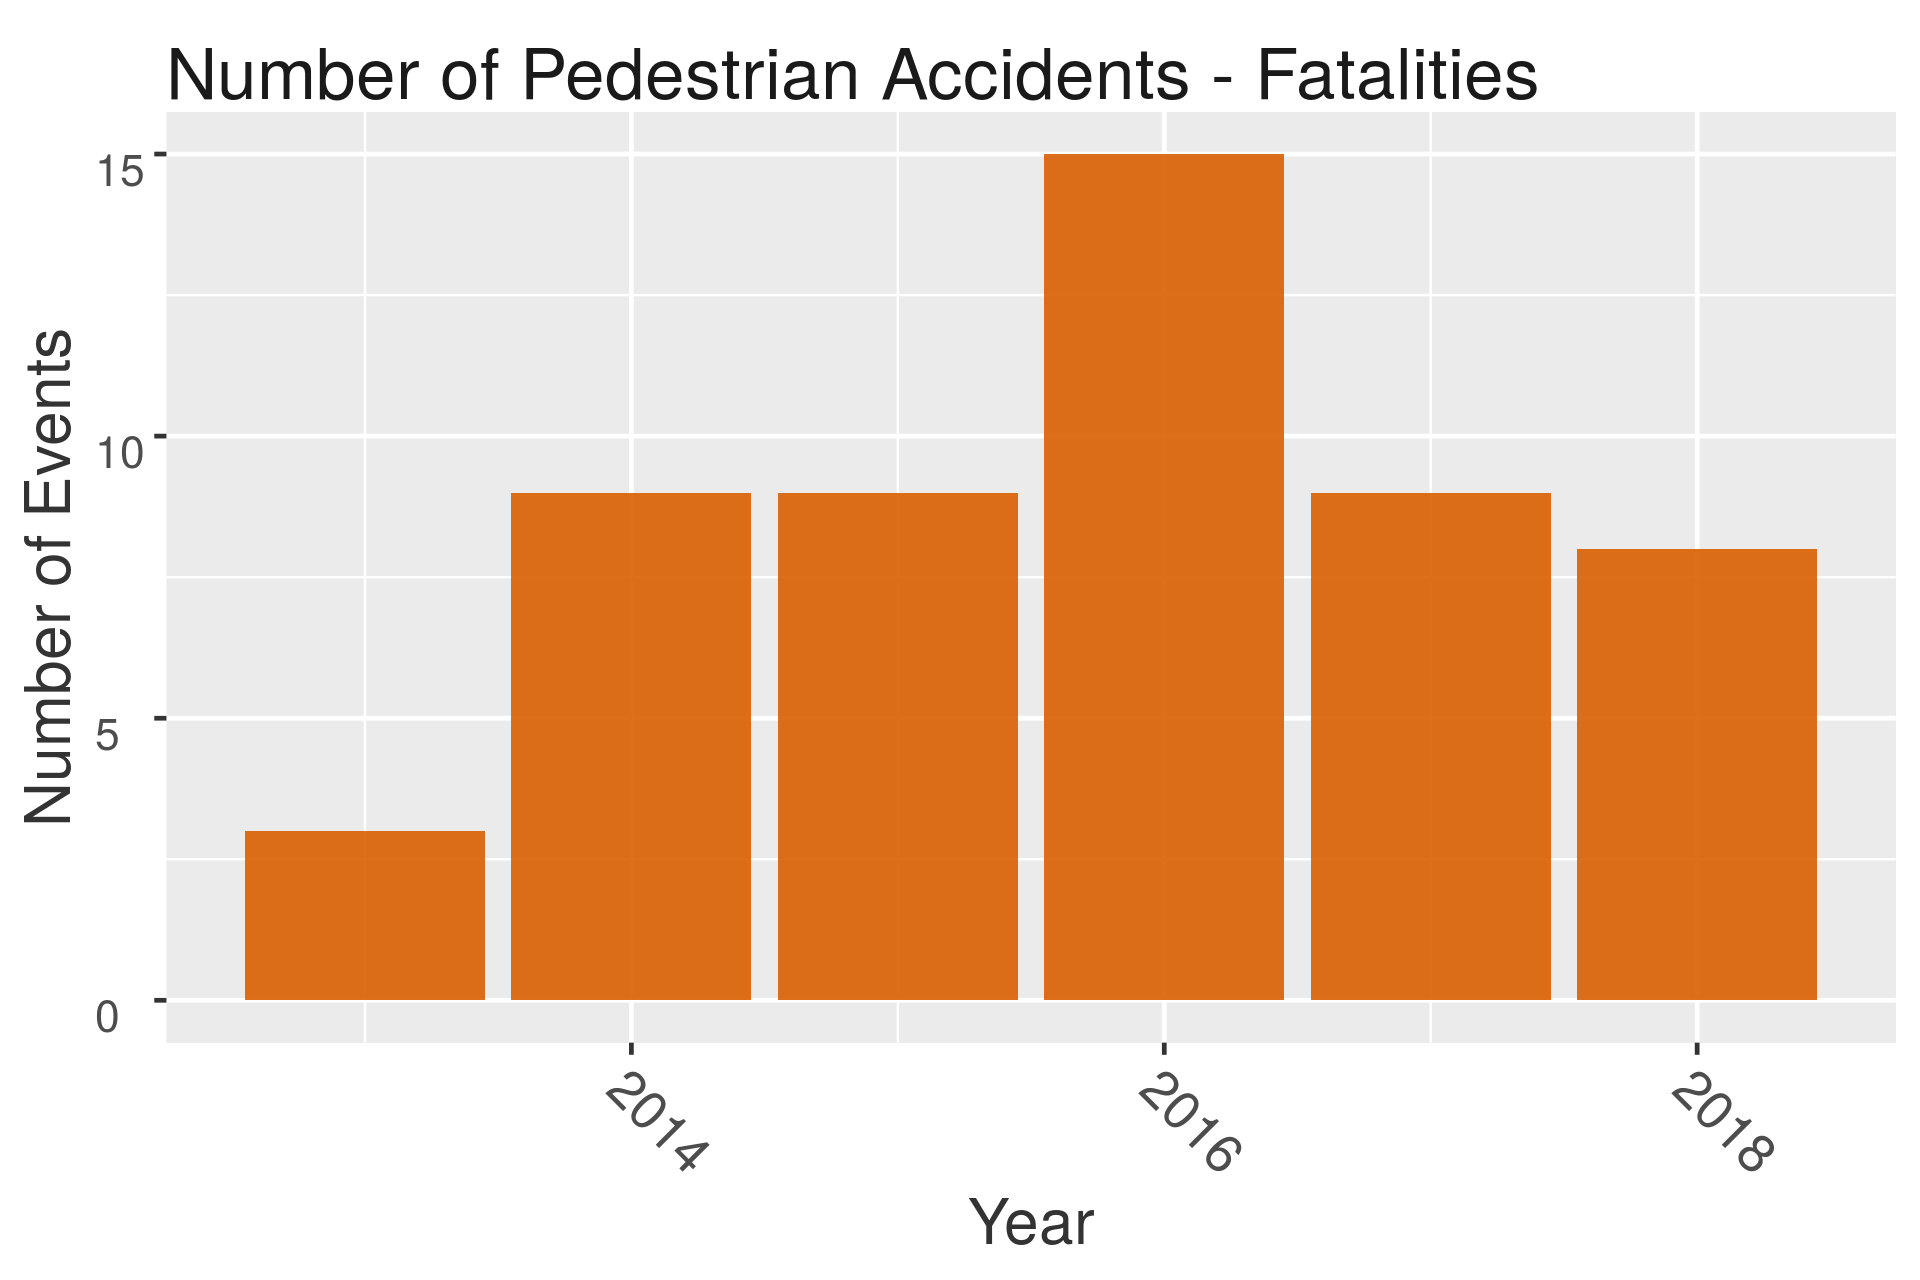
\includegraphics[width = \textwidth, height = \textheight, keepaspectratio]{pedestrianAccidentNumFatalities.png}
    	\subcaption{Fatalities}
    	\label{figure : pedestrianAccidentNumFatalities}
  	\end{subfigure}
  %
  \begin{subfigure}[b]{0.5\textwidth}
    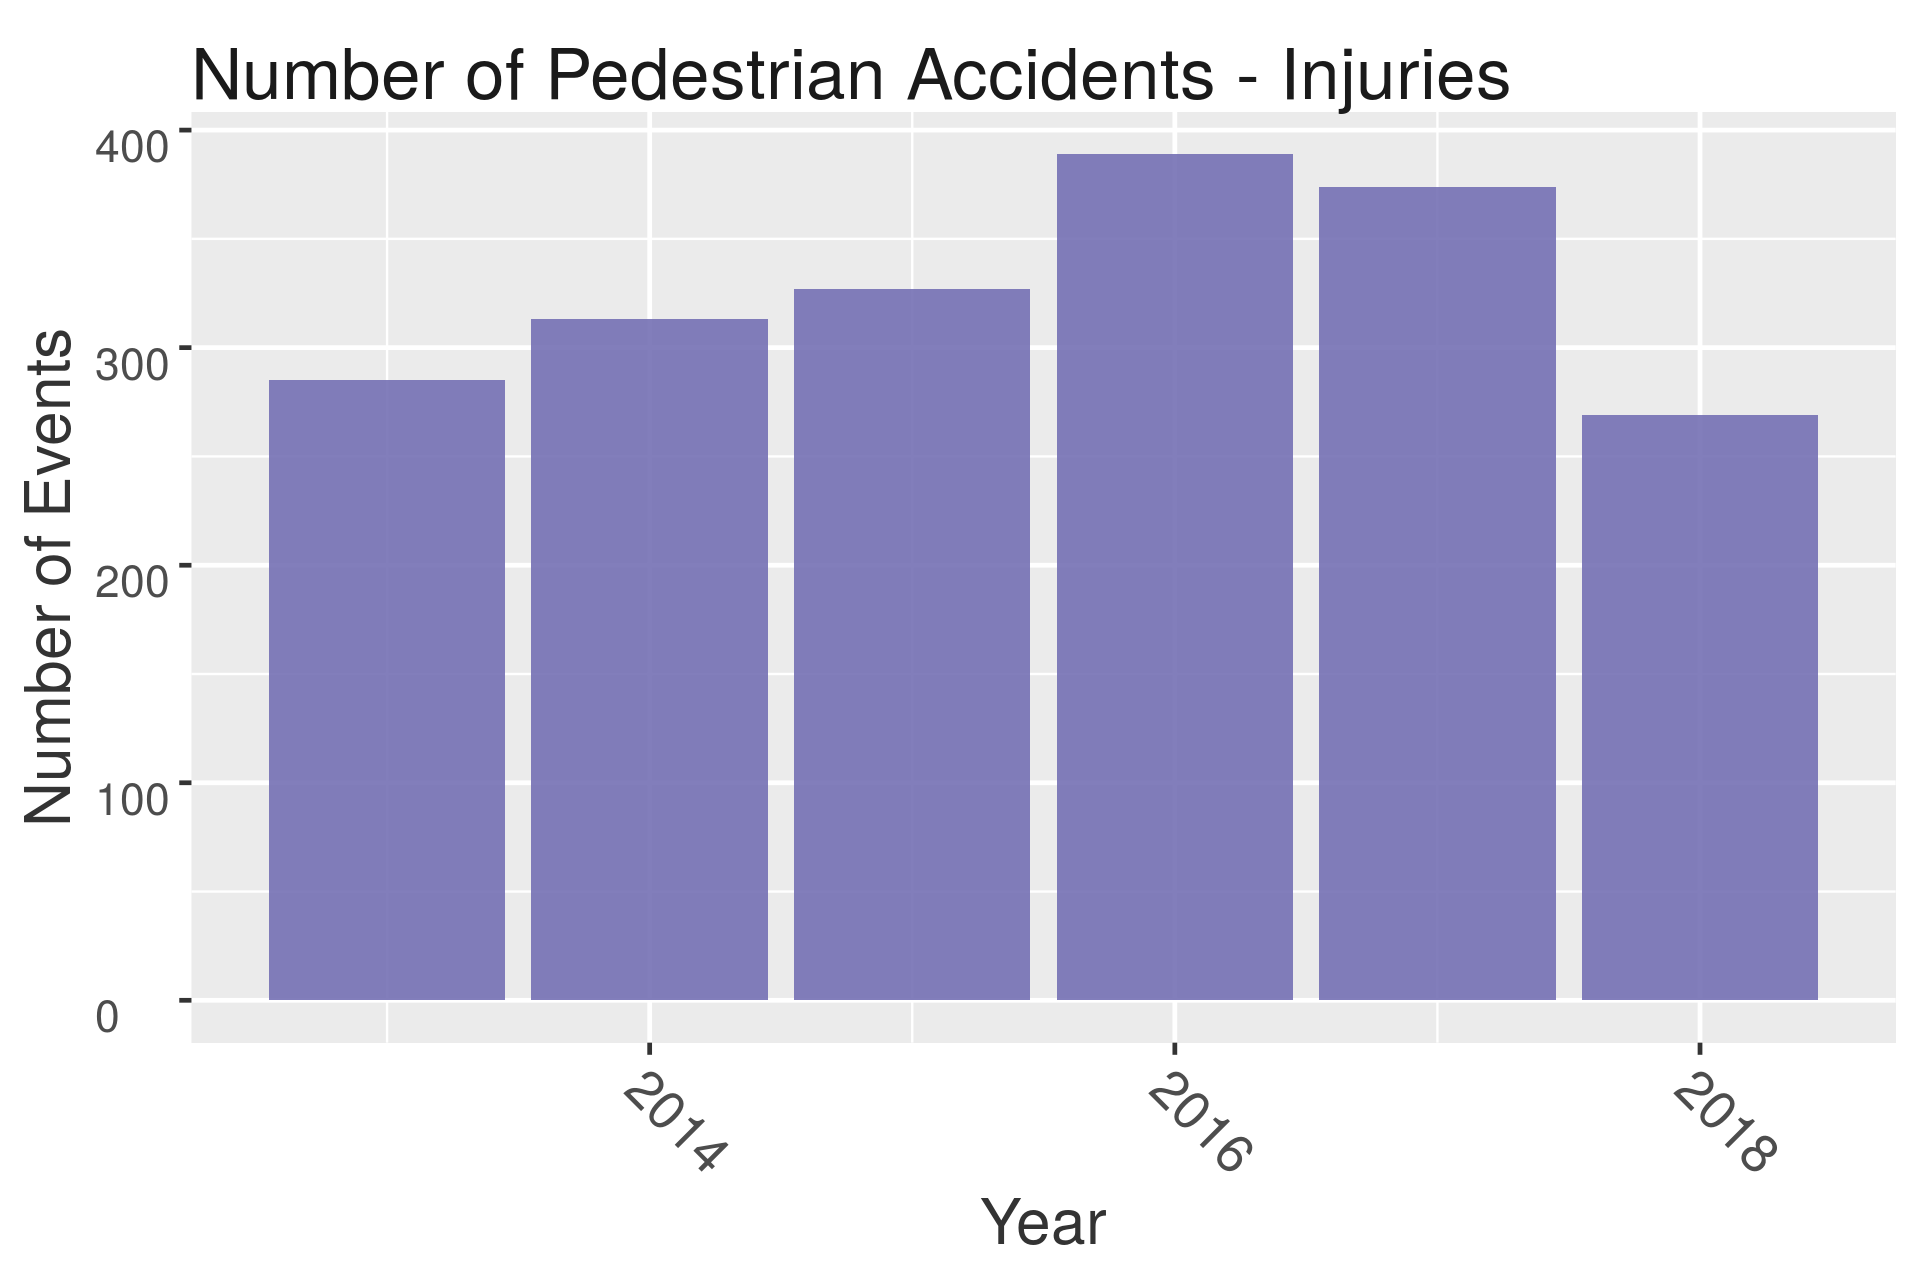
\includegraphics[width = \textwidth, height = \textheight, keepaspectratio]{pedestrianAccidentNumInjuries.png}
    \subcaption{Injuries}
    \label{figure : pedestrianAccidentNumInjuries}
  \end{subfigure}
\end{figure}
\FloatBarrier

\section{Pedestrian Safety}
%
The subject pedestrian safety is supported by terminology specific to this domain. A collection of the terminology that we use in this paper is provided in this section. 

Prime measurements that are used to report pedestrian safety events are fatalities, injuries, and near misses. The statistics in these categories are quoted in number of events and are typically stated on an annualized and per capita basis.

There are a range of severities associated to the outcomes of pedestrian--vehicle accidents. A continuous real valued response variable that accounts for the both the severity and the frequency of events can be established by accounting for this relative severity. We implement a response variable that is a multiple of the number of events and the cost of the event. The cost basis that we use is based on average severity costs for 5 levels of events, as established by the National Safety Council\footnote{https://www.nsc.org/Portals/0/Documents/NSCDocuments_Corporate/estimating-costs.pdf} as shown in Table ~\ref{table:eventseverity}. As identified in the NSC estimating method are not the actual incurred economic costs, but also include estimations for lost quality of life. The values in the Table \ref{eventseverity} are for a per-injured person basis. For our purposes, the actual costs are not used to establish an actual economic impact, but are used to represent a relative severity among the injury types. For instance, a fatality is assessed to be ten times more severe than a disabling injury and two hundred times more negatively impactful than an event where no injury was observed.

%
\FloatBarrier
\begin{table}[!h]
\begin{center}
\caption{Event Comprehensive Cost Severity, National Safety Council}
\label{table:eventseverity}
\begin{tabular}{lr}
%{p{50mm}  p{50mm}}
\hline
\rule{0pt}{12pt}
Severity & Unit Cost (\$)\\[2pt]
\hline
Fatality 			&10,082,000\\
Disabling Injury 		&1,103,000\\
Evident Injury 		&304,000\\
Possible injury 		&141,000\\
No Injury Observed		&46,600\\[2pt]
\hline
\end{tabular}
\end{center}
\end{table}
\FloatBarrier
%
Table ~\ref{table:terminology} provides definitions of  pedestrian safety related terminology as used in this paper.
%
\FloatBarrier
\begin{table}[!ht]
\caption{Pedestrian safety terminology}
\label{table:terminology}
\begin{center}
\begin{tabular}{ p{.50\textwidth}  p{.50\textwidth} }
\hline
\rule{0pt}{12pt}
Attribute & Description\\[2pt]
\hline
Potential for Safety Improvement (PSI)	&	Measures the actual crash cost minus the expected cost of “similar” sites that can be obtained from the crash cost models. In typical usage, an explanatory model using available features is established to predict some measure of cost (e.g., fatality or injury). \cite{ohgov2017} \\		
Hotspot & Areas with higher density or frequency of pedestrian related accidents \cite{xie2017analysis}. 	\\	[2pt]
\hline
\end{tabular}
\end{center}	
\end{table}
\FloatBarrier	

The focus of many pedestrian safety studies is the interaction between pedestrians and vehicles. Prior works have created statistical models to determine the likelihood of crashes, given information about the time of day, victim's age, gender, and other features \cite{brude1993models} \cite{lascala2000demographic} \cite{lyon2002pedestrian} \cite{ladron2004forecasting} \cite{pulugurtha2011pedestrian} \cite{ukkusuri2011random}. The study done by Guo \cite{guo2017effect}, et al examined the patterning and structure of road networks as a factor of pedestrian vehicle interactions (PVIs). Zhang et al \cite{zhang2017quantitative} created a statistical model that classified different types of street crossings to determine which type of crossing was the safest, and gain insight to the relationships between the factors that contribute to a PVI. 


In our study, we address the issue of pedestrian safety in a manner that is generally consistent with traffic safety analysis methods, which develop a model, typically via linear regression,  and then use the variance between expected and observed to determine the areas with potential for improvement as the areas in which the observed number (or cost severity) of events most greatly exceeds the model expected values. Common in highway traffic studies is the implementation of an empirical Bayesian adjustment to the regression model estimations.

\begin{equation} Expected_{Bayesian} = \eta \cdot P(E)  + (1 - \eta) \cdot O(E),
\end{equation} \newline
where $0 < \eta < 1$, $P(E)$ = expected accidents (either in severity or number) from the model for similar locations, and
$O(E)$ is the observed accidents (either in severity or number) for a specific location. $\eta$ is determined empirically from existing models or published standards from, for example, the National Highway Transportation Association. (NEED REFERENCE HERE)

We do not implement that additional step, as our purpose is restricted to identifying locations that have greatest positive variance (observed - expected) in comparison to all of the other grid cells in the modeled region. For this purpose, it is not additional added value to include the adjustment associated to the empirical Bayesian procedure.

<Place holder for supervized learning solution>
The unsupervized learning we have generated clusters of pedestrian safety issues and visualized them on the grid map of Cincinnati
<Place holder for supervized learning results>
unsupervized learning results
<Place holder for supervized learning conclusion>
unsupervized learning conclusion

The remainder of this paper is organized as follows. In Section 2 we provide general information about pedestrian safety, terminology used in subsequent sections of the study, and a valuation associated to the costs incurred in pedestrian accidents. In Section 3 we describe the data sources and data sets used in this study, a description of a grid cell approach to modeling geographic data, the development of model features from the source data, and some graphical representations of the distribution of these features viewed geographically. In section 4 we describe the various models implemented, the results and analysis of the results are presented in Sections 5 and 6. Ethical considerations of this study are provided in Section 7. The Conclusion is presented in Section 8. 

% ...		-=-=-=-=-=-=-=-=-=-=-=-=-=-=-=-=-=-=-=-=-=-=-=-=-=-=-=-=-=-=-=-=-=-=-=-=-=-
\section{Data Sets}
% ...		-=-=-=-=-=-=-=-=-=-=-=-=-=-=-=-=-=-=-=-=-=-=-=-=-=-=-=-=-=-=-=-=-=-=-=-=-=-


\subsection{Grid cell development}

To enable the development of both supervised and unsupervised learning models, we employ a grid cell approach. We superpose a grid of equi-distant points over the geographic definition of the city of Cincinnati. The grid points are spaced at approx 250 meter distance. This provides a uniform distribution of 4,196 grid cells to encompass the 80 square mile surface area of the city. Our approach then is to assemble all of the experiences from the various data sources that occurred within a grid cell as representative of that area's experience. The supervised learning model then consists of 4,196 rows (representing each individual grid cell in the map) and as many columns as data features that we complete as independent estimators of the dependent response. In the following descriptions of data sets, we display them in the aggregated grid cell to visualize the relative density of each feature within the city boundaries. 

The development of the grid cells, the feature definition from each data set, and the aggregation of the response variables and independent features are all completed using customized R code.

Our rationale for using 250m grid spacing was chosen as a baseline distance for model development. It represents a distance that is intermediate in comparison to other studies using similar approaches\cite{xie2017analysis}. This is a characteristic of the modeling approach that can be considered for optimization in future evaluations or developed as a hyper-parameter to improve model performance.

% ...		---------------------------------------------------------------------------------------------------------

\subsection{Open Data Cincinnati}

Like many cities in the US, Cincinnati is also a participant in the Open Data experiment. The city makes accessible the government data freely available to the public with the goal that interested individuals and groups will use the data sets in creative ways to improve the quality of life in the city. The source of much of the data that we utilize in this study is accessed from the Cincinnati Open Data portal. Our method was to review each data set accessible from the web portal, intuit whether that data set potentially provided relevant information to include in a predictive model related to pedestrian safety, and if so, download that data set to a local hard drive for future processing. The basis for retaining a data set for incorporation in the model was based on the assumption that data sets that provide information for a five year period, with quantifiable characteristics that characterize infrastructure related to transportation (street density and locations, public transportation accessibility), services provided by the city (non-emergency service calls), and information directly related to traffic and pedestrian accidents. From this basic approach, we identified the data sets as shown in Table \ref{table : cincinnatidatasets}

In addition to the data available on the Open Data Cincinnati portal, we also utilize two data sets obtained directly from the city's Department of Transportation \& Safety (DOTE). The first of these is the result of a survey that was conducted from February through April 2018. The second is reports of near-miss interactions between pedestrians and vehicles that were independently reported to the city DOTE and retained in a separate database. Both of these data sets were provided to us for our use in this evaluation. Both of these data sets are further explained in a subsequent section of this paper.

Augmenting the data sets available from the City of Cincinnati, we also use data available from two additional sources. Walk Score\textsuperscript{\tiny\textregistered}\footnote{https://www.walkscore.com/}

\FloatBarrier
\begin{table}[!h]
\begin{center}
\caption{Cincinnati based data sets}
\label{table:cincinnatidatasets}
\begin{tabular}{ p{.25\textwidth}  p{.30\textwidth}  p{.45\textwidth}}
\hline
\rule{0pt}{12pt}
Data Set
	& Source
	& Evaluation summary\\[2pt]
\hline
Cincinnati open data
	& https://data.cincinnati-oh.gov
	& Contains economic, neighborhood safety, and health related data for city of Cincinnati\newline
	Data is not granular\\
Cincinnati pedestrian safety survey data
	&
	& 
	Contains survey data from citizens who have reported problems by using the web-page\newline
	Data is organized at  the street intersection level\newline
	  Data was collected from Feb - Apr 2018\\
Pedestrian near miss data
	&
	& A dataset provided by the city of Cincinnati containing latitude and longitudinal data of near-miss incidents within the city\\
Income and house price
	& http://www.city-data.com/nbmaps/neigh-Cincinnati-Ohio.html
	& Contains statistics on age, house prices, income and more\newline
	Data gathered as a collection of public and private sources\newline
	Data organized at both the neighborhood, and census block group level\\[2pt]
\hline
\end{tabular}
\end{center}
\end{table}
\FloatBarrier
%
\FloatBarrier
\begin{table}[!ht]
\caption{Cincinnati open data datasets}
\label{table:cincinnatiopendata}
\begin{center}
\begin{tabular}{p{40mm}  p{80mm}}
\hline
\rule{0pt}{12pt}
Data Set & Evaluation Summary\\[2pt]
\hline
Cincinnati 311 non-emergency service requests 
	& This dataset contains records of all non-emergency service requests to the city of Cincinnati from 2012 to 2018. Contains reports from graffiti to relevant traffic information such as 		roadkill and potholes.\\	
2017 NFIRS Cincinnati Fire Department Incident Data 
	& National Fire Incident Reporting System dataset which reports on the full range of fire deparment activities with reports of number of employees and vehicles deployed to every 			incident.\\	
Street Centerline (w/ PCI rating) 
	& City street centerline data with pavement condition index ranking; used to determine road condition and composition.\\	
Traffic Crash Reports (CPD)
	 & The Cincinnati traffic crash reports dataset compiled by the Cincinnati Police Department. It contains records of responses to traffic crashes, containing a wide-range of crash data 		such as persons involved, injury level, day, time, and weather.\\	[2pt]
\hline
\end{tabular}
\end{center}	
\end{table}

%

\begin{table}[!h]
\begin{center}
\caption{Supplementary data sets}
\label{table:supplementarydatasets}
\begin{tabular}{ p{.20\textwidth}  p{.35\textwidth}  p{.45\textwidth}}
\hline
\rule{0pt}{12pt}
Data Set
	& Source
	& Evaluation summary\\[2pt]
\hline
Google Maps
	& https://developers.google.--\newline
		com/maps 
	& This API gives us granular data on walking and biking - distance, direction and other information\newline
	Latitude and Longitude information for grid areas can be derived using this API\\
Walk Score\textsuperscript{\tiny\textregistered}
	&https://www.walkscore	\newline
	.com
	&A scoring scale across US which gives an idea of the current walkability of the city\\
Zillow
	& https://www.quandl.com/ \newline
	data/ZILLOW/M26_NFS-Zillow \newline
	-Home-Value-Index-Metro-NF- \newline
	Sales-Cincinnati-OH
	& The Zillow Home Value Index contains monthly time-series of data which represent Zillow's estimation of the median market value of home sales.\\[2pt]
\hline
\end{tabular}
\end{center}
\end{table}
\FloatBarrier
%

% ...		---------------------------------------------------------------------------------------------------------

\subsubsection{Pedestrian Accidents}

From the Open Data Cincinnati portal, we use the data set Traffic Crash Reports (CPD) to identify the pedestrian accident history. From this data set, there are more than 2,100 reported events involving pedestrians in the years 2013 through 2018. Of these, there are 47 reported fatalities, 2008 injuries, and 109 events reported as property damage only. The annual count for fatalities and injuries are shown in Table \ref{figure : pedestrianAccidentsAnnual}. As a dependent response characteristic for this model, we distribute each of the events to the appropriate grid cell, apply the comprehensive cost severity factor as identified in Table \ref{table : eventseverity}, aggregate the total experience in each grid cell as a dollar severity amount, and then apply a kernel function to distribute the cost severity over the local geographic region. The kernel function approach is employed with the premise that local conditions, beyond just the perimeter of a 250m x 250m region in which the accident occurred, participate in providing the conditions that contribute to a pedestrian accident. Further, the kernel function acts to develop a more continuous distribution of event costs which would otherwise be localized discontinuous point functions with grid cells of high severity being surrounded by grid cells with zero cost. For our purposes, we use a kernel function radius of 0.005 degrees (latitude or longitude). This provides a radius search distance of adjacent grid cells of approximately 500 meters, resulting in the cost severity being distributed to approximately 15 neighboring grid cells.  Similar to the decision to use 250m grid spacing for the model, we use the 500m radius inclusion distance for this model as it represents a distance that is intermediate in comparison to other studies using similar approaches. This is a characteristic of the modeling approach that can also be considered for optimization in future evaluations or developed as a hyper-parameter to improve model performance.

The kernel density function that we use distributes the cost severity spatially using the following quartic function\cite{xie2017analysis} : 
\begin{align}
Cost_{g} = \sum_{i=1}^{n} \rho_{i} \left [ 1 - \left ( \frac{d_{ig}}{r} \right )^{2} \right ]^{2}C_{i},
\end{align}

where $Cost_{g}$ is the crash cost assigned to grid cell $g$, $d_{ig}$    is the distance from the identified pedestrian accident site to the local grid cell centroids, $r$ is the (constant) search radius, $C_{i}$ is the cost severity of the accident ${i}$, and $\rho_{i}$ is a normalizing factor for each accident such that the distributed costs for each accident sum to the nominal severity value of that event. For our model, the implementation of this kernel density function was implemented within the R code.

The distribution that results from the application of this data set onto the grid cell domain with the kernel density function applied are shown in figure \ref{figure : PedestrianCosts}. The experience is that approximately $\frac{1}{4}$th of the grid cells have no contribution from the cost severity allocation and the remaining $\frac{3}{4}$ths demonstrate a reasonable approximation to a log-normal distribution of allocated costs. For clarity in the figures, the cost values in Figure  \ref{figure : pedestrianAccidentCostsHistogram} are shown log-transformed [log10(cost)], and the zero values scaled as log10(0.1).


% ... pedestrian accident distributions

\FloatBarrier
\begin{figure}
 	\caption{Pedestrian Accidents - Comprehensive Cost Severity (\$ Millions)}
    \label{figure : PedestrianCosts}
  \begin{subfigure}[b]{0.5\textwidth}
    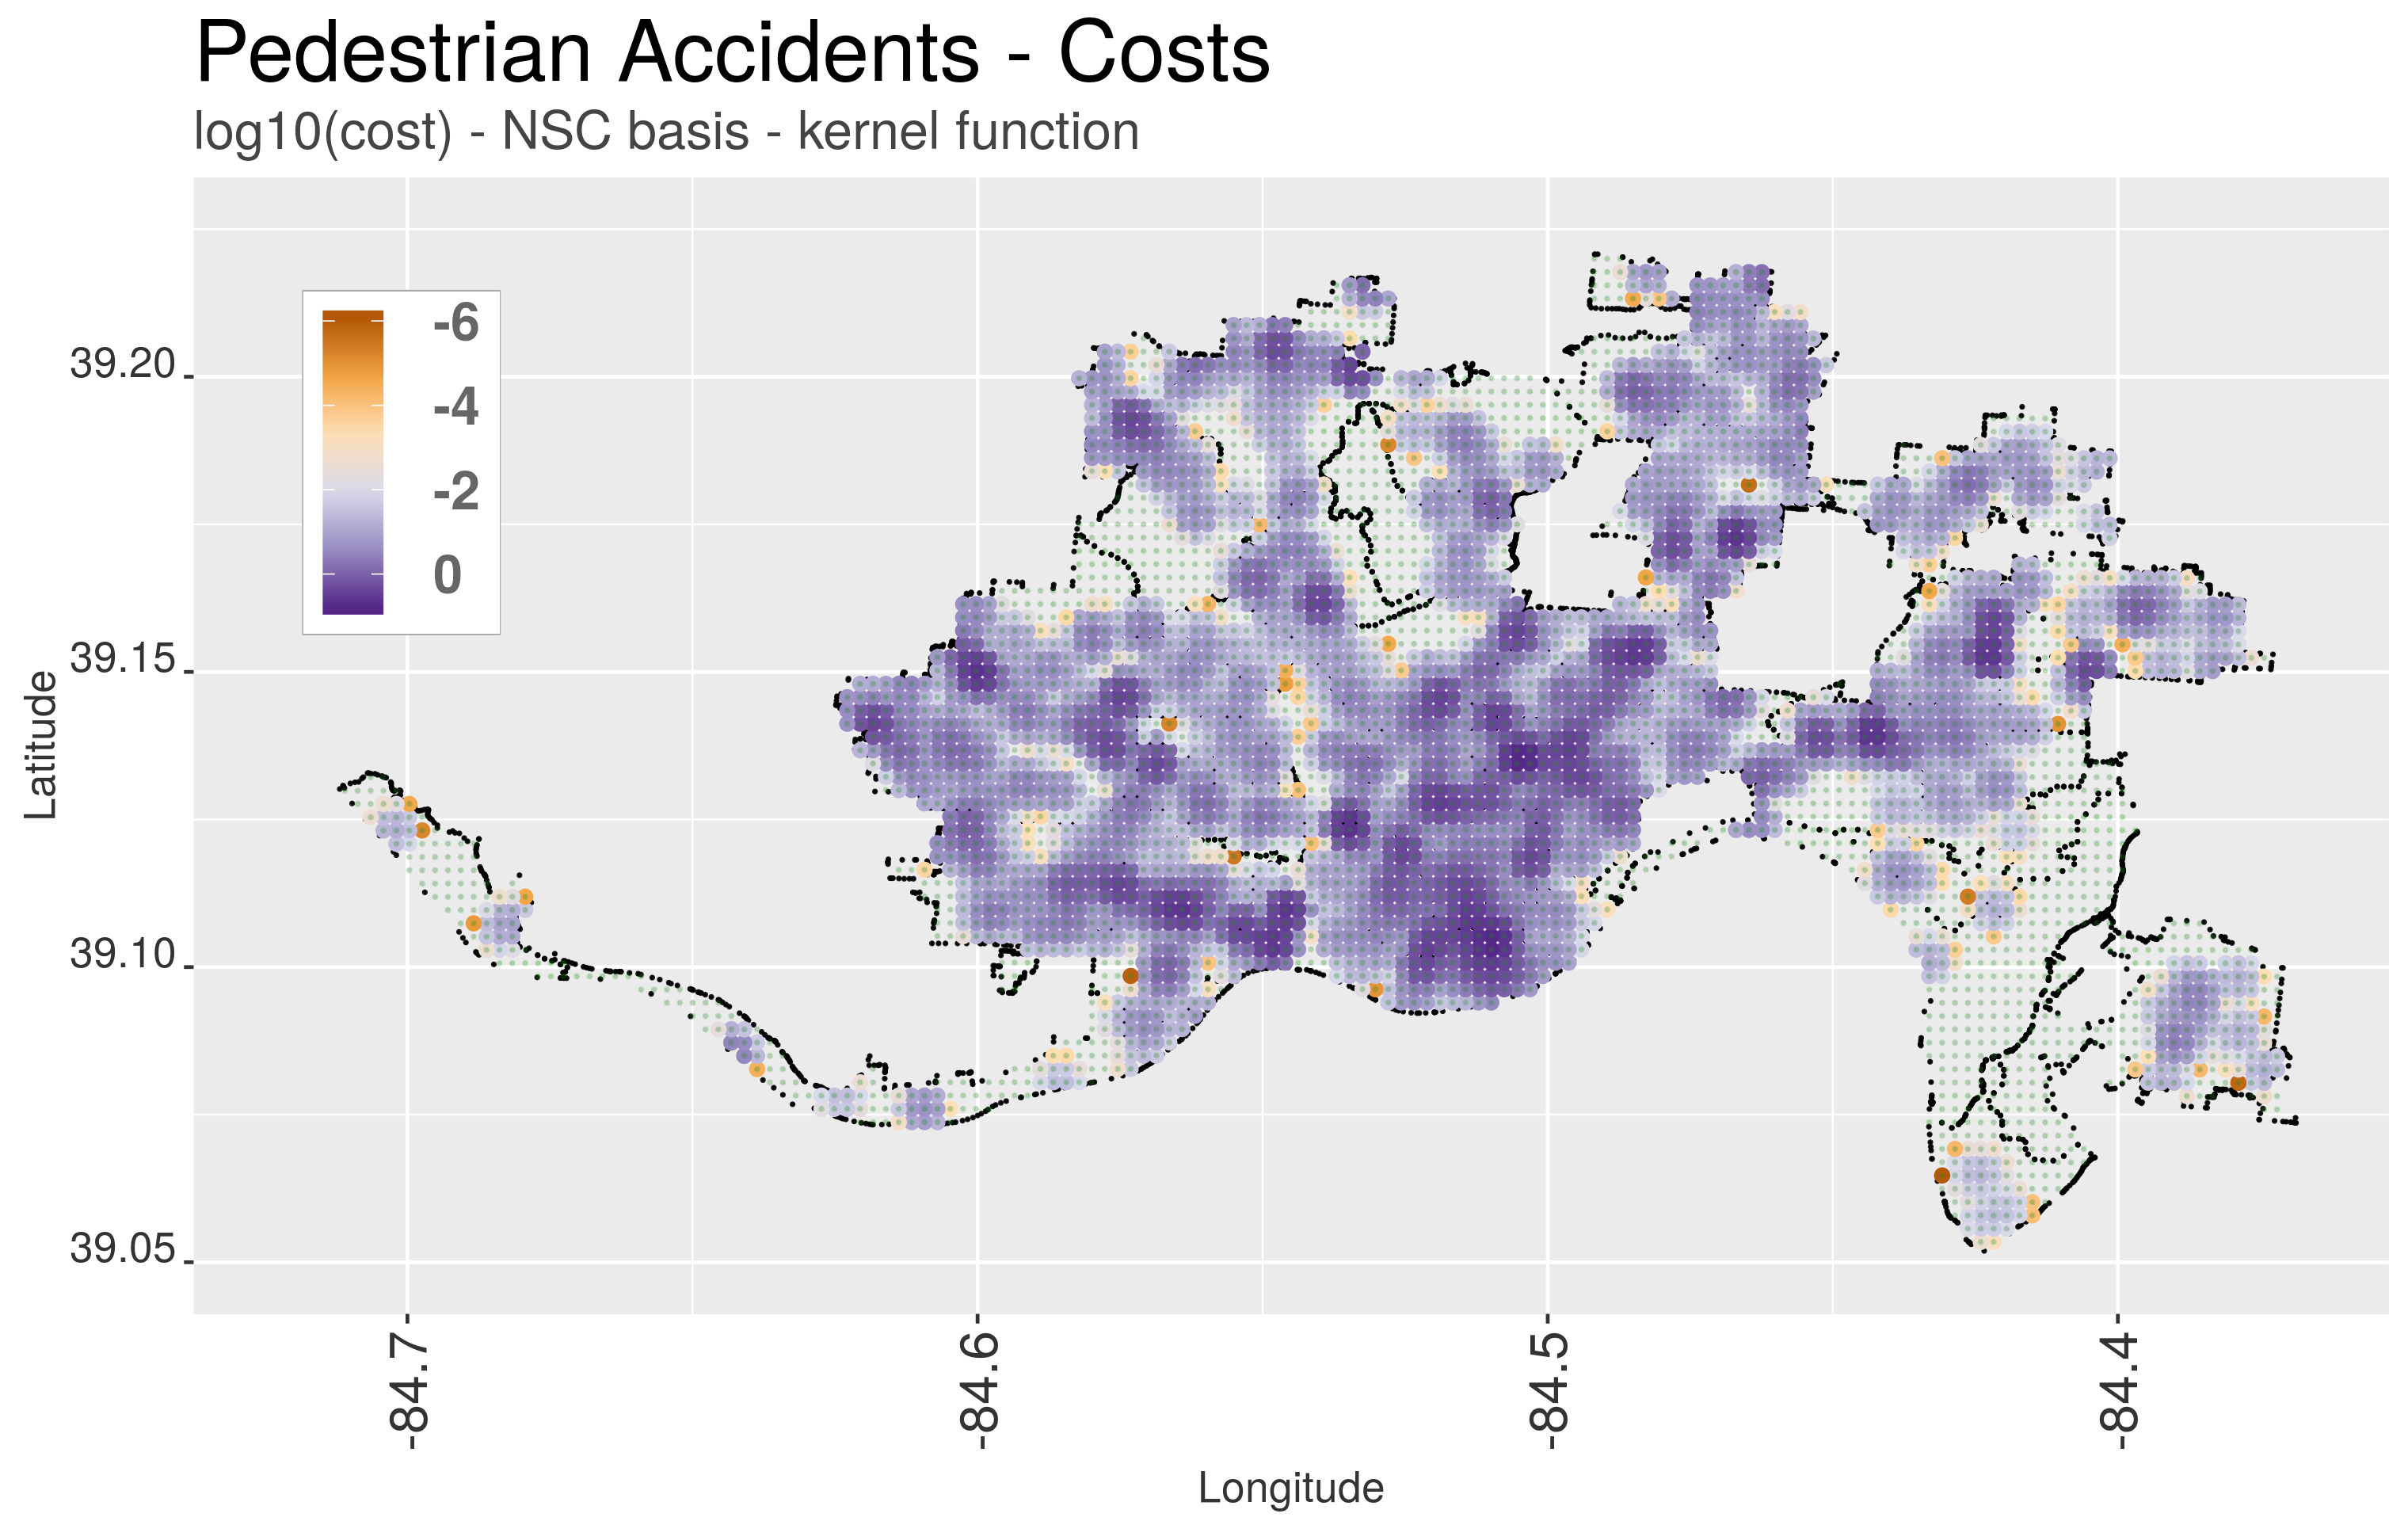
\includegraphics[width = \textwidth, height = \textheight, keepaspectratio]{trafficAccidentsPedestrianCosts.png}
    \subcaption{Geographic Distribution}
    \label{figure : trafficAccidentsPedestrianCosts}
  \end{subfigure}
  %
  \begin{subfigure}[b]{0.5\textwidth}
    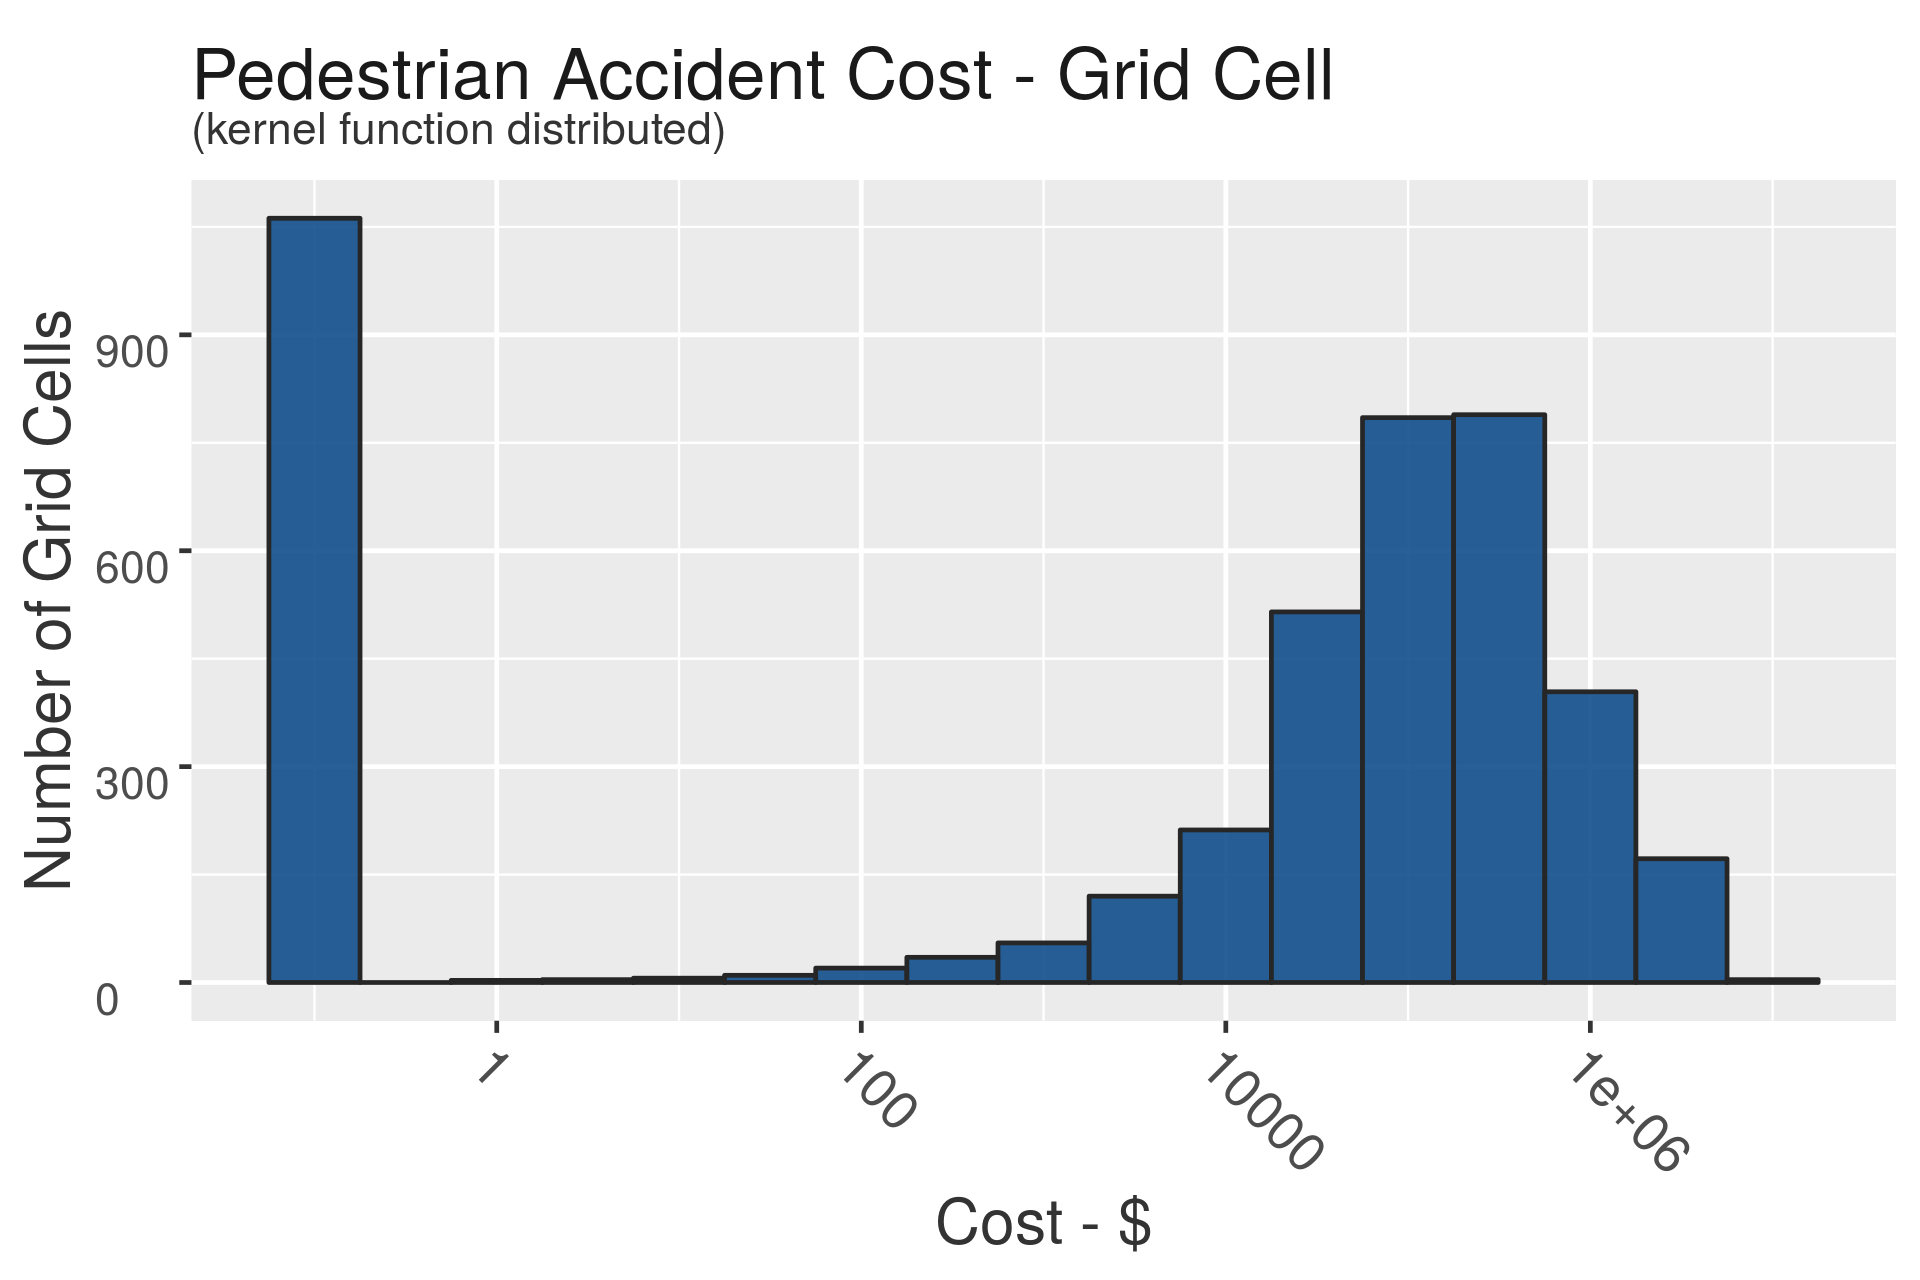
\includegraphics[width = \textwidth, height = \textheight, keepaspectratio]{pedestrianAccidentCostsHistogram.png}
    \subcaption{Distribution}
    \label{figure : pedestrianAccidentCostsHistogram}
  \end{subfigure}
\end{figure}
\FloatBarrier

This motivates us to consider the supervised learning model as a two-part model : (a) binary estimator to model the presence / absence of pedestrian accident costs, and (b) for the positive case of (a), an estimator of the magnitude of the cost severity function. This will be further outlined in the Methods and Results sections of this paper.

% ...		---------------------------------------------------------------------------------------------------------

\subsubsection{Traffic Accidents}

Similar to the pedestrian accident data set in the previous section, the same data set from the the Open Data Cincinnati portal, Traffic Crash Reports (CPD), also includes a definition of every non-pedestrian involved traffic accident that occurred in the same time period.  There are more than 190,000 reported traffic accidents that do not involve pedestrians in the years 2013 through 2018. As a candidate independent feature characteristic for this model, we distribute each of the events to the appropriate grid cell, apply the same comprehensive cost severity factor as identified in Table \ref{table : eventseverity}, aggregate the total experience in each grid cell as a dollar severity amount. We do not apply a kernel function to distribute the cost severity over the local geographic region for the independent predictor featues. In this case, the density of the actual experience is sufficiently distributed that a kernel function for density diffusion is not needed to achieve wide distribution and sufficient coverage of the accident experience among all of the grid cells. The distribution of the cost severity function for the non-pedestrian involved accidents are shown in Figure \ref{figure : trafficAccidentsNonPedestrian}
% ... bus stop distances

\FloatBarrier
\begin{figure}
 	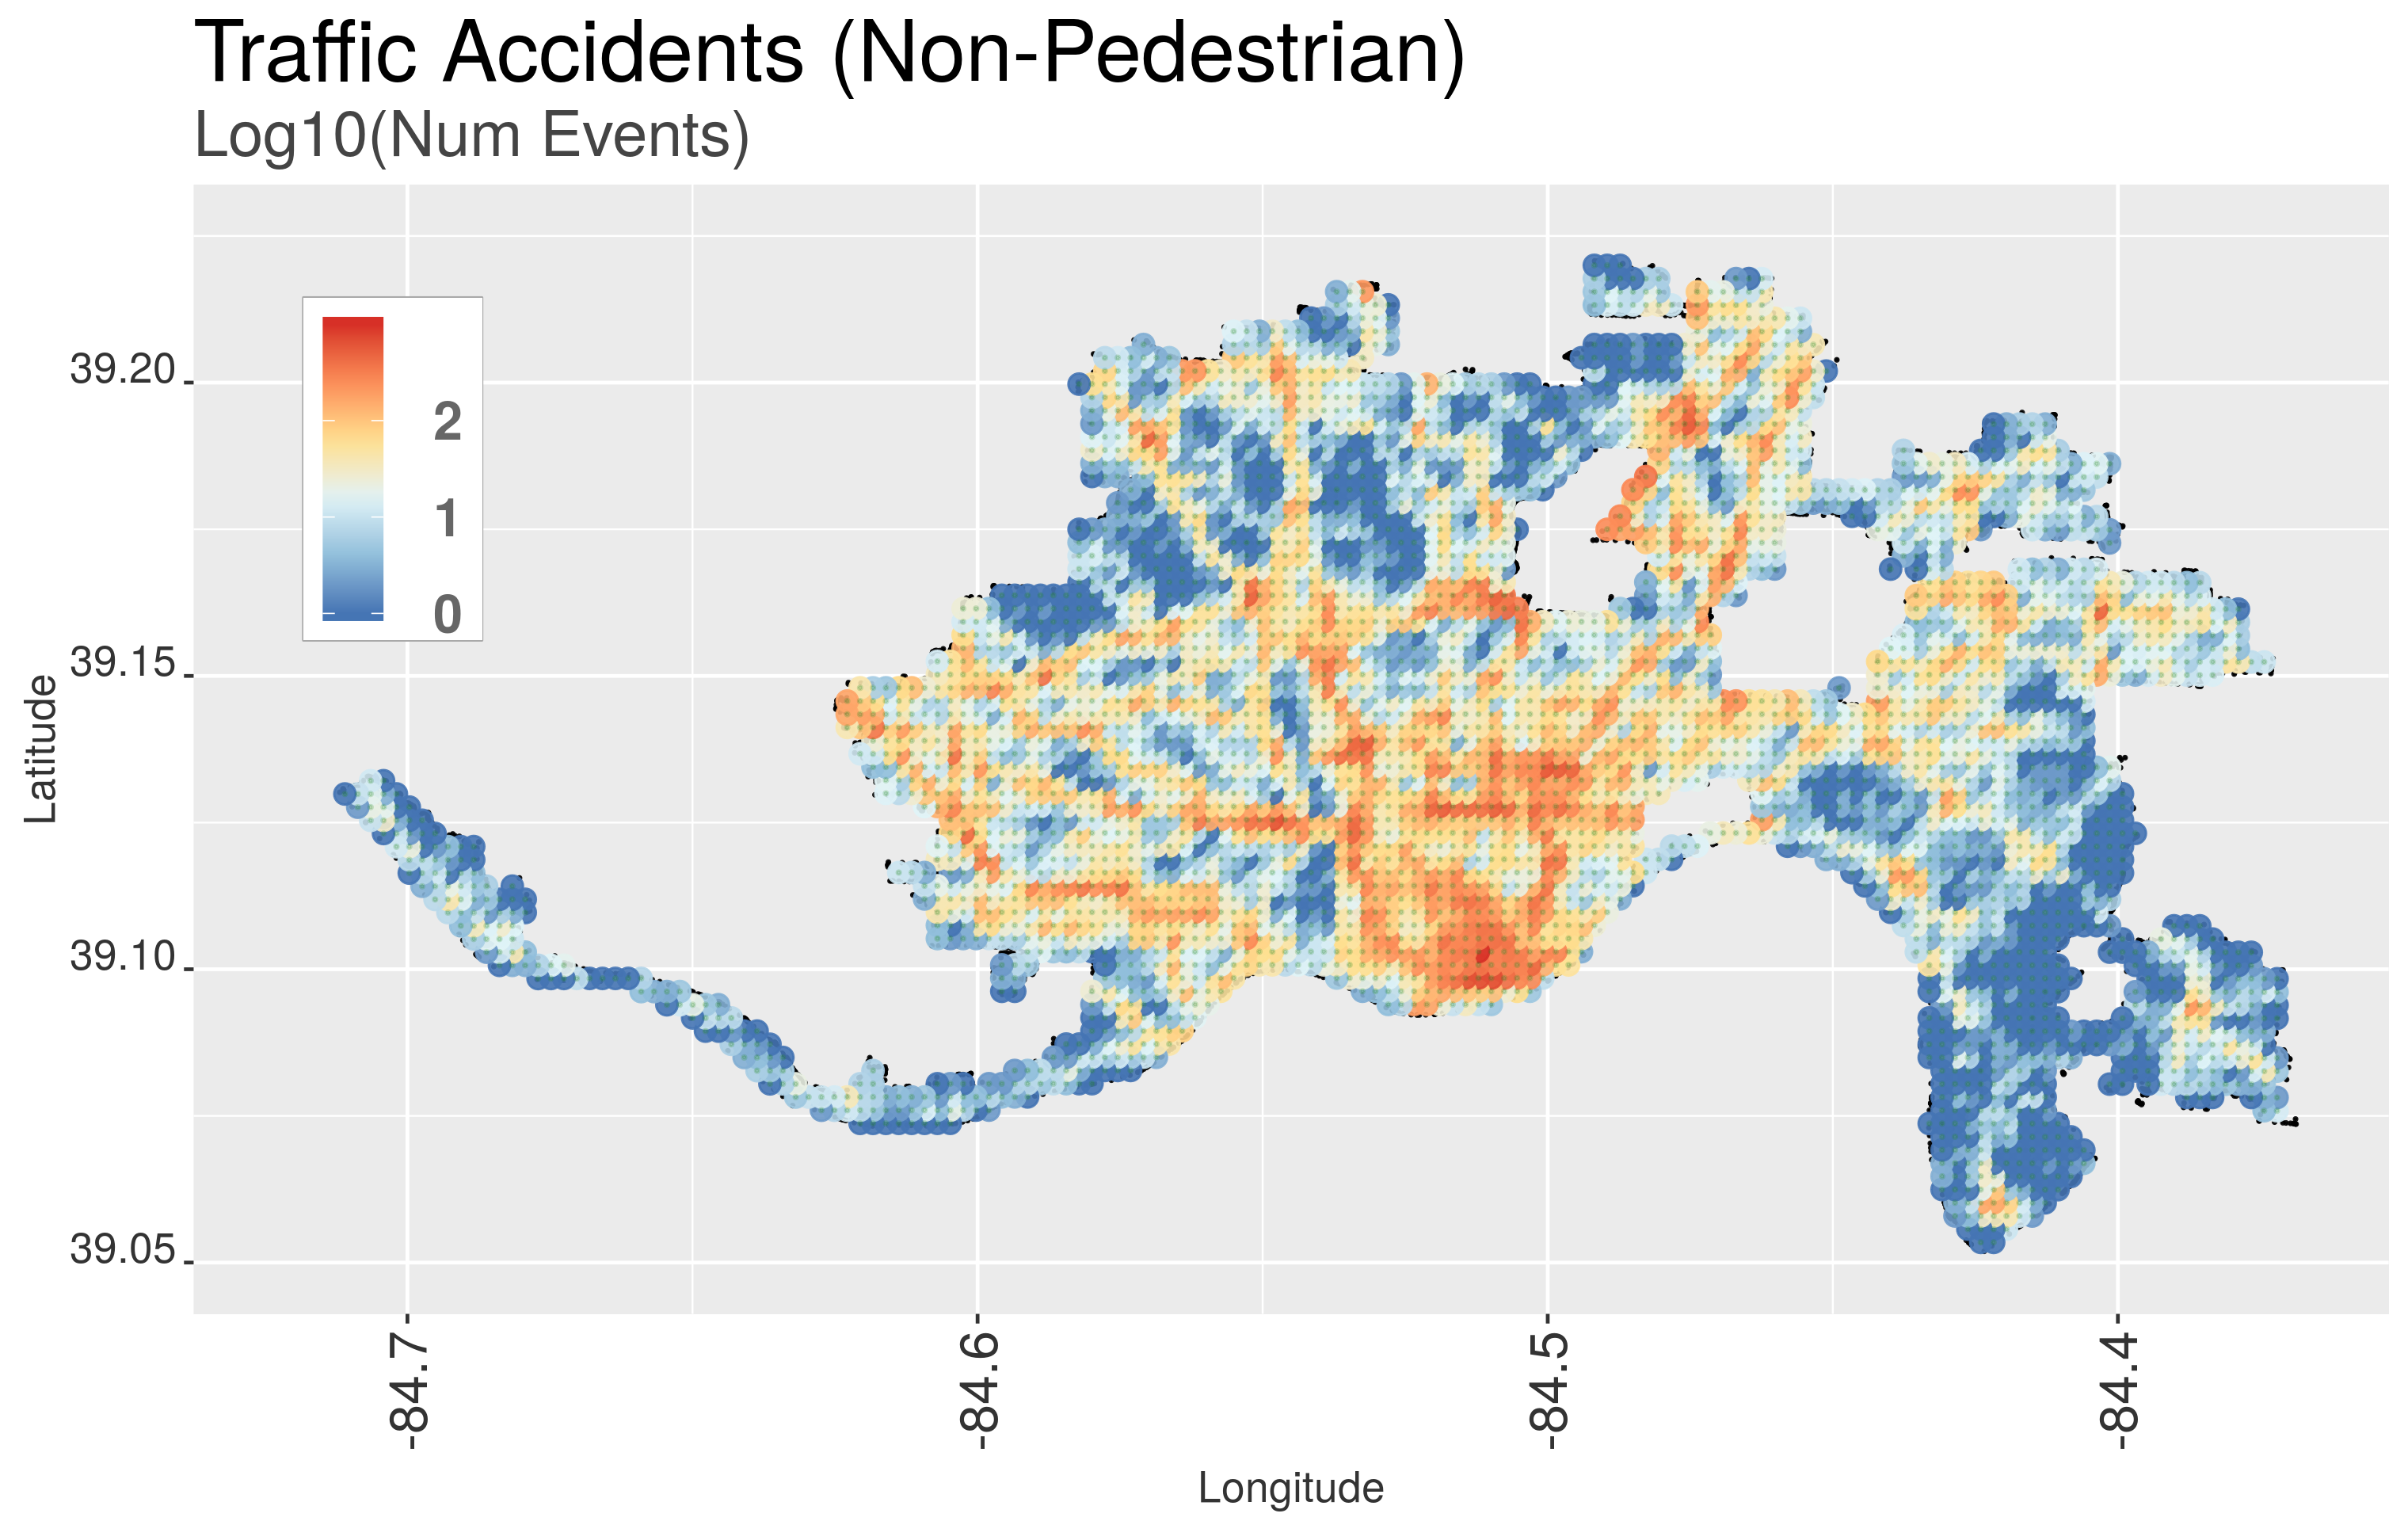
\includegraphics[width=\textwidth, height=\textheight, keepaspectratio]{trafficAccidentsNonPedestrian}
 	\caption{Traffic Accidents - Non-Pedestrian}
	\label{figure : trafficAccidentsNonPedestrian}
\end{figure}
\FloatBarrier

% ...		---------------------------------------------------------------------------------------------------------

\subsubsection{Streets Infrastructure}

Typical traffic safety models include data features to characterize the density of local traffic conditions. For this model in The Open Data Cincinnati portal provides a data set Street Centerlines (w/ PCI rating). This data set includes a description of each street segment in the city and includes the characteristics : geo-locations of the street segment, surface area, surface length, surface width, number of traffic lanes, and the surface type (asphalt, concrete, etc.). We use this data set to develop a set of features as shown in Table \ref{table : streetFeatures}. The statistics shown are summary statistics for the sample of data across all of the grid cells.

\FloatBarrier
\begin{table}[!h]
\begin{center}
\caption{Street surface features}
\label{table : streetFeatures}
\begin{tabular}{lrrr}
%{ p{.9\textwidth}}
\hline
\rule{0pt}{12pt}
Charactertistic	&	1st Quartile	&	Median	&	3rd Quartile	\\[2pt]
\hline
Lane Counts	&	24	&	53	&	108	\\
Sum Widths	&	250	&	563	&	1152	\\
Sum Areas	&	131805	&	284640	&	787812	\\
Number Streets	&	8	&	19	&	38	\\[2pt]
\hline
\end{tabular}
\end{center}
\end{table}
\FloatBarrier
%


The distribution of the sum of street surface area distributed among the grid cells of this model are shown in Figure \ref{figure : streetsSumArea}

\FloatBarrier
\begin{figure}
 	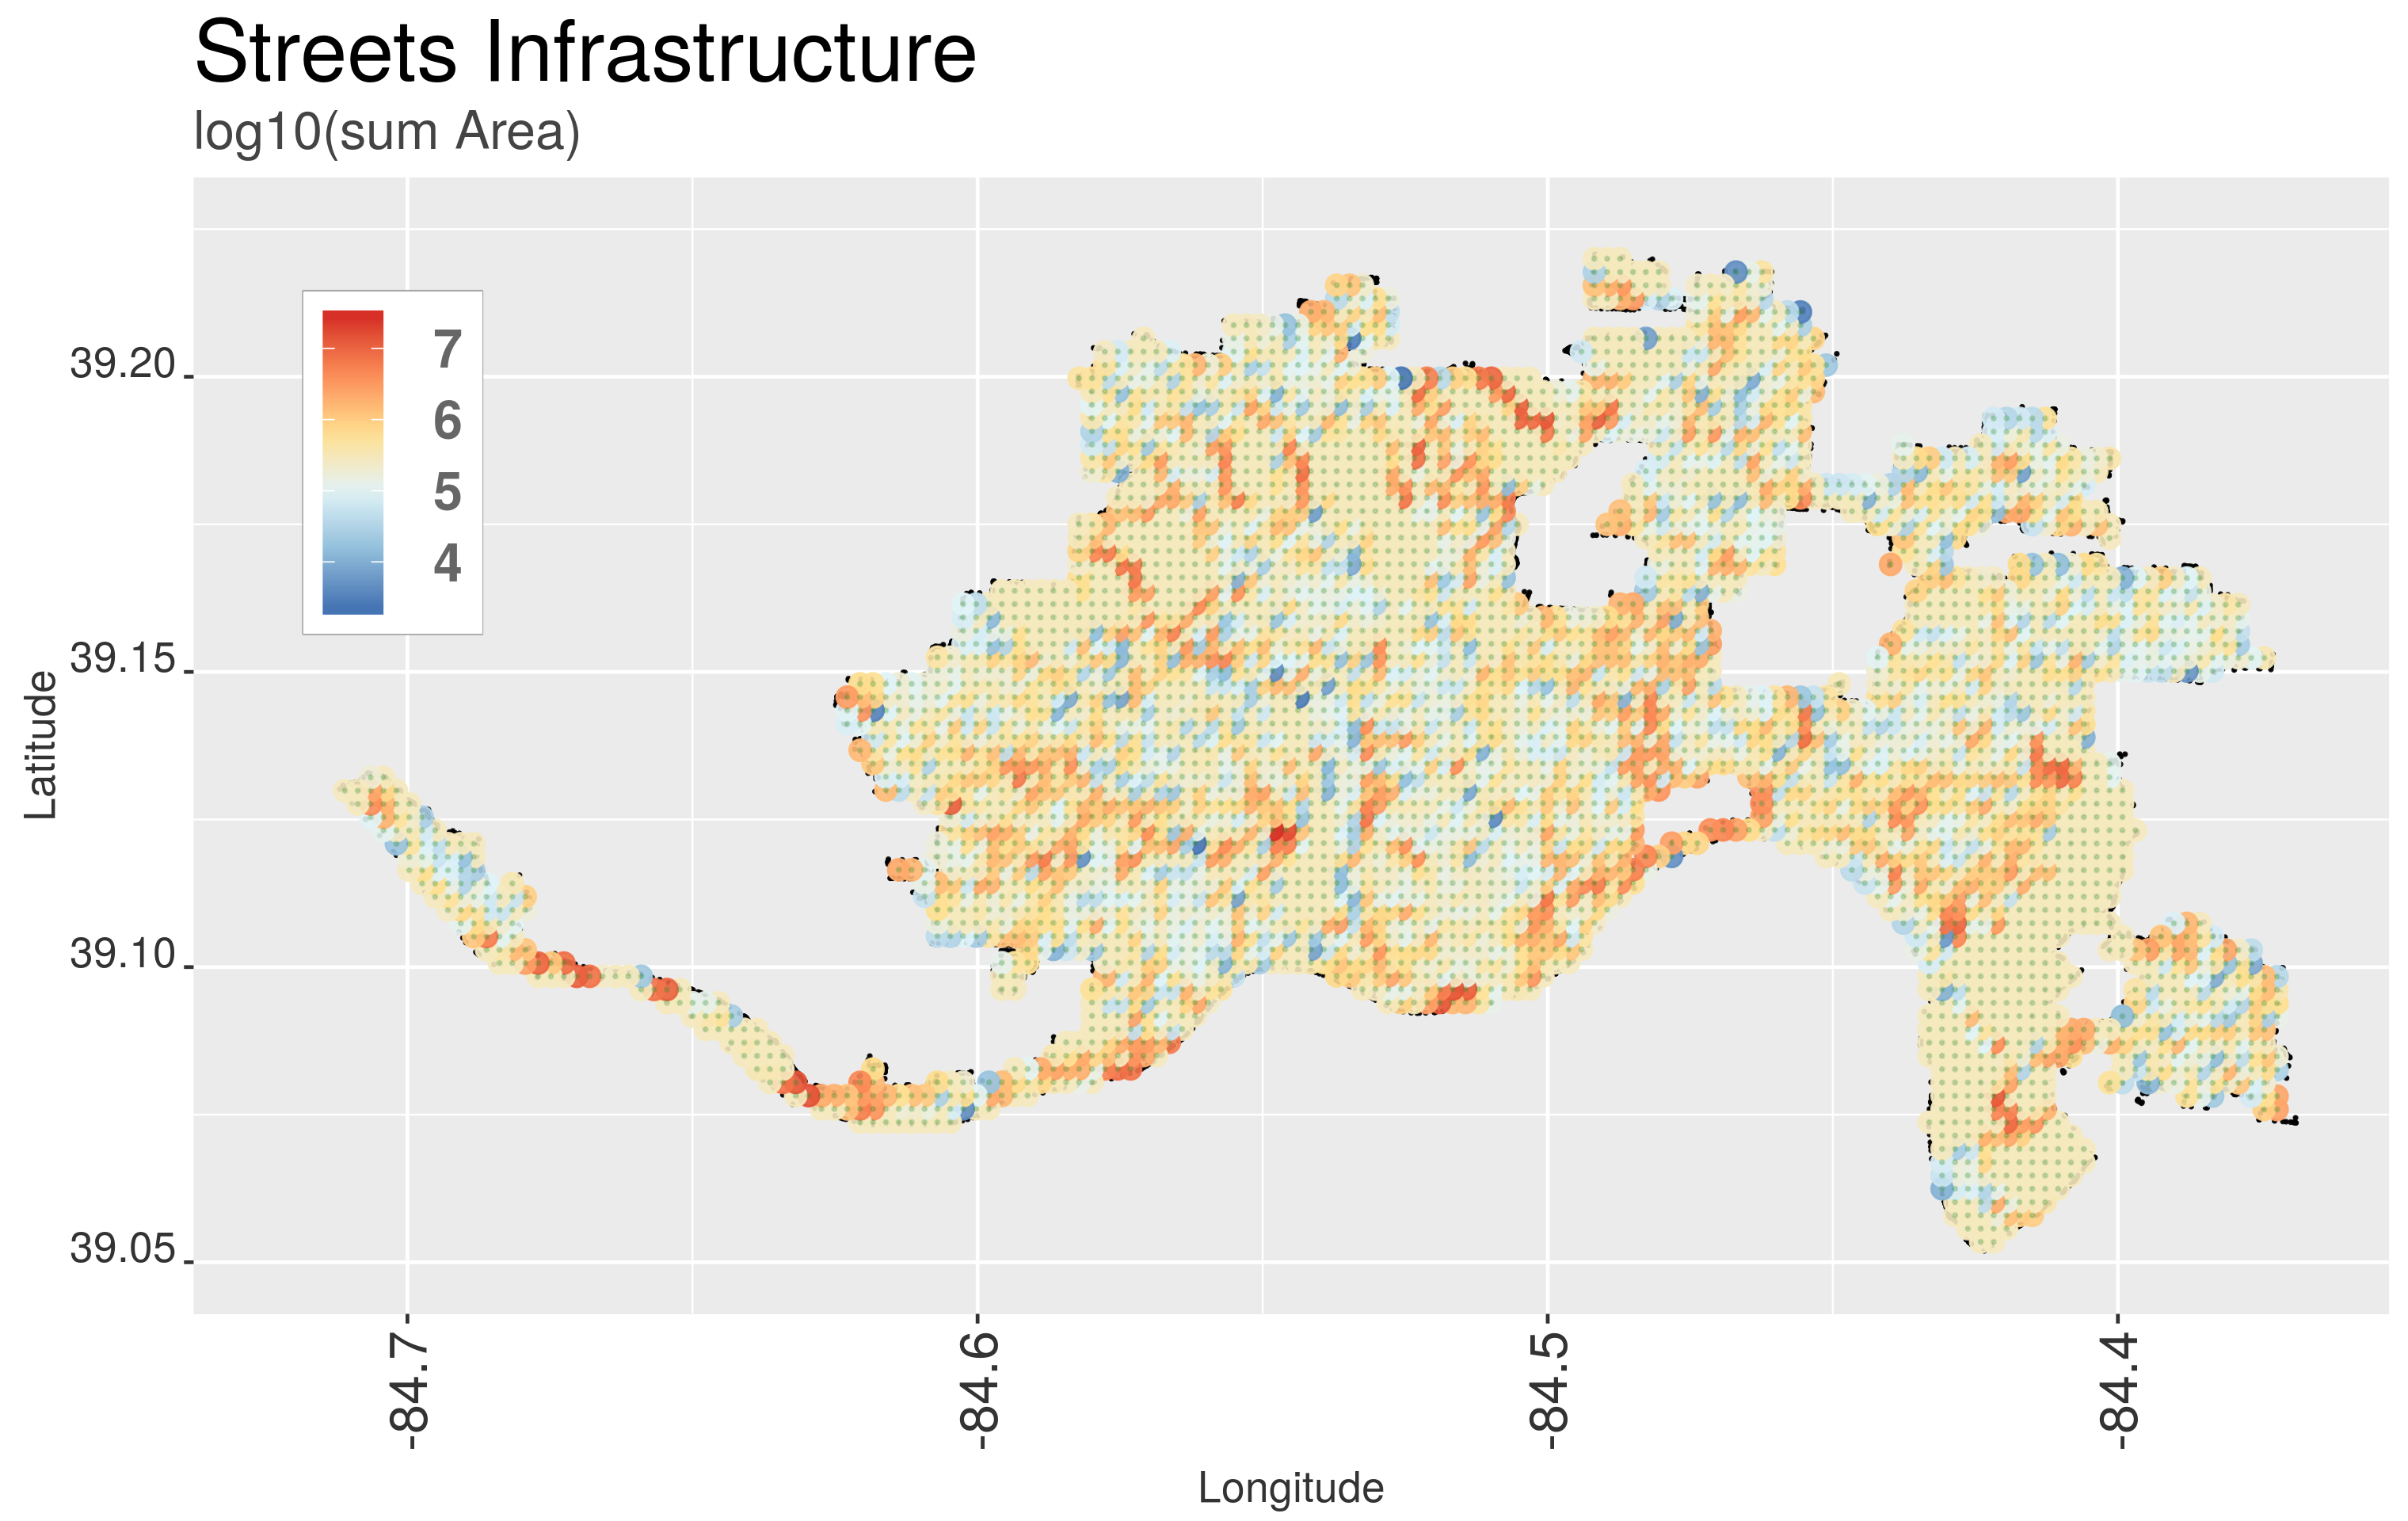
\includegraphics[width=\textwidth, height=\textheight, keepaspectratio]{streetsSumArea}
 	\caption{Streets - Sum of Surface Area}
	\label{figure : streetsSumArea}
\end{figure}
\FloatBarrier

% ...		---------------------------------------------------------------------------------------------------------

\subsubsection{Public Transportation}

The data set from the the Open Data Cincinnati portal  includes the location of every bus stop in the  Southwest Ohio Regional Transit Authority (SORTA) network. The SORTA bus network is the only public transportation network in the city. The data set includes 25,980 bus stops identified by latitude and longitude. We calculate the distance from every grid centroid to the nearest bus stop and use that value as a feature for the model. 

The distribution of the distances to nearest bus stop for this model are shown in Figure \ref{figure : busStopDistances}
% ... bus stop distances

\FloatBarrier
\begin{figure}
 	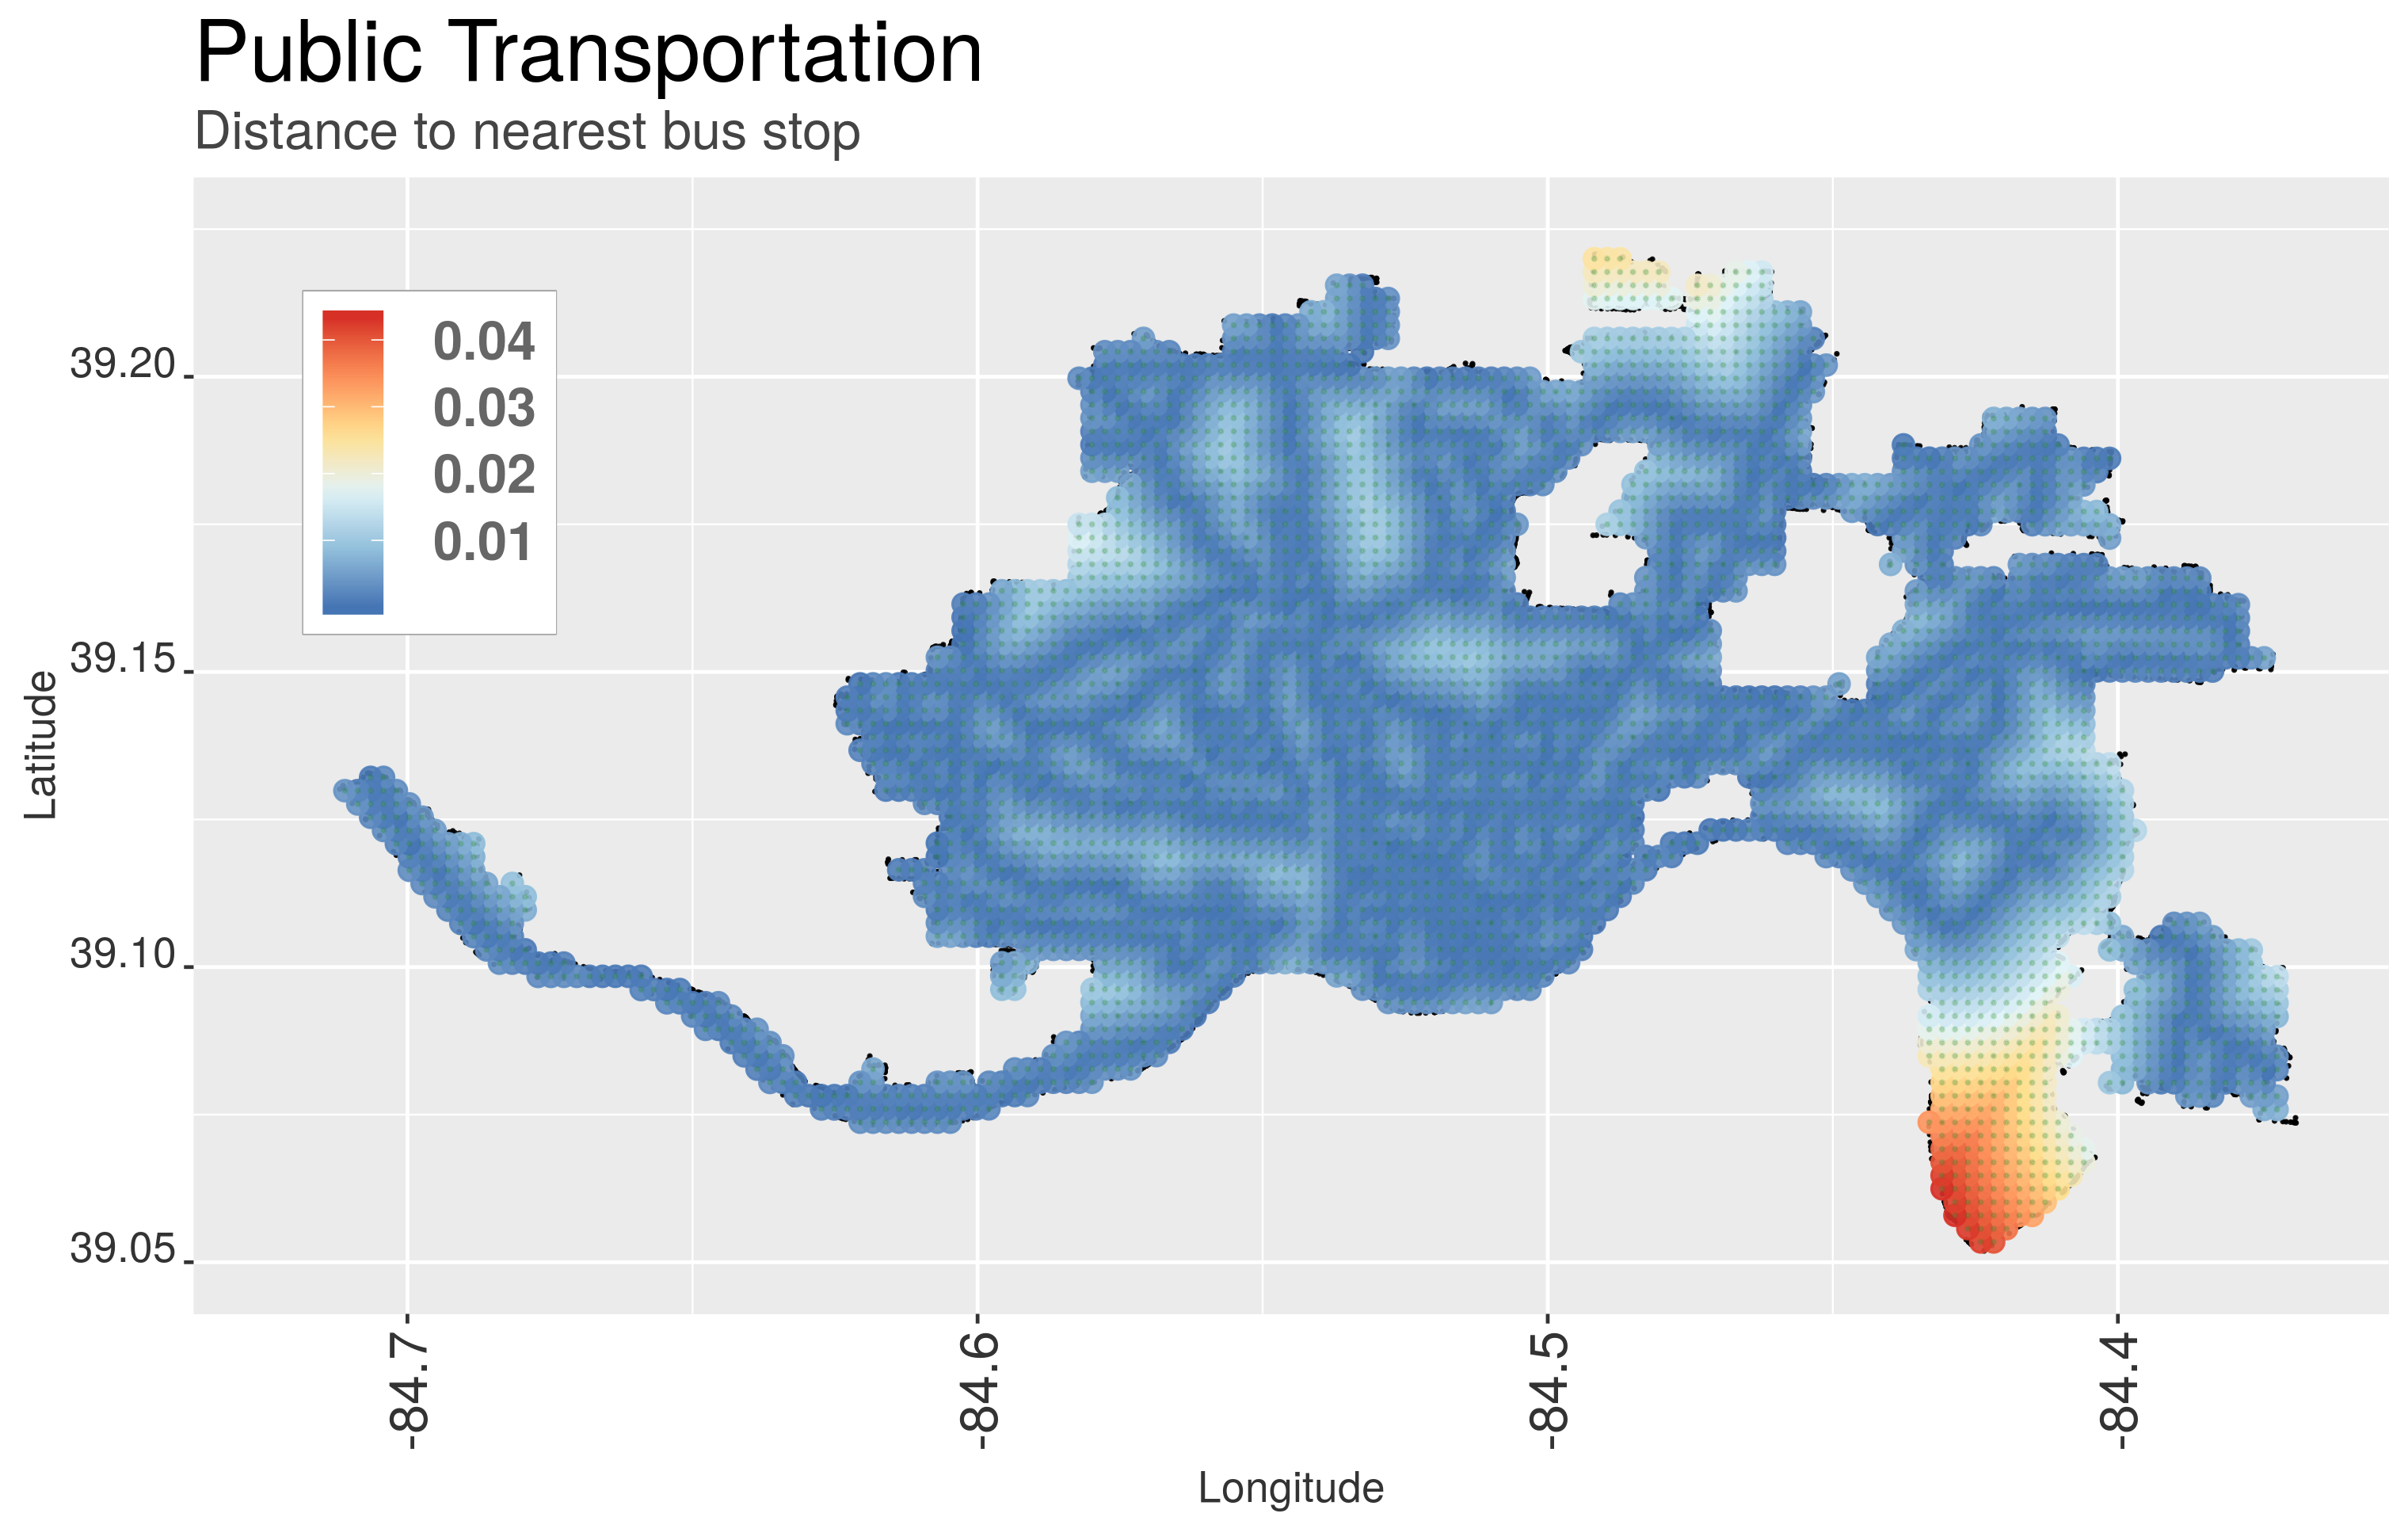
\includegraphics[width=\textwidth, height=\textheight, keepaspectratio]{busStopDistances}
 	\caption{Public Transportation Access}
	\label{figure : busStopDistances}
\end{figure}
\FloatBarrier

% ...		---------------------------------------------------------------------------------------------------------

\subsubsection{Non-Emergency request for service}

The data set from the the Open Data Cincinnati portal  includes a definition of every non-emergency request for service. These requests are initiated by the population and include a full range of services requested of city services.  There are 613,000 requests that were made  in the years 2012 through 2018. As a candidate independent feature characteristic for this model, we distribute each of the requests to the appropriate grid cell,  aggregate the number of requests in each major category and also the total number of requests. We do not apply a kernel function to distribute these requests over the local geographic region for the independent predictor features. The density of the actual experience is sufficiently distributed that a kernel function for density diffusion is not needed to achieve wide distribution and sufficient coverage for service request characterization among all of the grid cells. The distribution of the total number of requests per grid cell are shown Figure \ref{figure : nonEmergencyNumRequests}. The number of total requests that were recorded in each category are shown in Table \ref{table : nonEmergencyRequests}.

%

\FloatBarrier
\begin{table}[!h]
\begin{center}
\caption{Non-Emergency Service Requests (2012 - 2018)}
\label{table : nonEmergencyRequests}
\begin{tabular}{lr}
\hline
\rule{0pt}{12pt}
Request Type  	&	Number Requests	\\
\hline
Animals/Insects	&	7765	\\
Building Related	&	61616	\\
Construction	&	843	\\
Food	&	2153	\\
Others	&	171613	\\
Police Property	&	8546	\\
Service complaint	&	4374	\\
Street/Sidewalk	&	55555	\\
Traffic/Signal	&	1167	\\
Trash	&	272932	\\
Trees/Plants	&	22092	\\
Water Leak	&	1211	\\
Zoning/Parking	&	3132	\\
Number Total Requests	&	612999	\\[2pt]
\hline
\end{tabular}
\end{center}
\end{table}
\FloatBarrier


\FloatBarrier
\begin{figure}
 	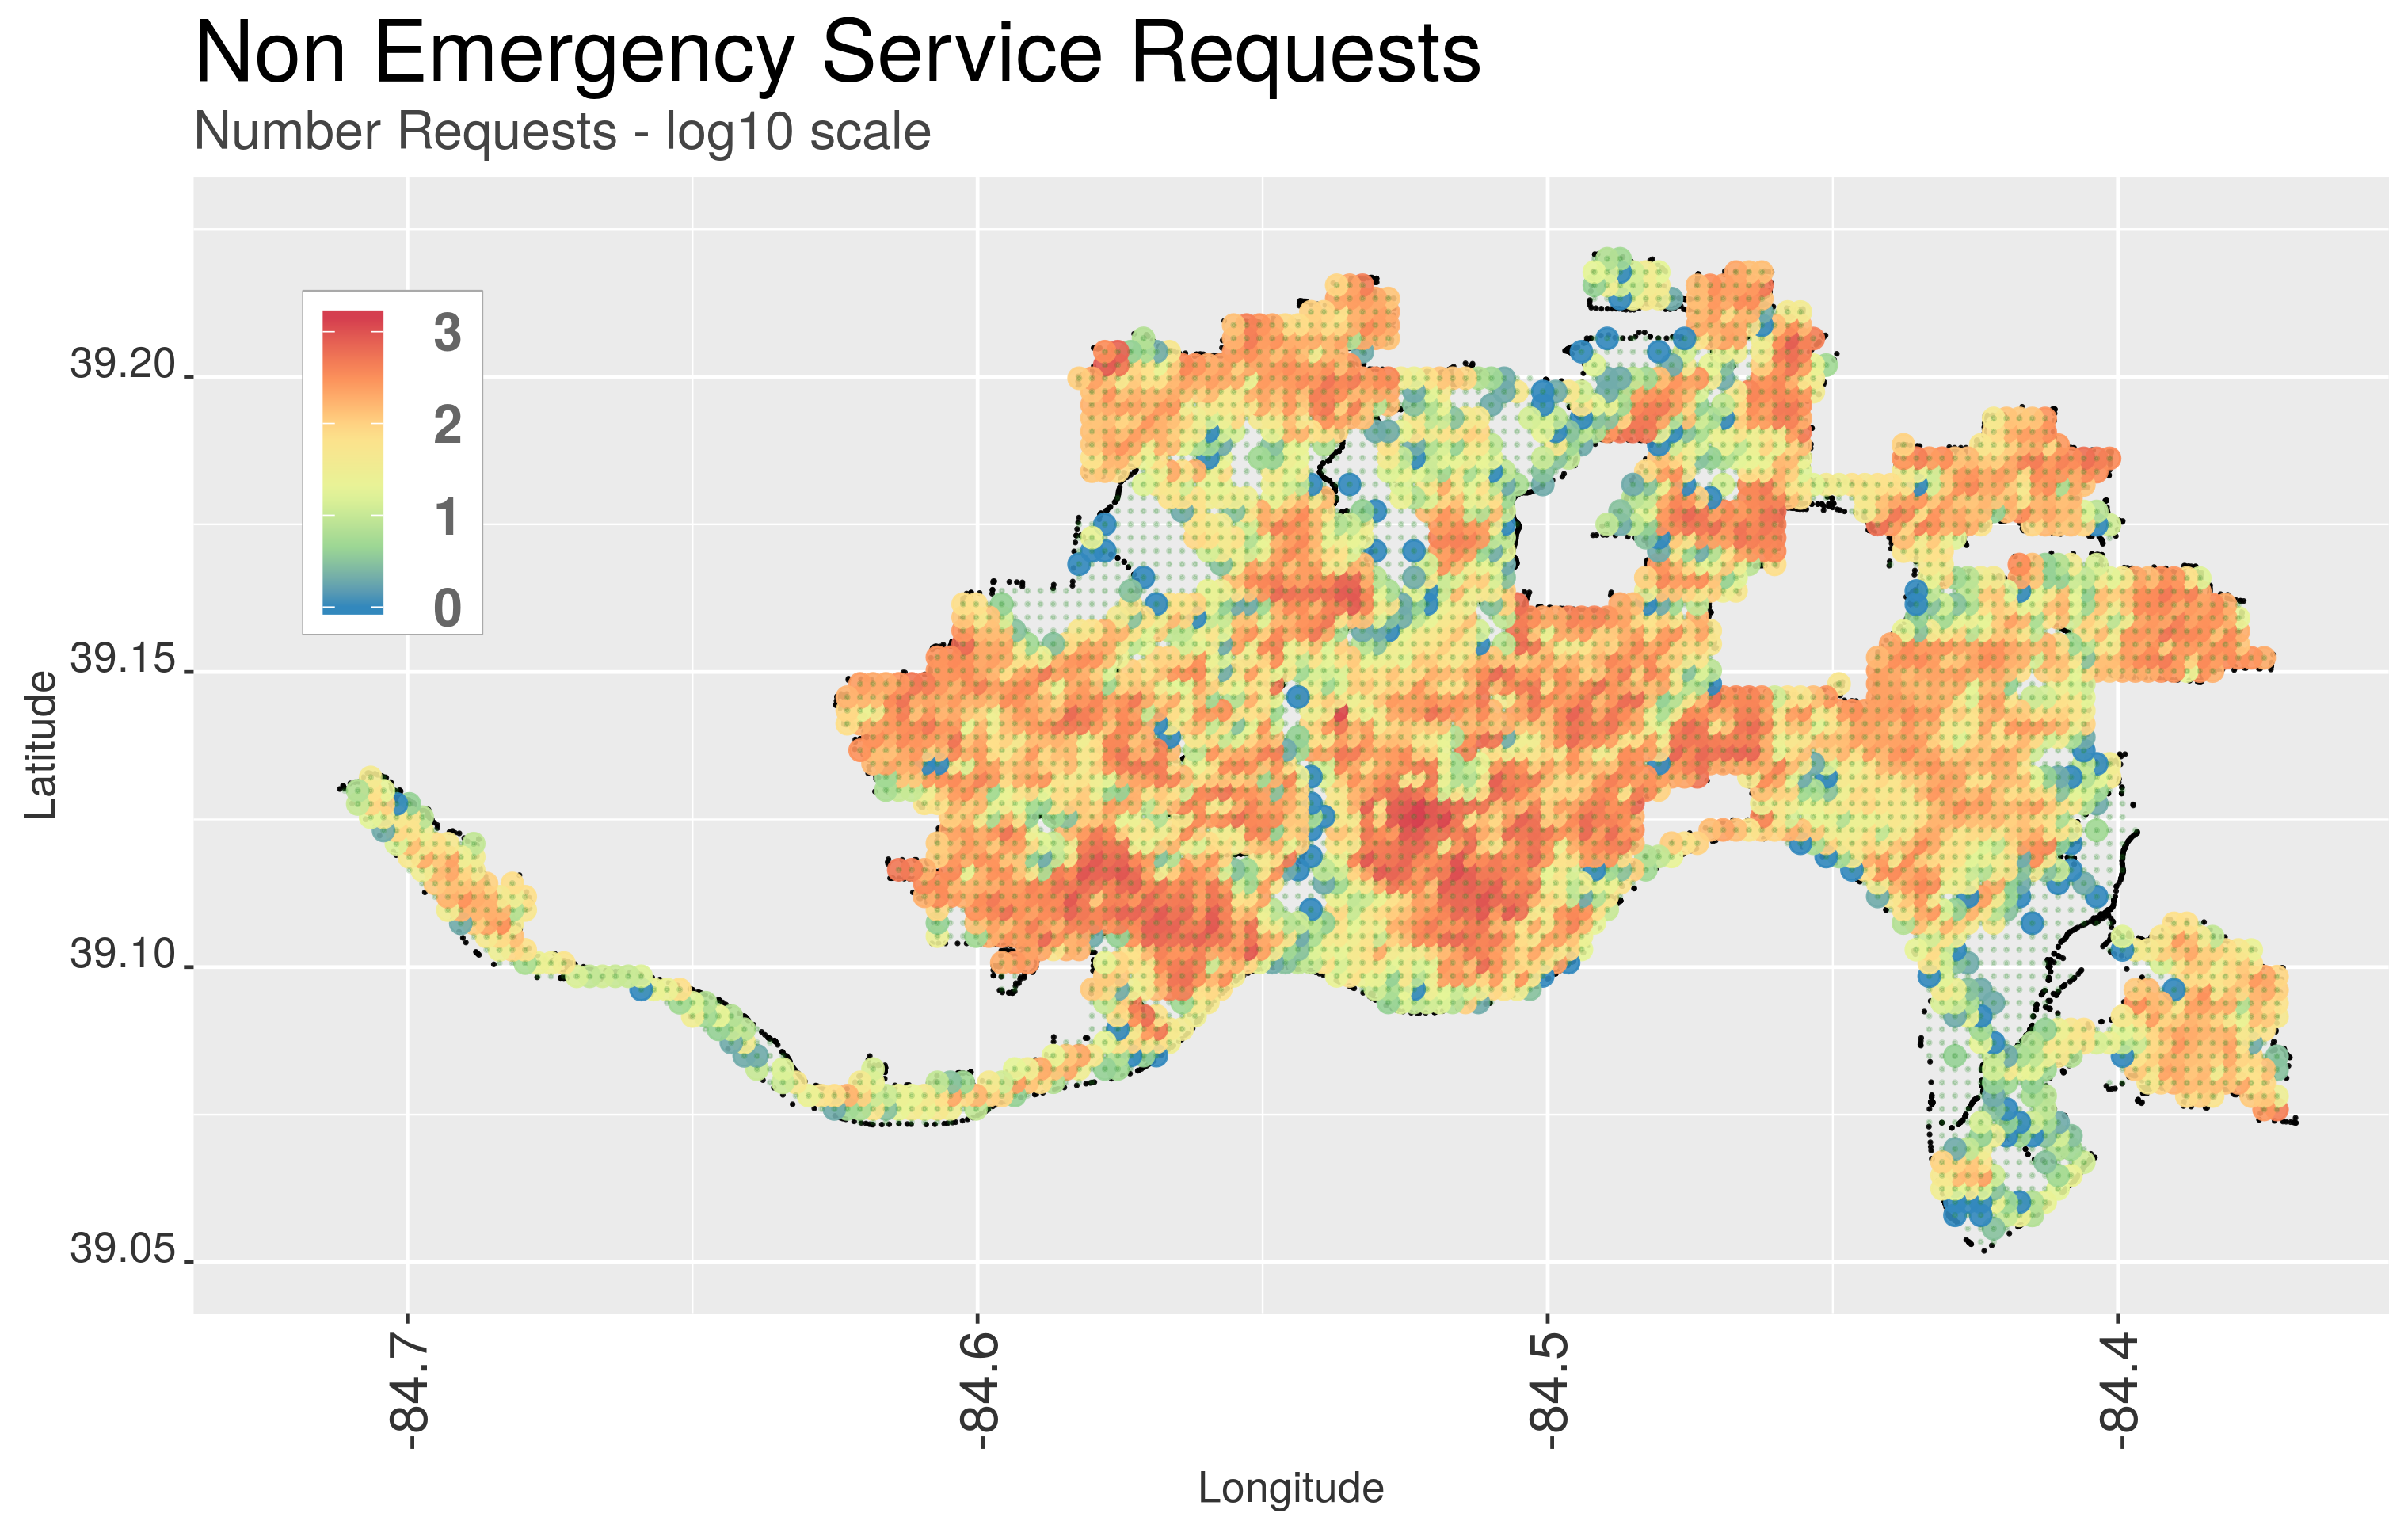
\includegraphics[width=\textwidth, height=\textheight, keepaspectratio]{nonEmergencyNumRequests}
 	\caption{Traffic Accidents - Non-Pedestrian}
	\label{figure : nonEmergencyNumRequests}
\end{figure}
\FloatBarrier

% ...		---------------------------------------------------------------------------------------------------------

\subsection{Cincinnati Pedestrian Survey}

As an avenue of data collection in response to the number of pedestrian accidents, the City of Cincinnati requested citizen input to identify specific areas in the city which are pedestrian safety concerns. The city created a web-site, which launched in Feb-2018 \cite{cvg2018city}, that allows citizens to specifically identify a location on a map, within a distance of several feet of the area of concern, and report the nature of the concern in a functional user interface. The user interface was available from Feb 2018 to April 2018\footnote{http://cagisonline.hamilton-co.org/pedsafetysurvey}. \cite{cvg2018city}. The survey screen provided users with view of the city, a drop down of neighborhoods, and a list of issue categories. The user then selected a neighborhood, and selects from the pre-defined issue types to report, and also has an opportunity to write a comment. If another citizen selects the same location and issue type, comments are appended as additional comments. This provides an idea of the number of users having same issue at a particular location. Survey submissions are anonymous. The city plans to use this community input to prioritize maintenance and improvement resources.

As candidate independent feature characteristics for this model, we distribute each registered concern type to the appropriate grid cell,  aggregate the number of registered concerns in each major category and also the total number of survey inputs. We do not apply a kernel function to distribute these over the local geographic region. The data features are shown in Table \ref{table : pedestrianSurvey}. 
An example of the distribution of the number of citizen inputs are shown in Figure \ref{figure : pedestrianSurveyNRequests}

% ... pedestrian survey

\FloatBarrier
\begin{table}[ht]
\begin{center}
\caption{Pedestrian Survey - Citizen Input}
\label{table : pedestrianSurvey}
\begin{tabular}{clr}
%{ p{0.3\textwidth} p{0.6\textwidth}}
\hline
%\rule{0pt}{12pt}
Category	&	Description & Number			\\
\hline
\multirow{15}{*} {Concern type}	&	{Accessibility issue}	&	35	\\
		& Crosswalk Needed	&	311	\\
		&Double Parking	&	52	\\
		&Jaywalking	&	141	\\
		&Lack of Visibility	&	210	\\
		&Long wait for walk signal	&	54	\\
		&No Bike Facilities	&	58	\\
		&No Sidewalks	&	247	\\
		&Other	&	448	\\
		&Parking on the sidewalk	&	112	\\
		&Parking too close to intersection	&	127	\\
		&Speeding	&	977	\\
		&Vehicles do not yield at crosswalks	&	515	\\
		&Vehicles run red lights or stop signs	&	443	\\
		&Walk signal is too short	&	57	\\
		&Total number concerns &  3787 \\
\hline
\multirow{5}{*} {User type}	&	bikes	&	154	\\
		&drives	&	1152	\\
		&{travels (other)}	&	186	\\
		&uses an assistive device	&	66	\\
		&walks	&	2229	\\[2pt]
\hline
\end{tabular}
\end{center}
\end{table}
\FloatBarrier

%
% ... Pedestrian survey - number requests

\FloatBarrier
\begin{figure}
 	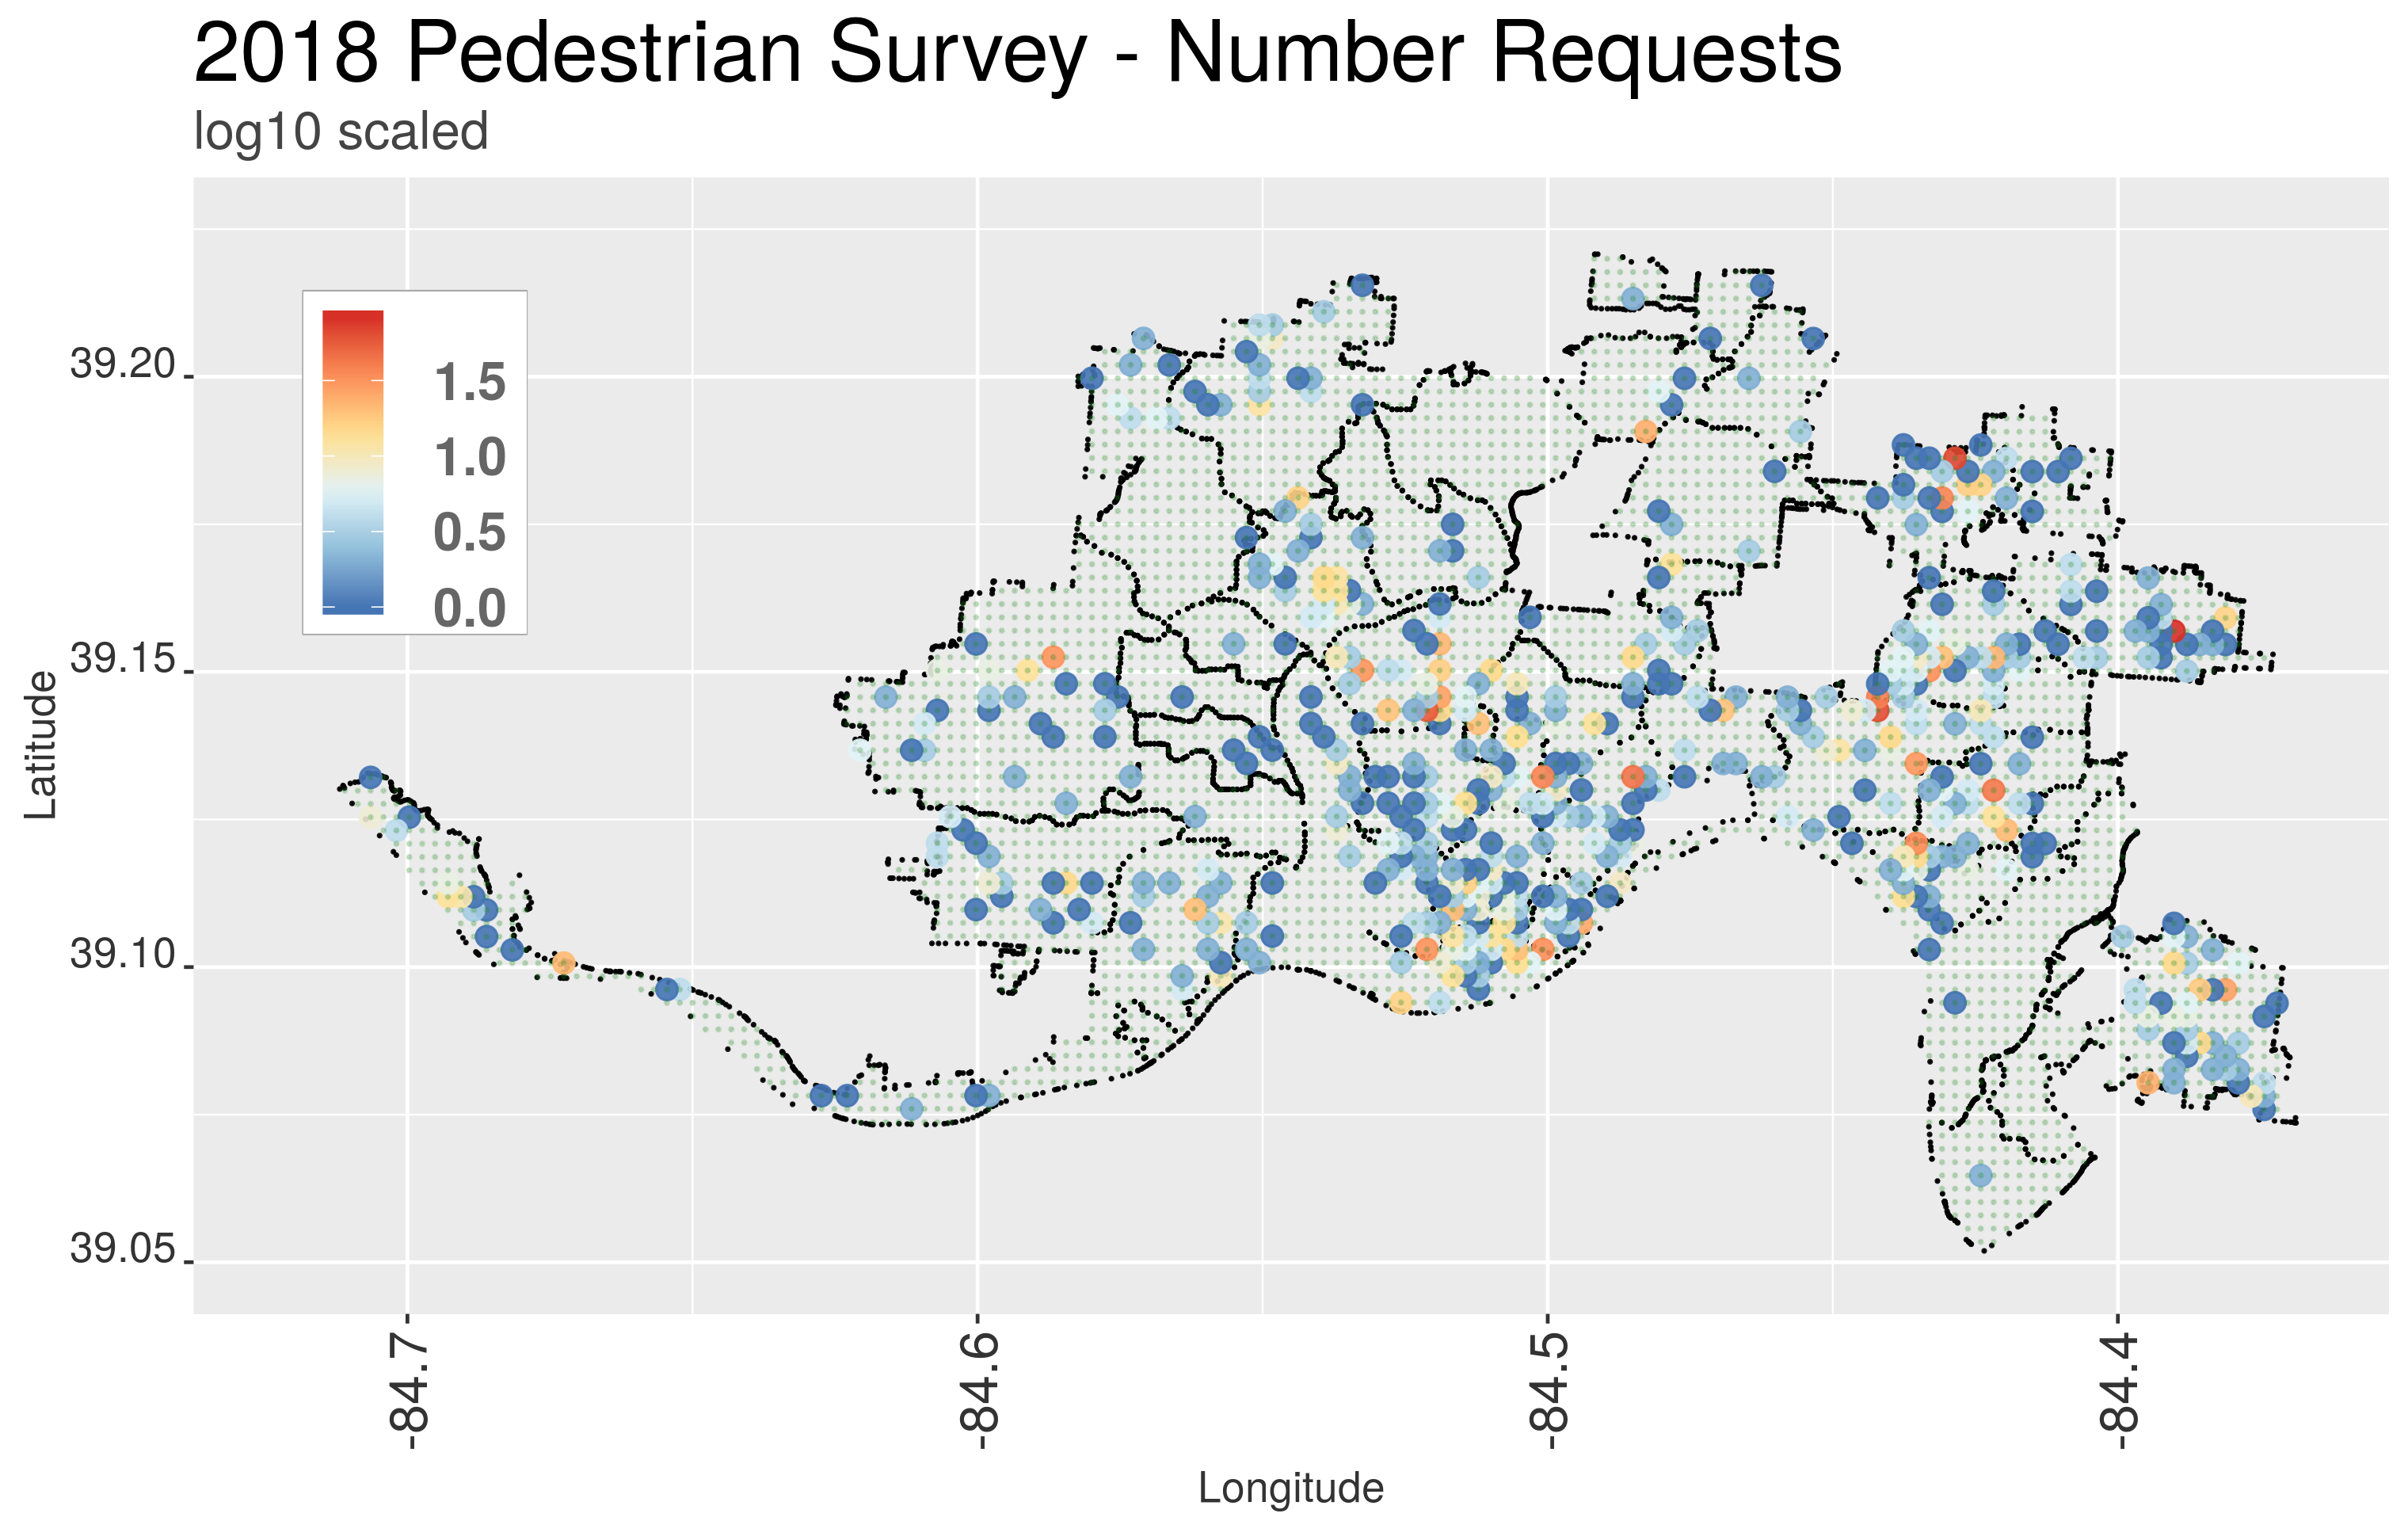
\includegraphics[width=\textwidth, height=\textheight, keepaspectratio]{pedestrianSurveyNRequests}
 	\caption{Median Property Values}
	\label{figure : pedestrianSurveyNRequests}
\end{figure}
\FloatBarrier

% ...		-=-=-=-=-=-=-=-=-=-=-=-=-=-=-=-=-=-=-=-=-=-=-=-=-=-=-=-=-=-=-=-=-=-=-=-=

\subsection{Neighborhoods}

For some elements of this project we relied on descriptions of neighborhoods, neighborhood boundaries, and real estate market valuation. To support those elements we used data sources available from Zillow. Zillow is an on-line real estate based service providing information about residential properties for sale, for rent, or recently sold\footnote{https://www.zillow.com/}. Zillow provides on-line access to real estate information and services to consumers. A part of the resources made available by Zillow are neighborhood boundary shapefiles. These files are shared under a Creative Commons license, allowing freedom to use the data sets provided attribution is made to Zillow. For our purposes, we used the neighborhood boundaries for three purposes. First, the neighborhood boundary shapefiles for the City of Cincinnati were used to identify grid cells and experiences that were strictly within the boundaries of the city using the latitude and longitude coordinates of the shapefiles. In addition, each grid cell in the model was attributed to one of the forty-six neighborhoods included in the Zillow defined boundaries. These neighborhood assignments were then used to support imputation for grid cells that had missing values for property value information. The grid cells without property value assignment were imputed using median values within a neighborhood. Additionally, the neighborhood boundaries were used following the unsupervised learning to differentiate clustering analysis results in the context of named neighborhoods. We observe that the Zillow neighborhood definitions include two neighborhoods, Fruit Hill and Forestville, on the eastern boundary of the city which are not, in fact, within the city incorporation limits. We dropped those neighborhoods from our model. An additional resource that we use from Zillow is the Cincinnati Market Overview, which provides an aggregate relative change in market valuation for the Cincinnati residential market for the years 2008 through 2018.  In the next section we describe the property valuation information that we use in our model that is acquired from the Hamilton County (OH) Auditor. We adjust the historical information from that source using the relative market valuation change that is available from the Zillow web-site. The relative values are shown in Table \ref{table : marketappreciation}.

\FloatBarrier
\begin{table}[!h]
\begin{center}
\caption{Cincinnati Residential Market Appreciation}
\label{table : marketappreciation}
\begin{tabular}{lrr}
\hline
\rule{0pt}{12pt}
Year	&	Median Value (\$K)	&	Adjusted to 2018 (percent)	\\
2008	&	113	&	1.13	\\
2009	&	113	&	1.13	\\
2010	&	103	&	1.24	\\
2011	&	100	&	1.28	\\
2012	&	99	&	1.29	\\
2013	&	98	&	1.31	\\
2014	&	99	&	1.29	\\
2015	&	100	&	1.28	\\
2016	&	111	&	1.15	\\
2017	&	115	&	1.11	\\
2018	&	128	&	1.00	\\[2pt]
\hline
\end{tabular}
\end{center}
\end{table}
\FloatBarrier
%

% ...		-=-=-=-=-=-=-=-=-=-=-=-=-=-=-=-=-=-=-=-=-=-=-=-=-=-=-=-=-=-=-=-=-=-=-=-=

\subsection{Property Valuation}

Cincinnati is located within Hamilton County (OH). The Hamilton County Auditor provides access to data files that describe the property transfers that have occurred in the county via their web-site\footnote{\label{hcauditor}www.hamiltoncountyauditor.org}. We use the last 10 years (2008 through 2018) property transfers as a means to identify local property values. Each property transfer which takes place includes descriptive information such as : property address, transfer date, type of property (residential, commercial, industrial, publicly-owned), binary flag to indicate if property transfer is considered valid (i.e., open market sale or not). For each property transfer, we use the property address information to identify the geo-coordinates for subsequent mapping to appropriate grid cell and identify the properties that are within the City of Cincinnati incorporation limits by superposition with the neighborhood shapefile as described in the preceding section. In addition, we value adjusted each transfer, based on year of sale, using the market valuation adjustments shown in Table  \ref{table : marketappreciation}. Finally, we aggregate all property transfers within a grid cell and create the data features shown in Table \ref{table : propertyValueFeatures} 

% ... property value data features

\FloatBarrier
\begin{table}[!h]
\begin{center}
\caption{Property Value Features}
\label{table : propertyValueFeatures}
\begin{tabular}{ p{0.9\textwidth}}
\hline
\rule{0pt}{12pt}
Data Feature	\\
\hline
Median sale price – residential – valid sale\\
Median sale price – residential – non-valid sale\\
Median sale price – commercial – valid sale\\
Median sale price – commercial – non-valid sale\\
Median sale price – industrial – valid sale\\
Median sale price – industrial – non-valid sale\\
Median sale price – public owned – valid sale\\
Median sale price – public owned – non-valid sale \\[2pt]
\hline
\end{tabular}
\end{center}
\end{table}
\FloatBarrier
%

An example of the distribution of the property values for this model are shown in Figure \ref{figure : medianpropertyvalues}

% ... Median residential property values
\FloatBarrier
\begin{figure}
 	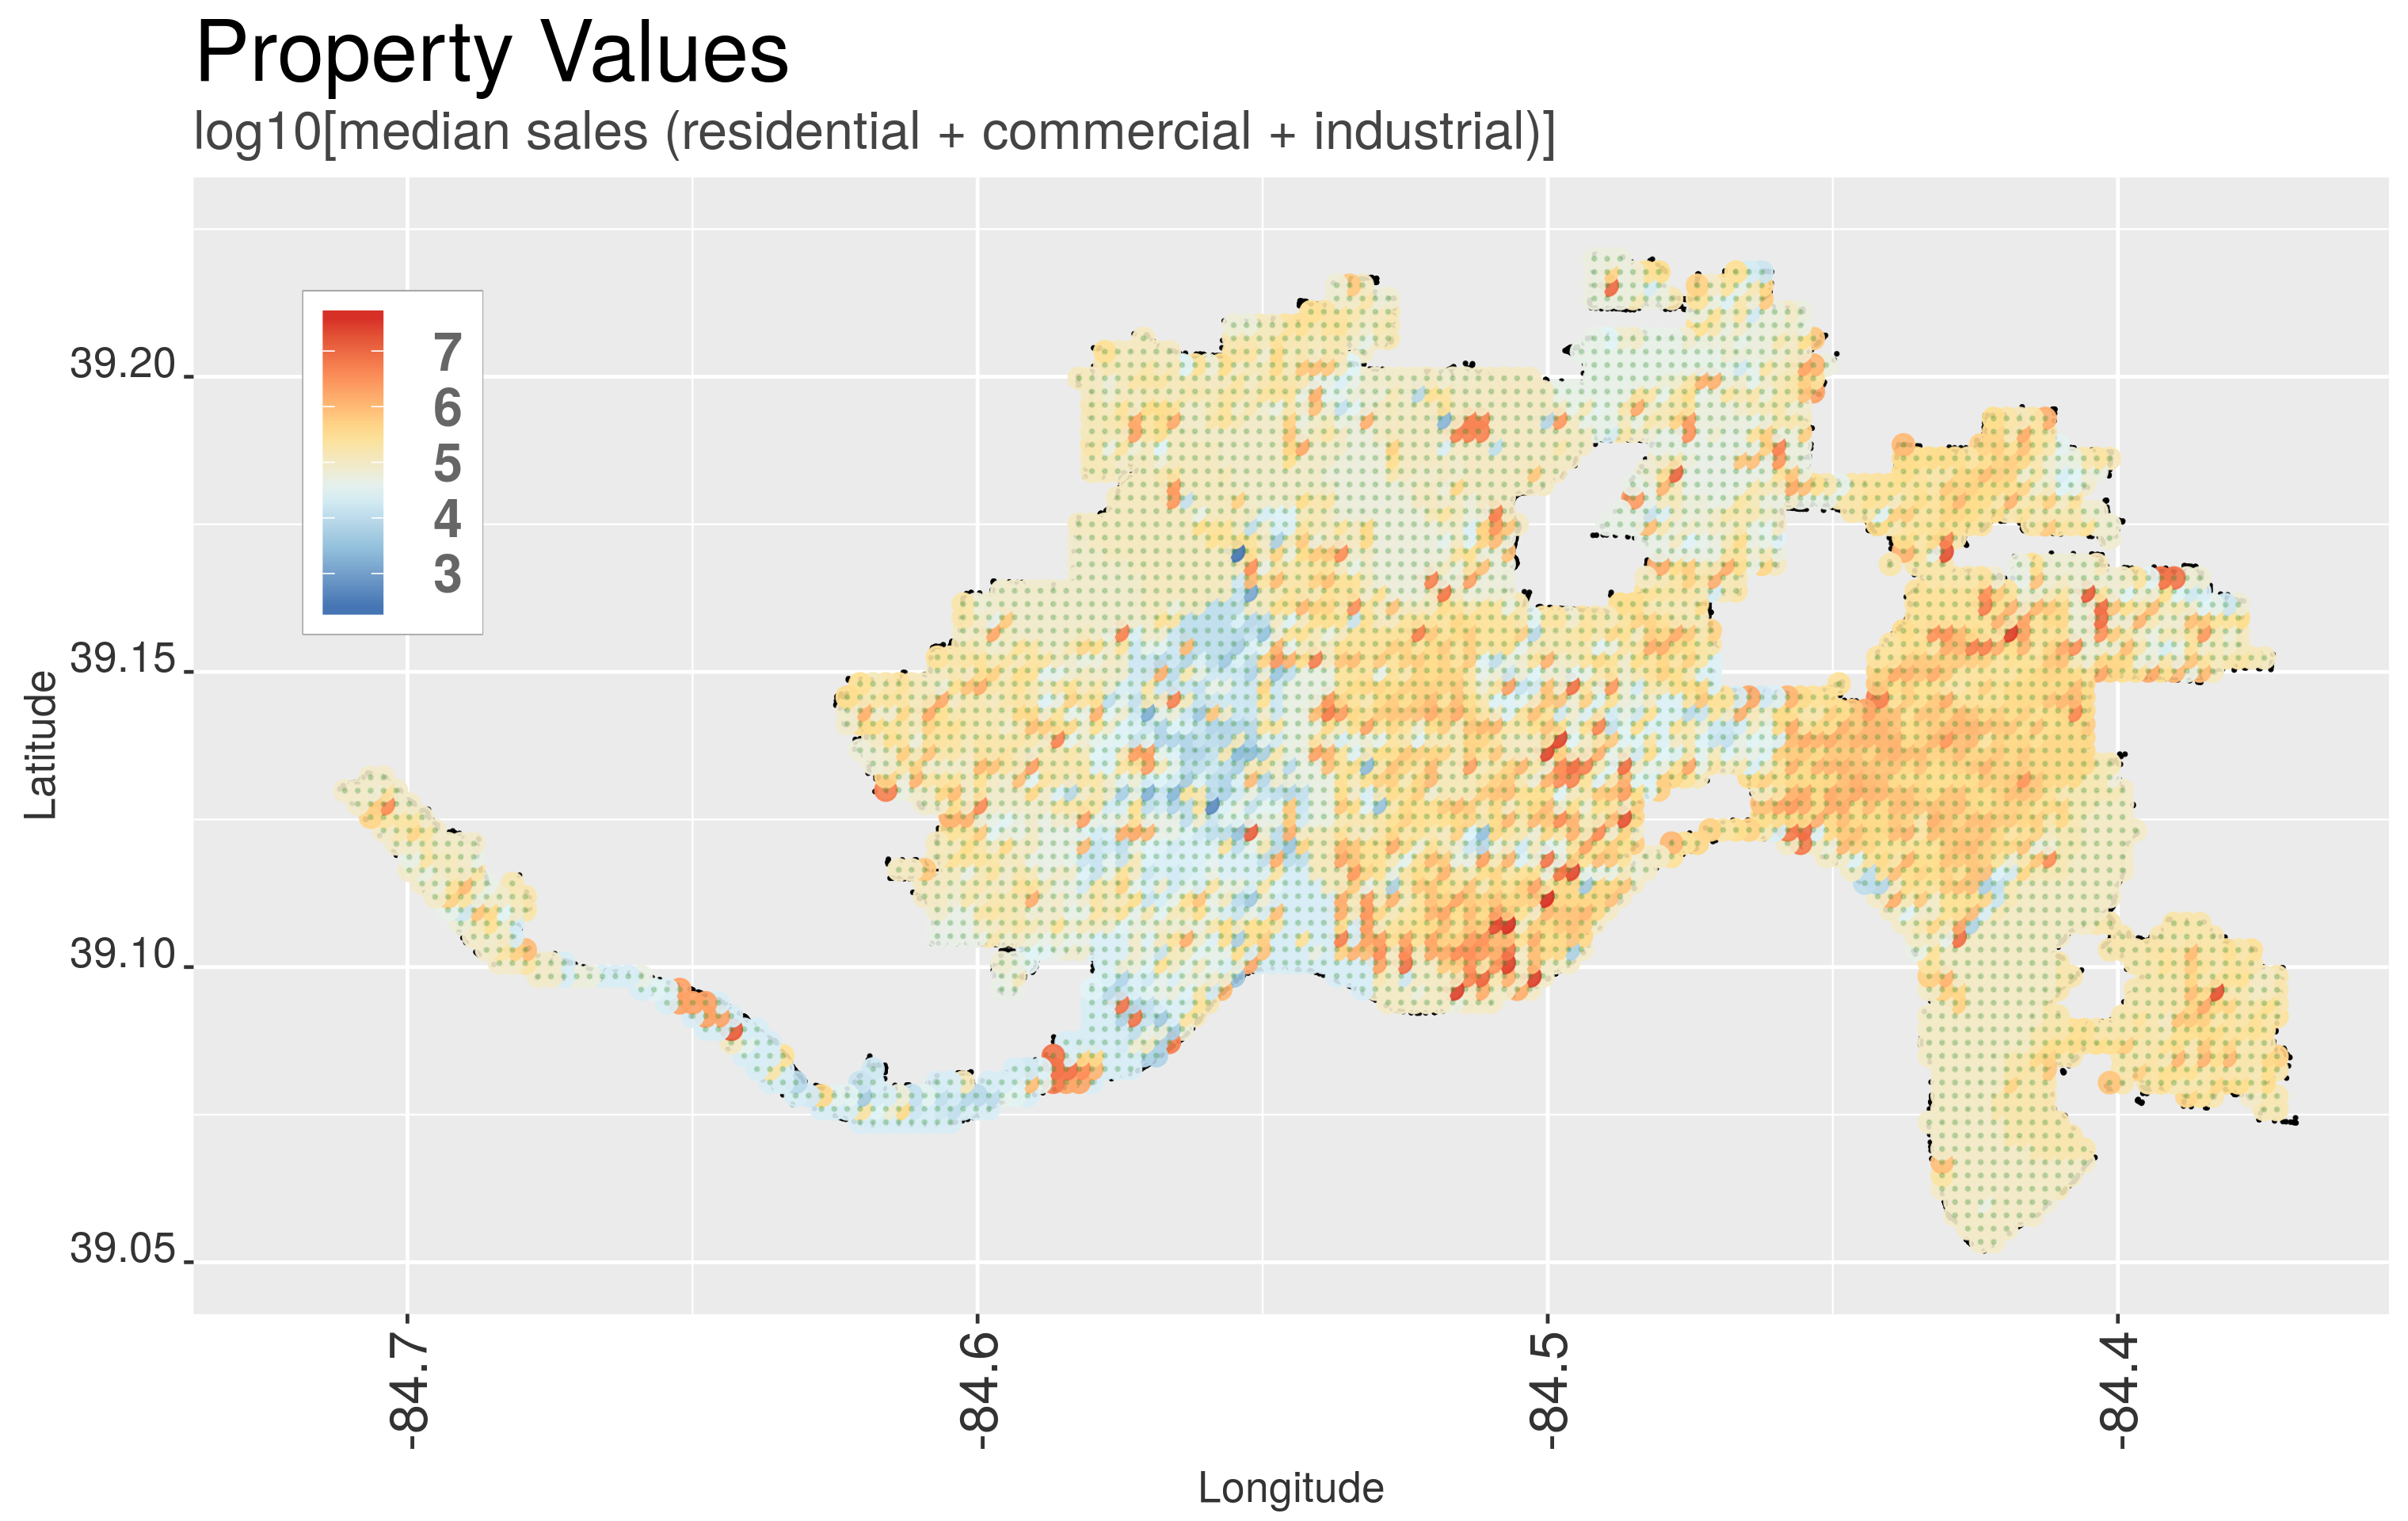
\includegraphics[width=\textwidth, height=\textheight, keepaspectratio]{propertyValuesMedianAllY}
 	\caption{Median Property Values}
	\label{figure : medianpropertyvalues}
\end{figure}
\FloatBarrier

% ...		-=-=-=-=-=-=-=-=-=-=-=-=-=-=-=-=-=-=-=-=-=-=-=-=-=-=-=-=-=-=-=-=-=-=-=-=

\subsection{Walk Score\textsuperscript{\tiny\textregistered}}

Additionally, the date of the issue created, typical mode of user (walk, drive, bicycle), and intersection of the location selected are captured. There are 3788 records in our survey dataset with 8 usable columns. There are missing data and categorical data in incorrect format which require clean-up and updating of missing information. Other than the survey data, we have various sources of data which would be combined to form the dataset for the project. All acquired from the City of Cincinnati are listed in Table ~\ref{table:cincinnatidatasets}. Datasets that originated from the Open Data Cincinnati are listed in Table ~\ref{table:cincinnatiopendata}.  Supplementary data sets from external sources are listed in Table ~\ref{table:supplementarydatasets}.

An example of the distribution of the property values for this model are shown in Figure \ref{figure : walkScore}

% ... Median residential property values
\FloatBarrier
\begin{figure}
 	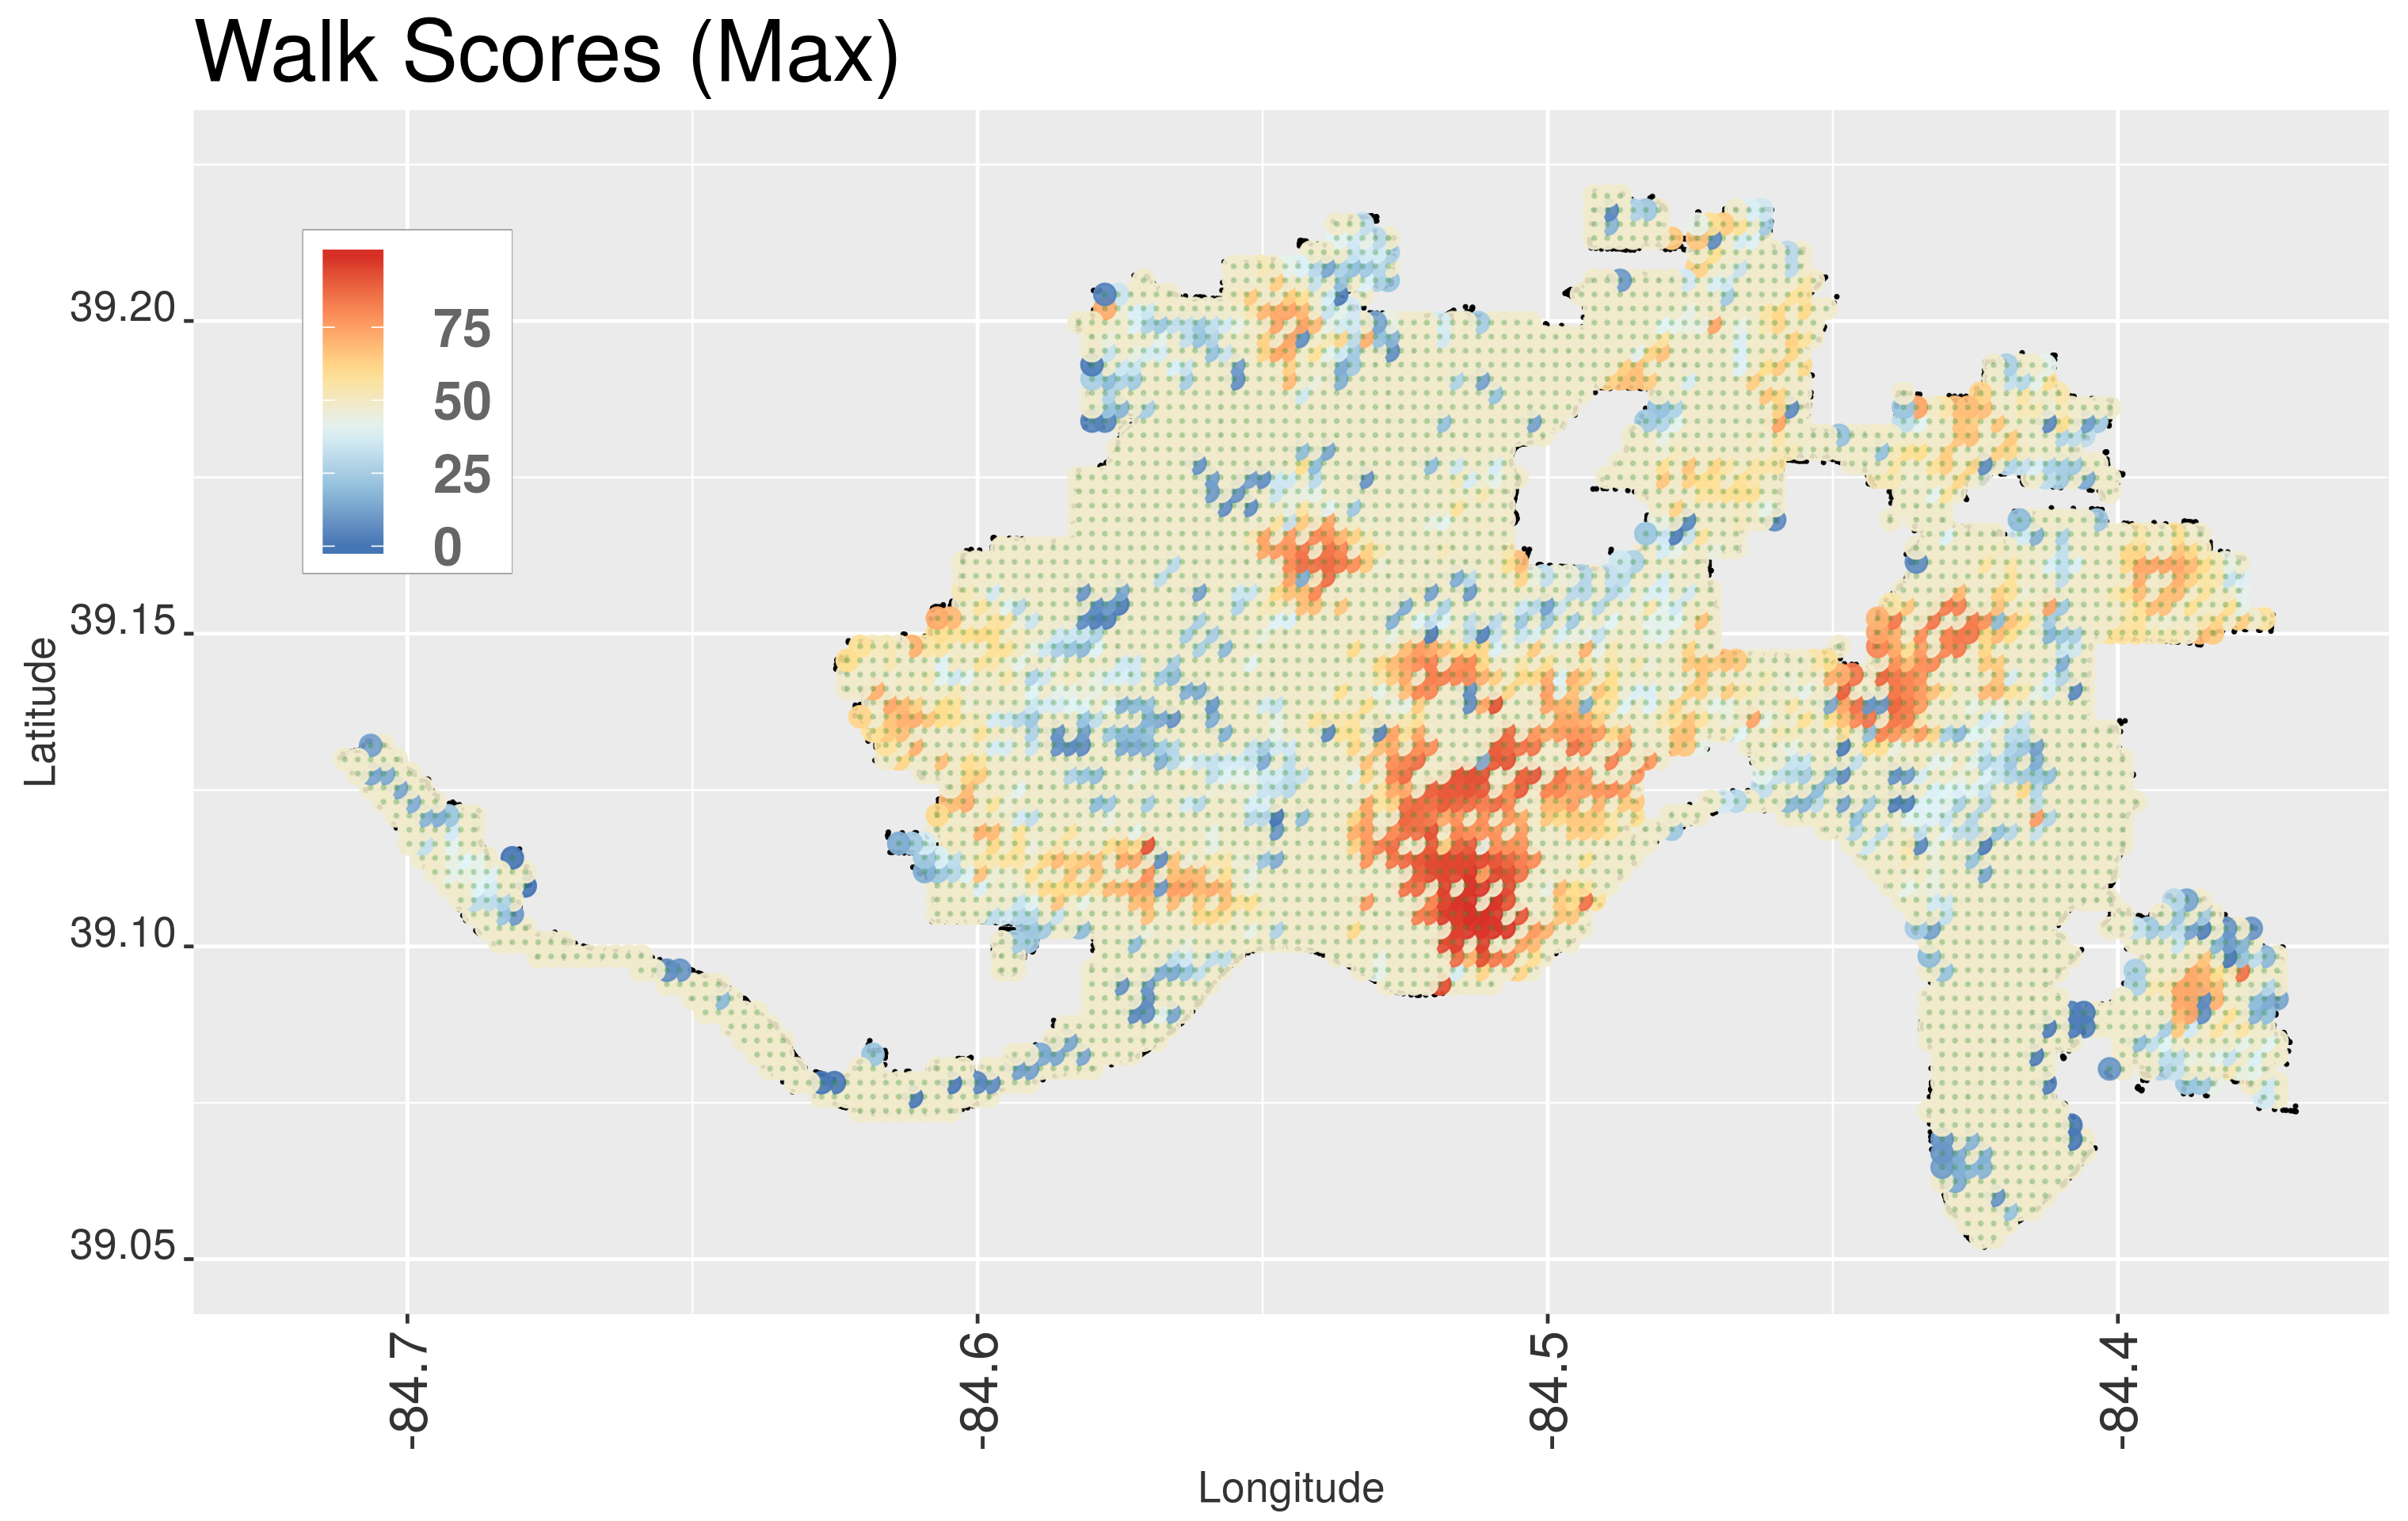
\includegraphics[width=\textwidth, height=\textheight, keepaspectratio]{walkScore}
 	\caption{Walk Score\textsuperscript{\tiny\textregistered} distributed values}
	\label{figure : walkScore}
\end{figure}
\FloatBarrier

\section{Methods and Experiments}
% ...		-=-=-=-=-=-=-=-=-=-=-=-=-=-=-=-=-=-=-=-=-=-=-=-=-=-=-=-=-=-=-=-=-=-=-=-=

As identified in the discussion around Figure \ref{figure : PedestrianCosts}, the bifurcated distribution of cost severity as distributed among the grid cells encourages the idea to develop a two-part model for the supervised learning element of this evaluation. We consider the two-part model as (a) develop a binary estimator to model the presence / absence of pedestrian accident costs, and (b) for the positive case of (a), develop an estimator of the magnitude of the cost severity function.

We consider two possibilities for the binary estimator : (a) binary logistic regression model, and (b) a random forest model. In both cases, we assess the capability to estimate the absence (no cost) and presence (cost $>$ 0).

As the second step in the two-part model, we use a multi-variate OLS regression model (on the log-transformed costs) to provide estimation of the expected cost for the case that the cost is greater than zero. The description of this two-part model is expressed in the following relation : 
% 
\begin{align}
E[Y| X] &= \Pr(Y > 0 | X)\times E(Y | Y > 0,  X).
\end{align}


%
\subsection{Data Ingestion and Grid Aggregation}


Initial results from part 1 of our methodology have produced graphs as shown in Figure ~\ref{figure:SumCrashPlot}. \newline

\FloatBarrier
\begin{figure}
 	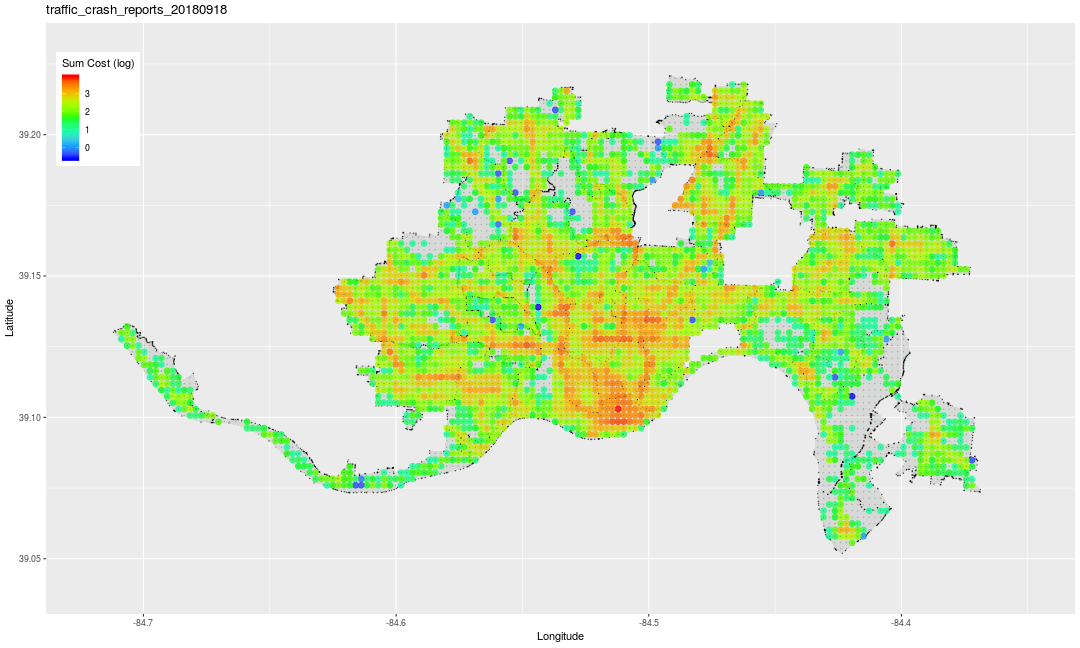
\includegraphics[width=\textwidth, height=\textheight, keepaspectratio]{trafficcrashreports20180918nonpedestriansumcostmapped2grid.png}
 	\caption{Sum cost of traffic crashes reported from 2012 to October 2018 involving pedestrians by grid cells.}
	\label{figure:SumCrashPlot}

\end{figure}
\FloatBarrier

\subsection{Random Forest - Binary Model}

\subsection{Multi-Variate Linear Regression - Cost Model}
In order to create a linear cost model to predict the cost of a PVI, the data must lend itself to the assumptions of a parametric model. These assumptions include normality, linearity, constant variance, and independence. The response variable within the data has a very abnormal distribution, with nearly 80\% of the grid-cells containing no incidents of PVI and having 0 cost associated with them. This positively skewed data does not meet the assumption of normality even after multiple types of transformations, notably including the logarithmic transformation. In order to meet the assumption of normally distributed data, the data is subset to exclude locations where there is no data, and the few events resulting in extreme damage of \$5 million or more. This data subset dramatically reduces the skewness present in the dataset, and allows for linear regression modelling to proceed.

The reduced scope dataset is first run through the 10-fold cross validated stepwise selection of the caret package in R, in order to determine the best full model, ranging from 10 to 35 predictor variables. The function iterates through each number of predictor variables from 10 to 35, performing stepwise 10-fold cross validation for each number of maximum predictor variables. The 10-fold cross validation is a model validation technique used to reduce overfitting and promote the generalizability of the model. Model overfitting can occur when a model is trained on a particular dataset to the degree that it performs extraordinarily well in predicting on the dataset, but it fails to achieve that same level of prediction capability on other datasets. The parameters in an overly fit model do not generalize to the population at large because they are fine tuned to only reflect the dataset on which they were trained. The 10-fold cross validation splits the data into 10 pieces. In each of the 10 iterations, one is selected to be the testing dataset, and the other 9 are used to train the model. This methodology is repeated so that each of the 10 pieces has a chance to be the testing dataset. The result of these 10 trials are averaged and compared against the cross validation results at each other maximum variable value from 10 to 35. The full model chosen is the model with the lowest average root mean square error value, and in our study, was determined to be the model with 30 variables.

Once the full model is selected, it is then manually pruned based on the variance inflation factor values and significance. Variance inflation factor values larger than 5 signify collinearity between variables, and a violation of one of the parametric assumptions in linear regression. Variable significance is determined by the p-value, and the typical value used is .05. Variables at or below the .05 p-value threshold are determined to be statistically significant to the model, while those above it are not. In spite of this black and white view on p-values, some variables are left in the model which are not significant at the .05 level, but are suggestive of being significant influences to the model, as shown in Table ~\ref{table:RegressionAnalysis}. 

With the reduced model, the cost of non-fatality incidents to pedestrians is predicted for each event, and the resulting prediction is compared against the actual cost of incident. The difference between the predicted and actual cost is the residual, and the residuals are then mapped back to the Cincinnati map to visualize areas with potential for safety improvement.

\subsection{Unsupervised Learning - Neighborhood Characterization}

To develop the models in a way that supports an assessment of the generalizability of the models,  the dataset is shuffle split into 80:20, 20\% holdout for cross-validation, using the 10-fold cross-validation stratified shuffle split function from the scikit-learn library for Python. The 80\% is then split into a further 80:20 for training and testing. Machine learning and deep learning algorithms are used as listed in Table ~\ref{table:algorithmsandmethods}. Models are compared with each other on different performance metrics, such as the area under curve and brier score.
%
For unsupervized learning, a dataset is used which does not contain the response variable and is run through the t-sne algorithm, using perplexities 10 to 500 to obtain optimal cluster groupings. Each perpexity returns in its own t-sne outputs of X1 and X2. We picked perplexity 50 to run unsupervised algorithms, as shown in Figure ~\ref{figure:perplexity} . Using the 2 outputs of the t-sne algorithm and combining it with the original dataset, Kmeans and hierarchical clustering approaches were able to be applied.  Optimal clusters were chosen based on silhouette score, which is determined that 3 clusters are optimal to use in k-mean clustering.  The labels are then plotted on the Cincinnati grid map to create visualization. 

\FloatBarrier
\begin{figure}
 	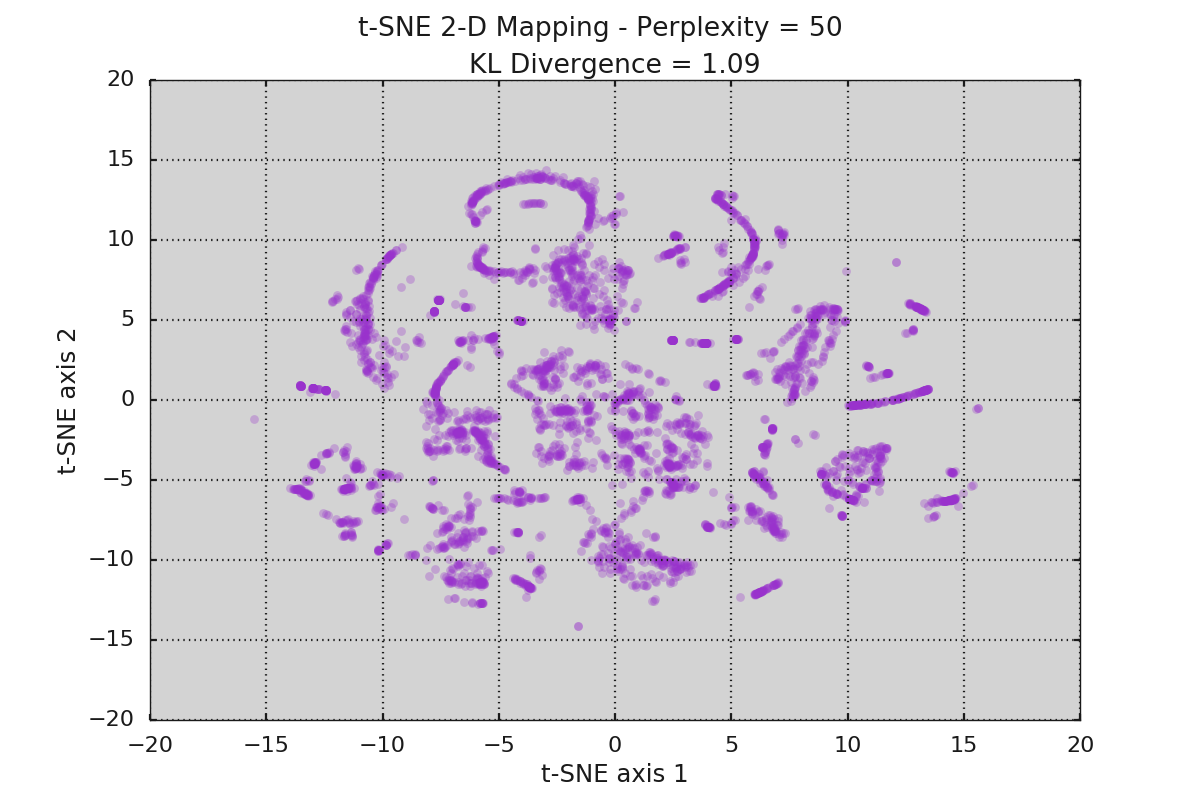
\includegraphics[width=\textwidth, height=\textheight, keepaspectratio]{perplexity.png}
 	\caption{Spread of data visulized using t-sne.}
	\label{figure:perplexity}

\end{figure}
\FloatBarrier
%
\FloatBarrier
\begin{table}
\begin{center}
\caption{Algorithms and evaluation methods}
\label{table:algorithmsandmethods}
\begin{tabular}{p{50mm} p{60mm}}
\hline
\rule{0pt}{12pt}
Algorithm	&	Models	\\[2pt]
\hline
Regression 	&	1.        Multiple Regression	\newline
				2.        Support Vector Machine	??  \newline
				3.        Decision Tree	?? Random Forest\\
Unsupervised Learning	&	1.        Clustering	\newline
				\hspace*{5mm} a.        K-means	\newline
				\hspace*{5mm} b.        Hierarchical 	\newline
				2.         T-Distributed Stochastic Neighbor Embedding
				\\[2pt]
\hline
\end{tabular}
\end{center}
\end{table}
\FloatBarrier
%
\section{Results}
%
\subsection{Data aggregation and grid cell assignment}


The results of several of the data sets aggregated and assigned to each respective grid cell are shown in following figures. In summary, the following features were mapped into the grid cells as candidate features to participate in the modeling :

\FloatBarrier
\begin{table}
\begin{center}
\caption{Feature Definition}
\label{table : featureDefinition}
\begin{tabular}{p{50mm} p{60mm}}
\hline
\rule{0pt}{12pt}
Data category & Specific feature definition	\\[2pt]
\hline
Non-pedestrian accidents 		& Number Events \newline
															Sum cost (NSC) for events \\
Pedestrian survey responses & TBD in next update \\
Reported near misses 				& Number events \newline
                                                            Categorical feature counts \\
Street surface areas 				& Surface total length \newline
                                                            Sum lane counts  \\
Walk Scores 								& Max, Mean, Min  \\
Fire incidents 								& TBD in next update  \\
Non-emergency service requests & Sum number requests \newline
                                                                      Categorical feature counts\\ 
Property values \& uses 			& Median prperty values \newline
                                                            Number of property transfers in 10-year period  \\
Public transportation accessibility & Distance to nearest bus stop \\[2pt]
\hline
\end{tabular}
\end{center}
\end{table}
\FloatBarrier
%

\FloatBarrier
%Figure ~\ref{figure : dataFeatureDevelopment}. \newline
\begin{figure}
  \begin{subfigure}[b]{0.5\textwidth}
    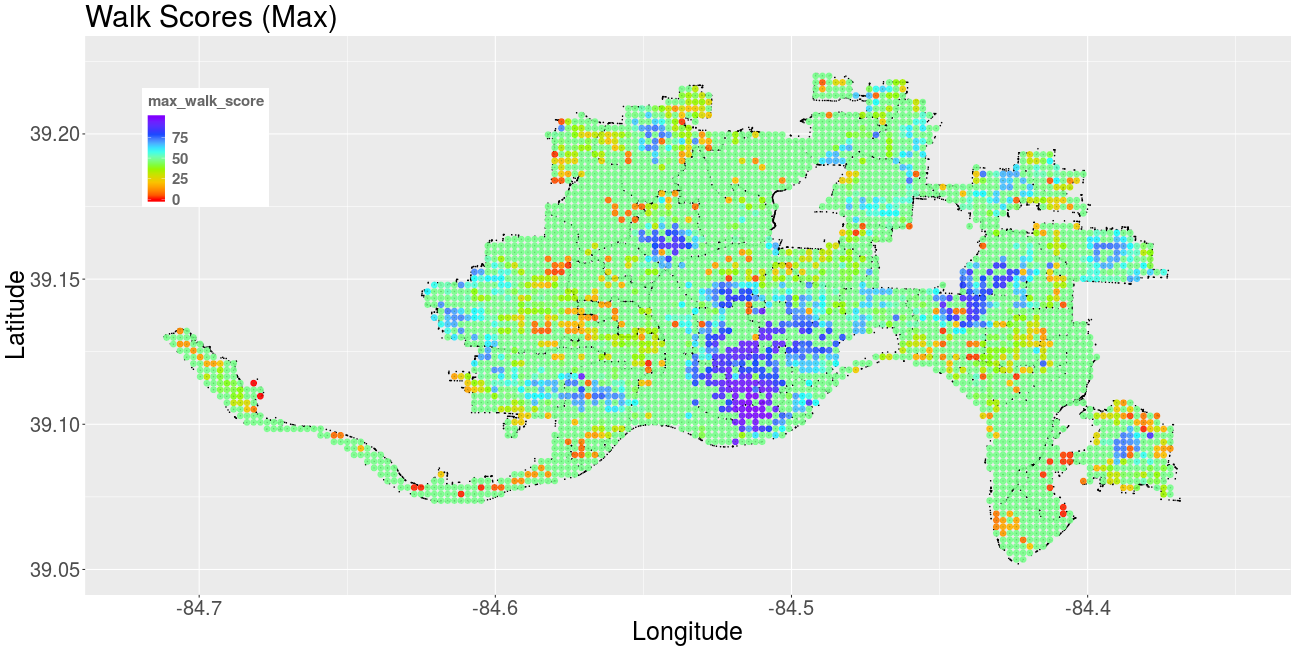
\includegraphics[width = \textwidth, height = \textheight, keepaspectratio]{maxWalkScores.png}
    \caption{Walk Score - Max values}
    \label{figure : 1}
  \end{subfigure}
  %
  \begin{subfigure}[b]{0.5\textwidth}
    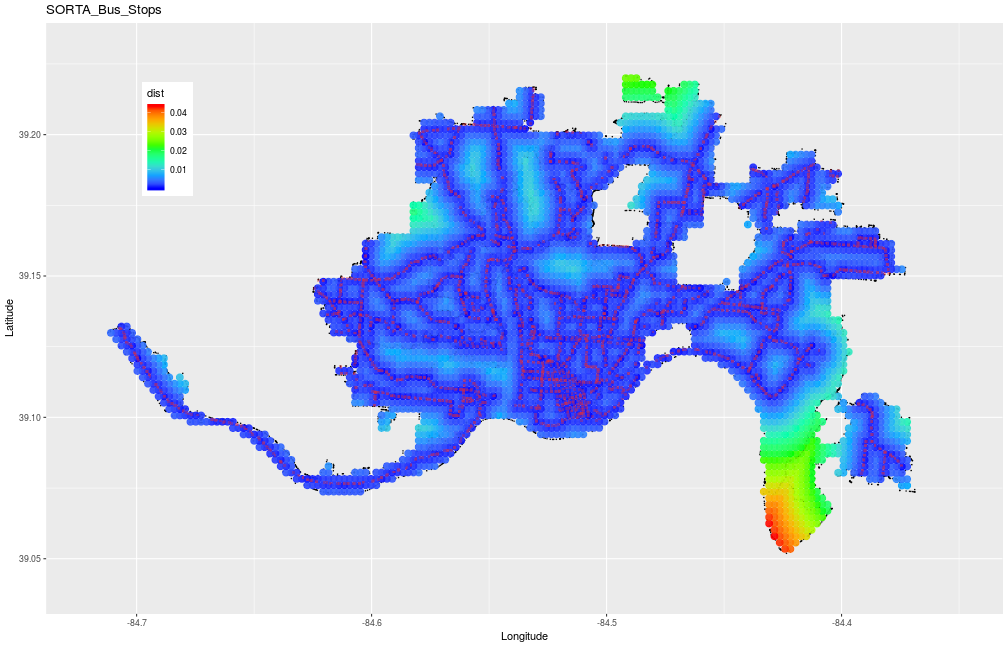
\includegraphics[width = \textwidth, height = \textheight, keepaspectratio]{busStopDistance.png}
    \caption{Public Transportation Accessibility}
    \label{figure : 2}
  \end{subfigure}
\end{figure}
\FloatBarrier

%Figure ~\ref{figure : trafficAccidents}. \newline
\FloatBarrier
\begin{figure}
 	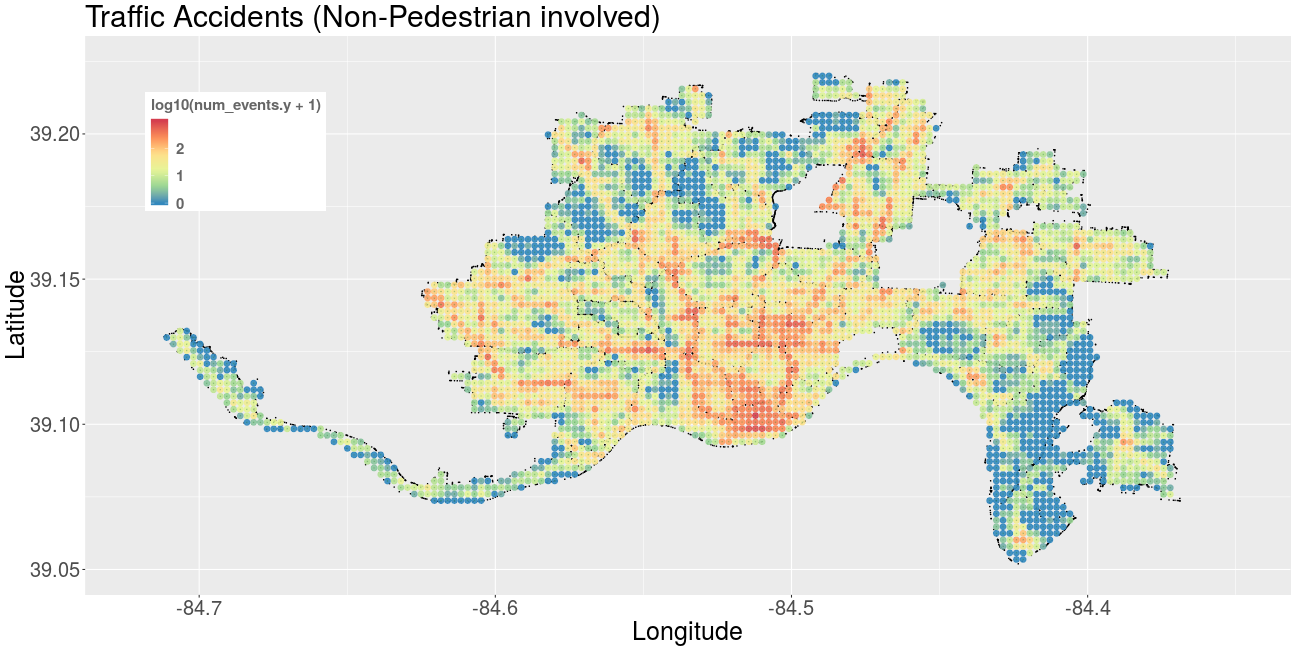
\includegraphics[width=0.5\textwidth, height=0.5\textheight, keepaspectratio]{trafficAccidents.png}
 	\caption{Number of Traffic Accidents (Non-pedestrian involved)}
	\label{figure : trafficAccidents}
\end{figure}
\FloatBarrier

\subsection{Random Forest - Binary Model}

The random forest model which we deployed to estimate occurrence of pedestrian related events produces the result of 75\% true positive, 20\% false positive with a detection threshold set at 0.20. This result provides a balanced compromise between true positive and false positive, as depicted in the following Figure ~\ref{figure : rfroccurve}. \newline
\FloatBarrier
\begin{figure}
 	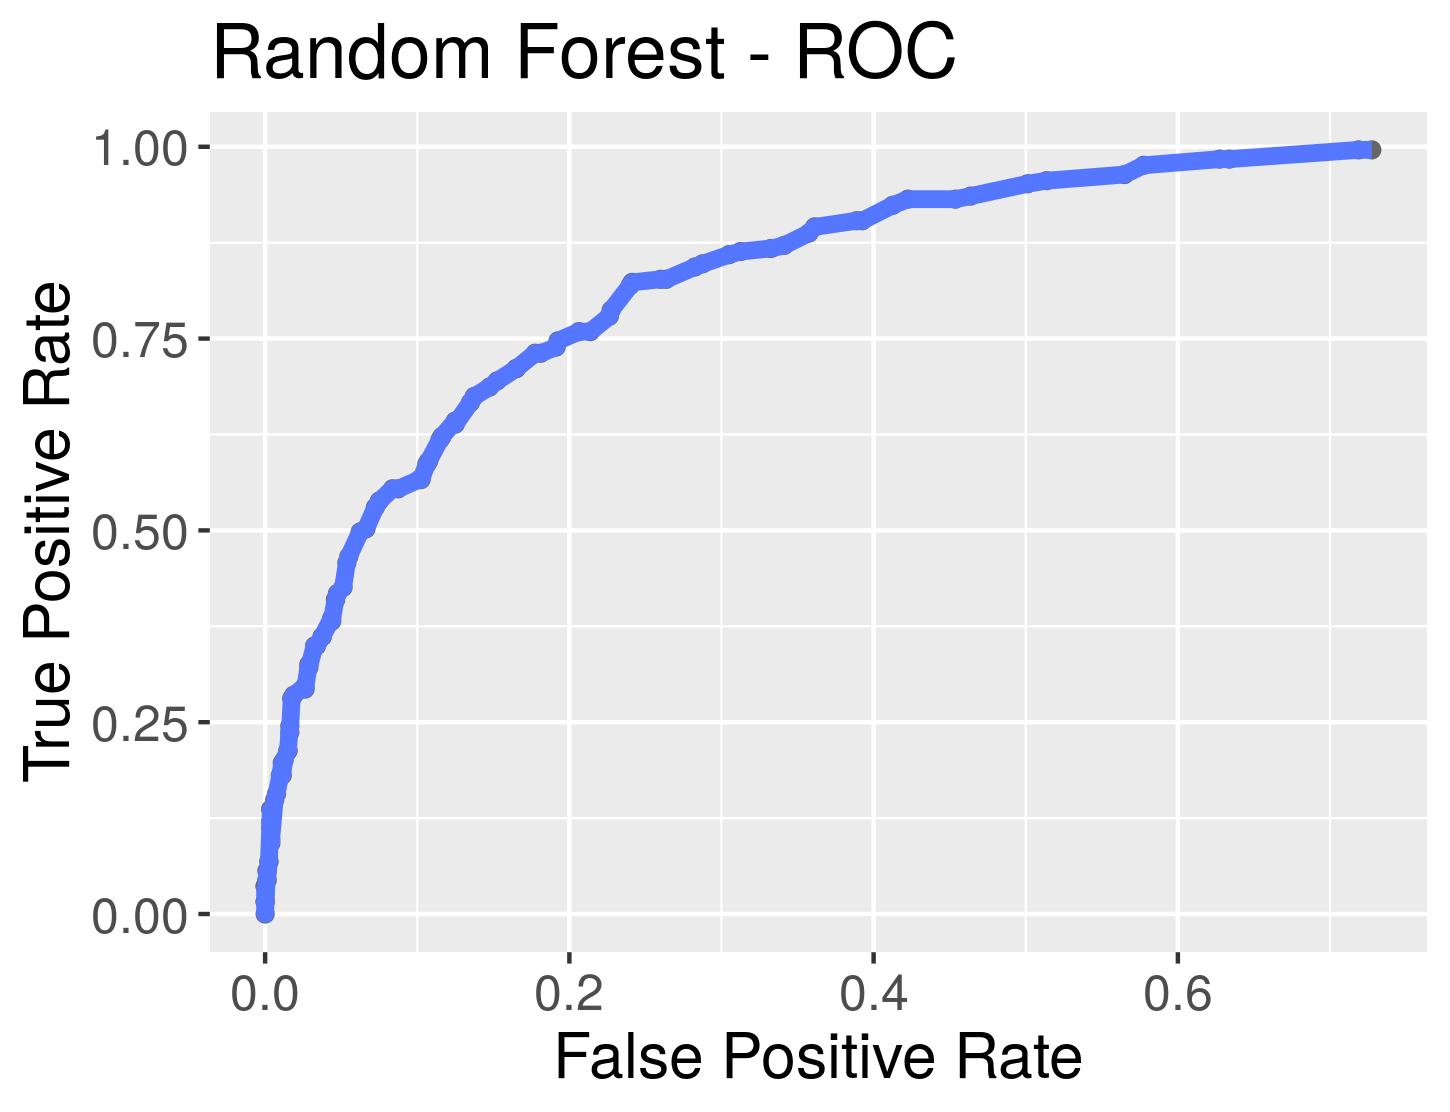
\includegraphics[width=\textwidth, height=\textheight, keepaspectratio]{RFROC.png}
 	\caption{Random forest - binary model - ROC curve}
	\label{figure : rfroccurve}
\end{figure}
\FloatBarrier

As visualized on the map of the city, Figure ~\ref{figure : rfbinarymap}, we observe that (a) the regions of true positve (green) and true negative (light grey) comprise the large majority of the surface area, generally represented by contiguous areas, and confirm the high overall accuracy of the model, (b) that the false positive (darker grey) and false negative (red dots) are consistently along the border regions between otherwise true positive or true negative regions, and (c)  the false negative regions are distinct non-connected grid cells at somewhat widely distributed locations around the city.
\newline

\FloatBarrier
\begin{figure}
 	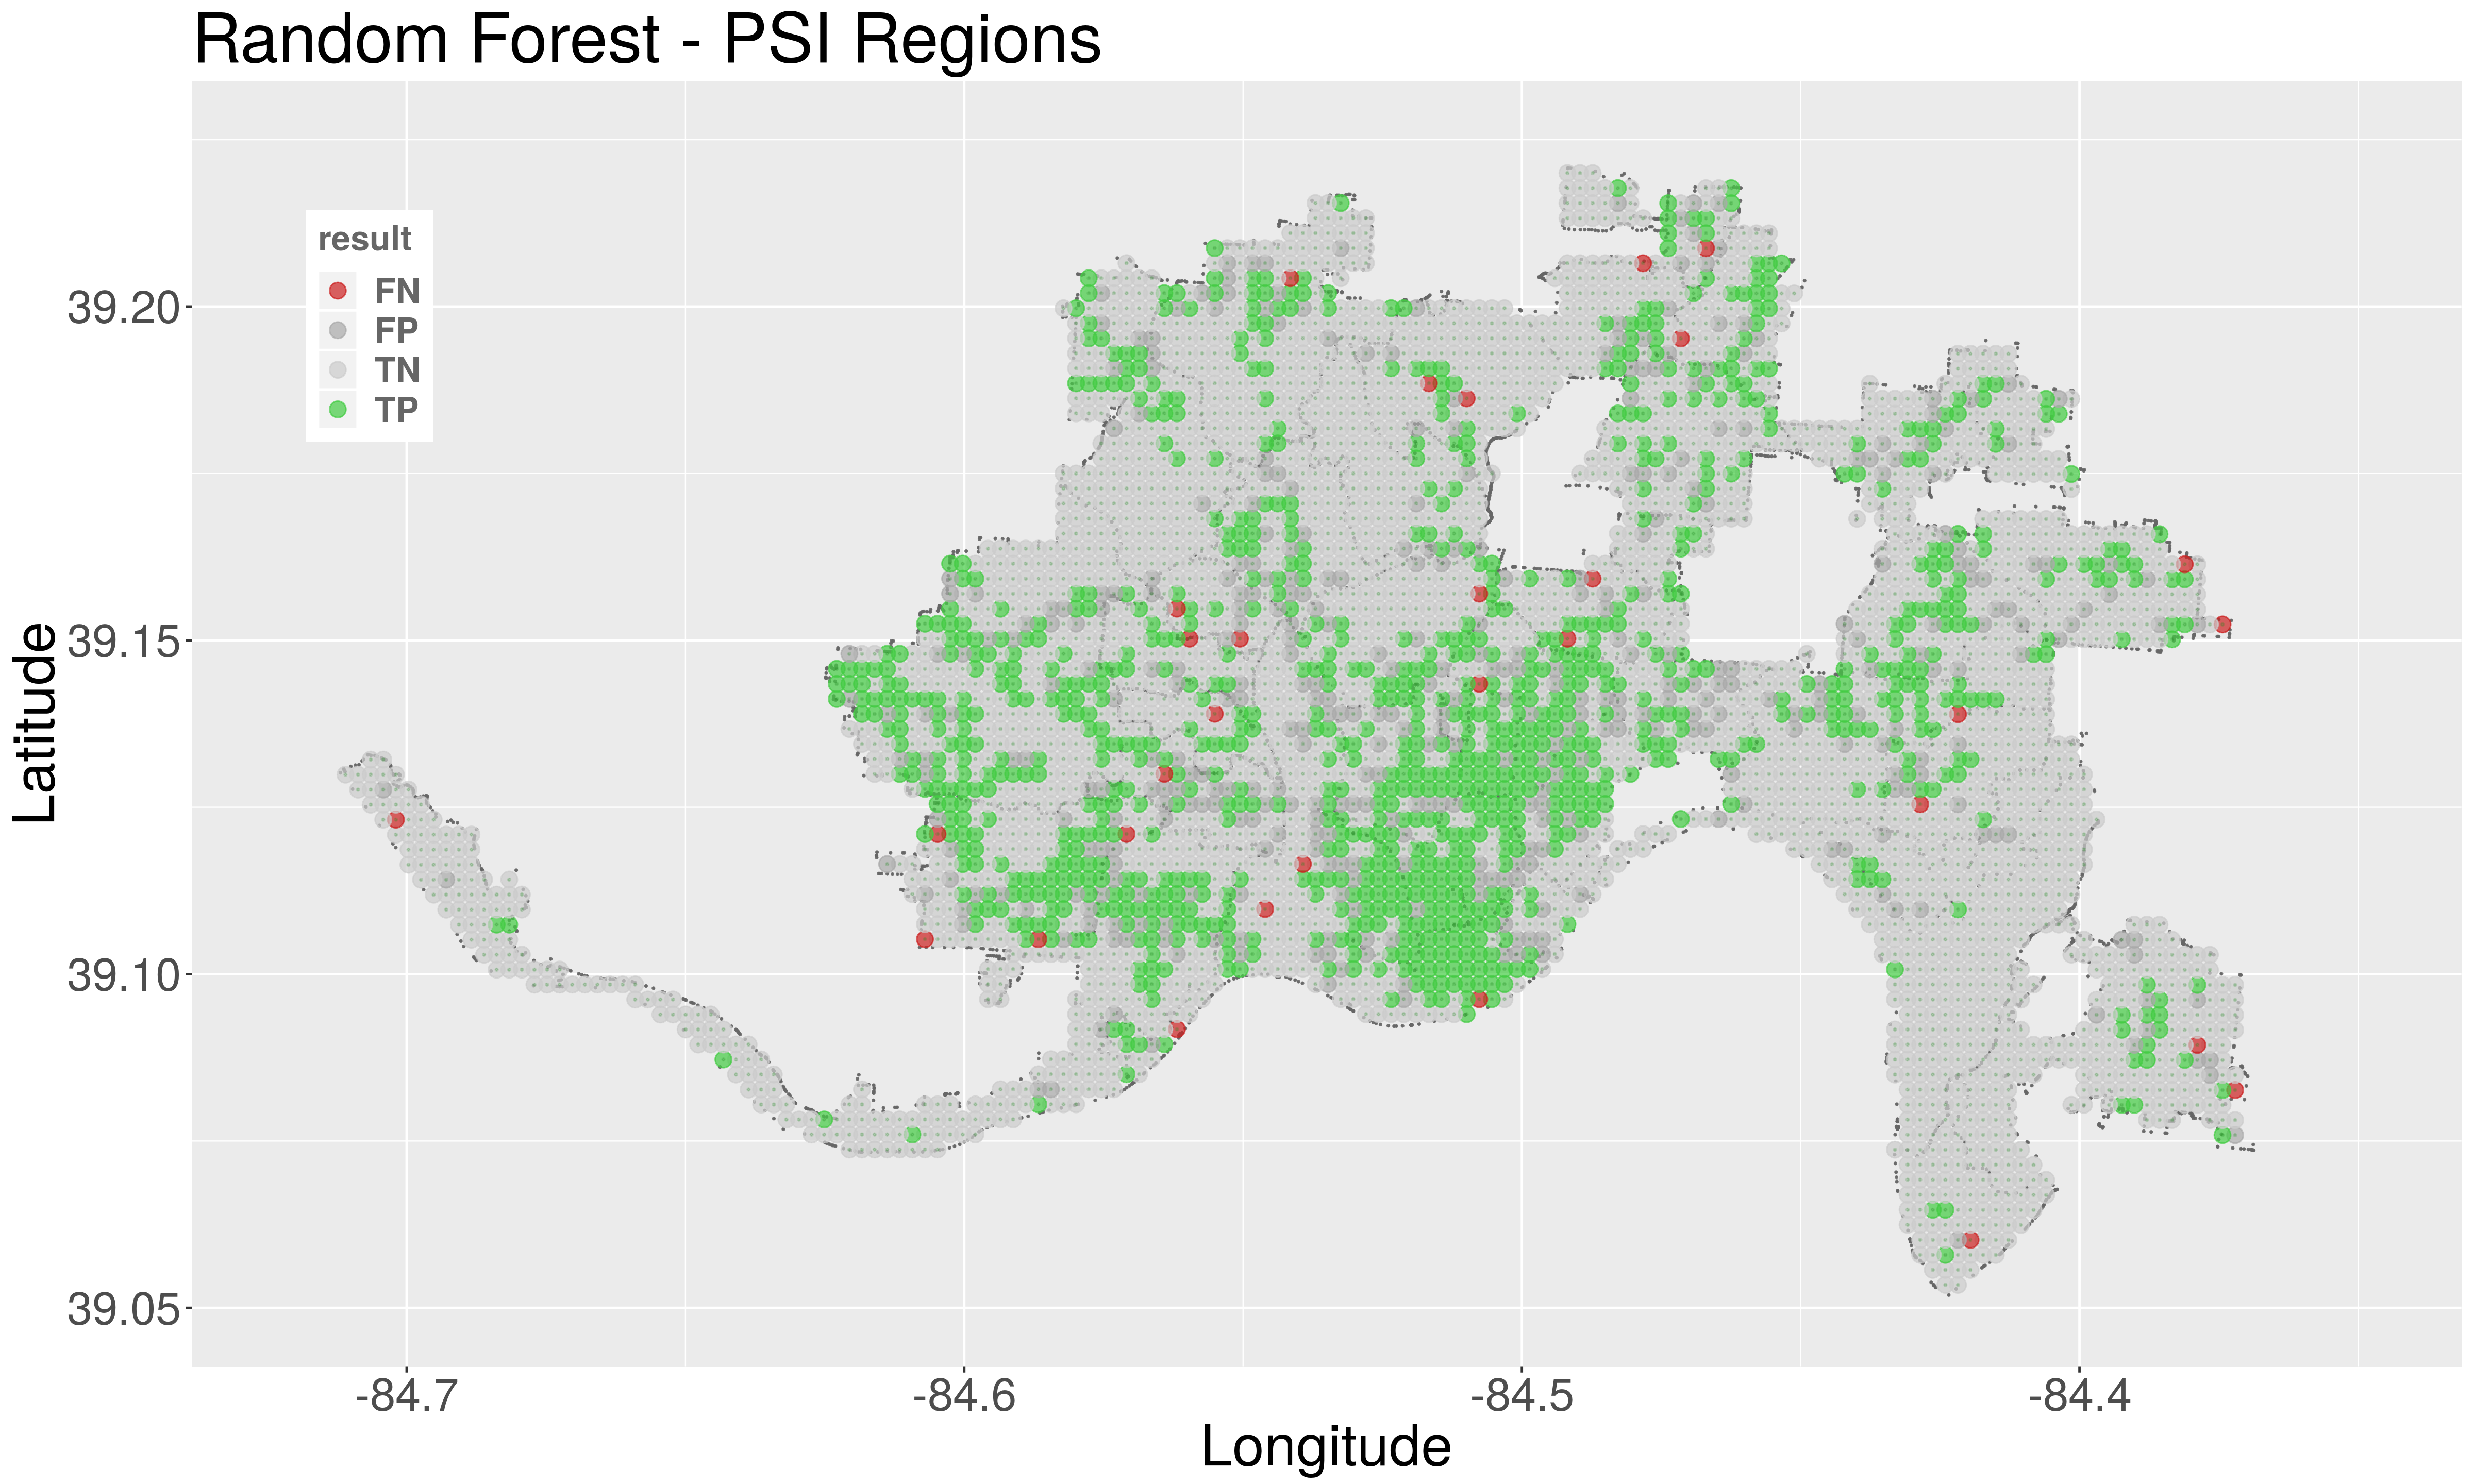
\includegraphics[width=\textwidth, height=\textheight, keepaspectratio]{RFBinaryResultsMap.png}
 	\caption{Distribution of random forest model results visualized on city map}
	\label{figure : rfbinarymap}
\end{figure}
\FloatBarrier

\subsection{Multi-variate linear regression - Cost Model}

\FloatBarrier
\begin{table}[!h]
\begin{center}
\caption{Analysis of reduced model regression variables.}
\label{table:RegressionAnalysis}
\begin{tabular}{lrrrr}
%{ p{.30\textwidth} p{.20\textwidth} p{.20\textwidth} p{.10\textwidth} p{.15\textwidth}}
\hline
\rule{0pt}{12pt}
Variable
& Estimate (\$)
& Std. Error (\$)
& t-value
& p-value\\[2pt]
\hline
Intercept&310,397&90,519&3.429&0.00064\\
Sum Cost of Damage to People in Non-Pedestrian Accidents&267&31.8&8.391&$<$ 2e-16\\
Unsanitary Food Operations&39,796&8,189&4.86&1.40E-06\\
Intercept&310,397&90,519&3.429&0.00064\\
Maximum Walk Score&5,638&1758&3.207&0.00139\\
Water Leaks and Breaks&-72,140&24,776&-2.912&0.00369\\
Crosswalk Needed&117,618&45,848&2.565&0.01048\\
Number of Police Properties&14,442&5,850&2.469&0.01377\\
Vehicles Running Red Lights / Stop Signs&50,332&24,291&2.072&0.03856\\
Unkempt Flora&3,998&2,158&1.853&0.06429\\
Speeding&-62,700&34,132&-1.837&0.06658\\
Parking Close to Intersection&-146,340&82,879&-1.766&0.07781\\
Parking on Sidewalk&257,246&147,334&1.746&0.08117\\[2pt]
\hline
\end{tabular}
\end{center}
\end{table}
\FloatBarrier

Table ~\ref{table:RegressionAnalysis} shows the explanatory variables for the reduced multiple linear regression model. This model had an R2 value of .2021 and an adjusted R2 value of .1917. 

\FloatBarrier
\begin{figure}
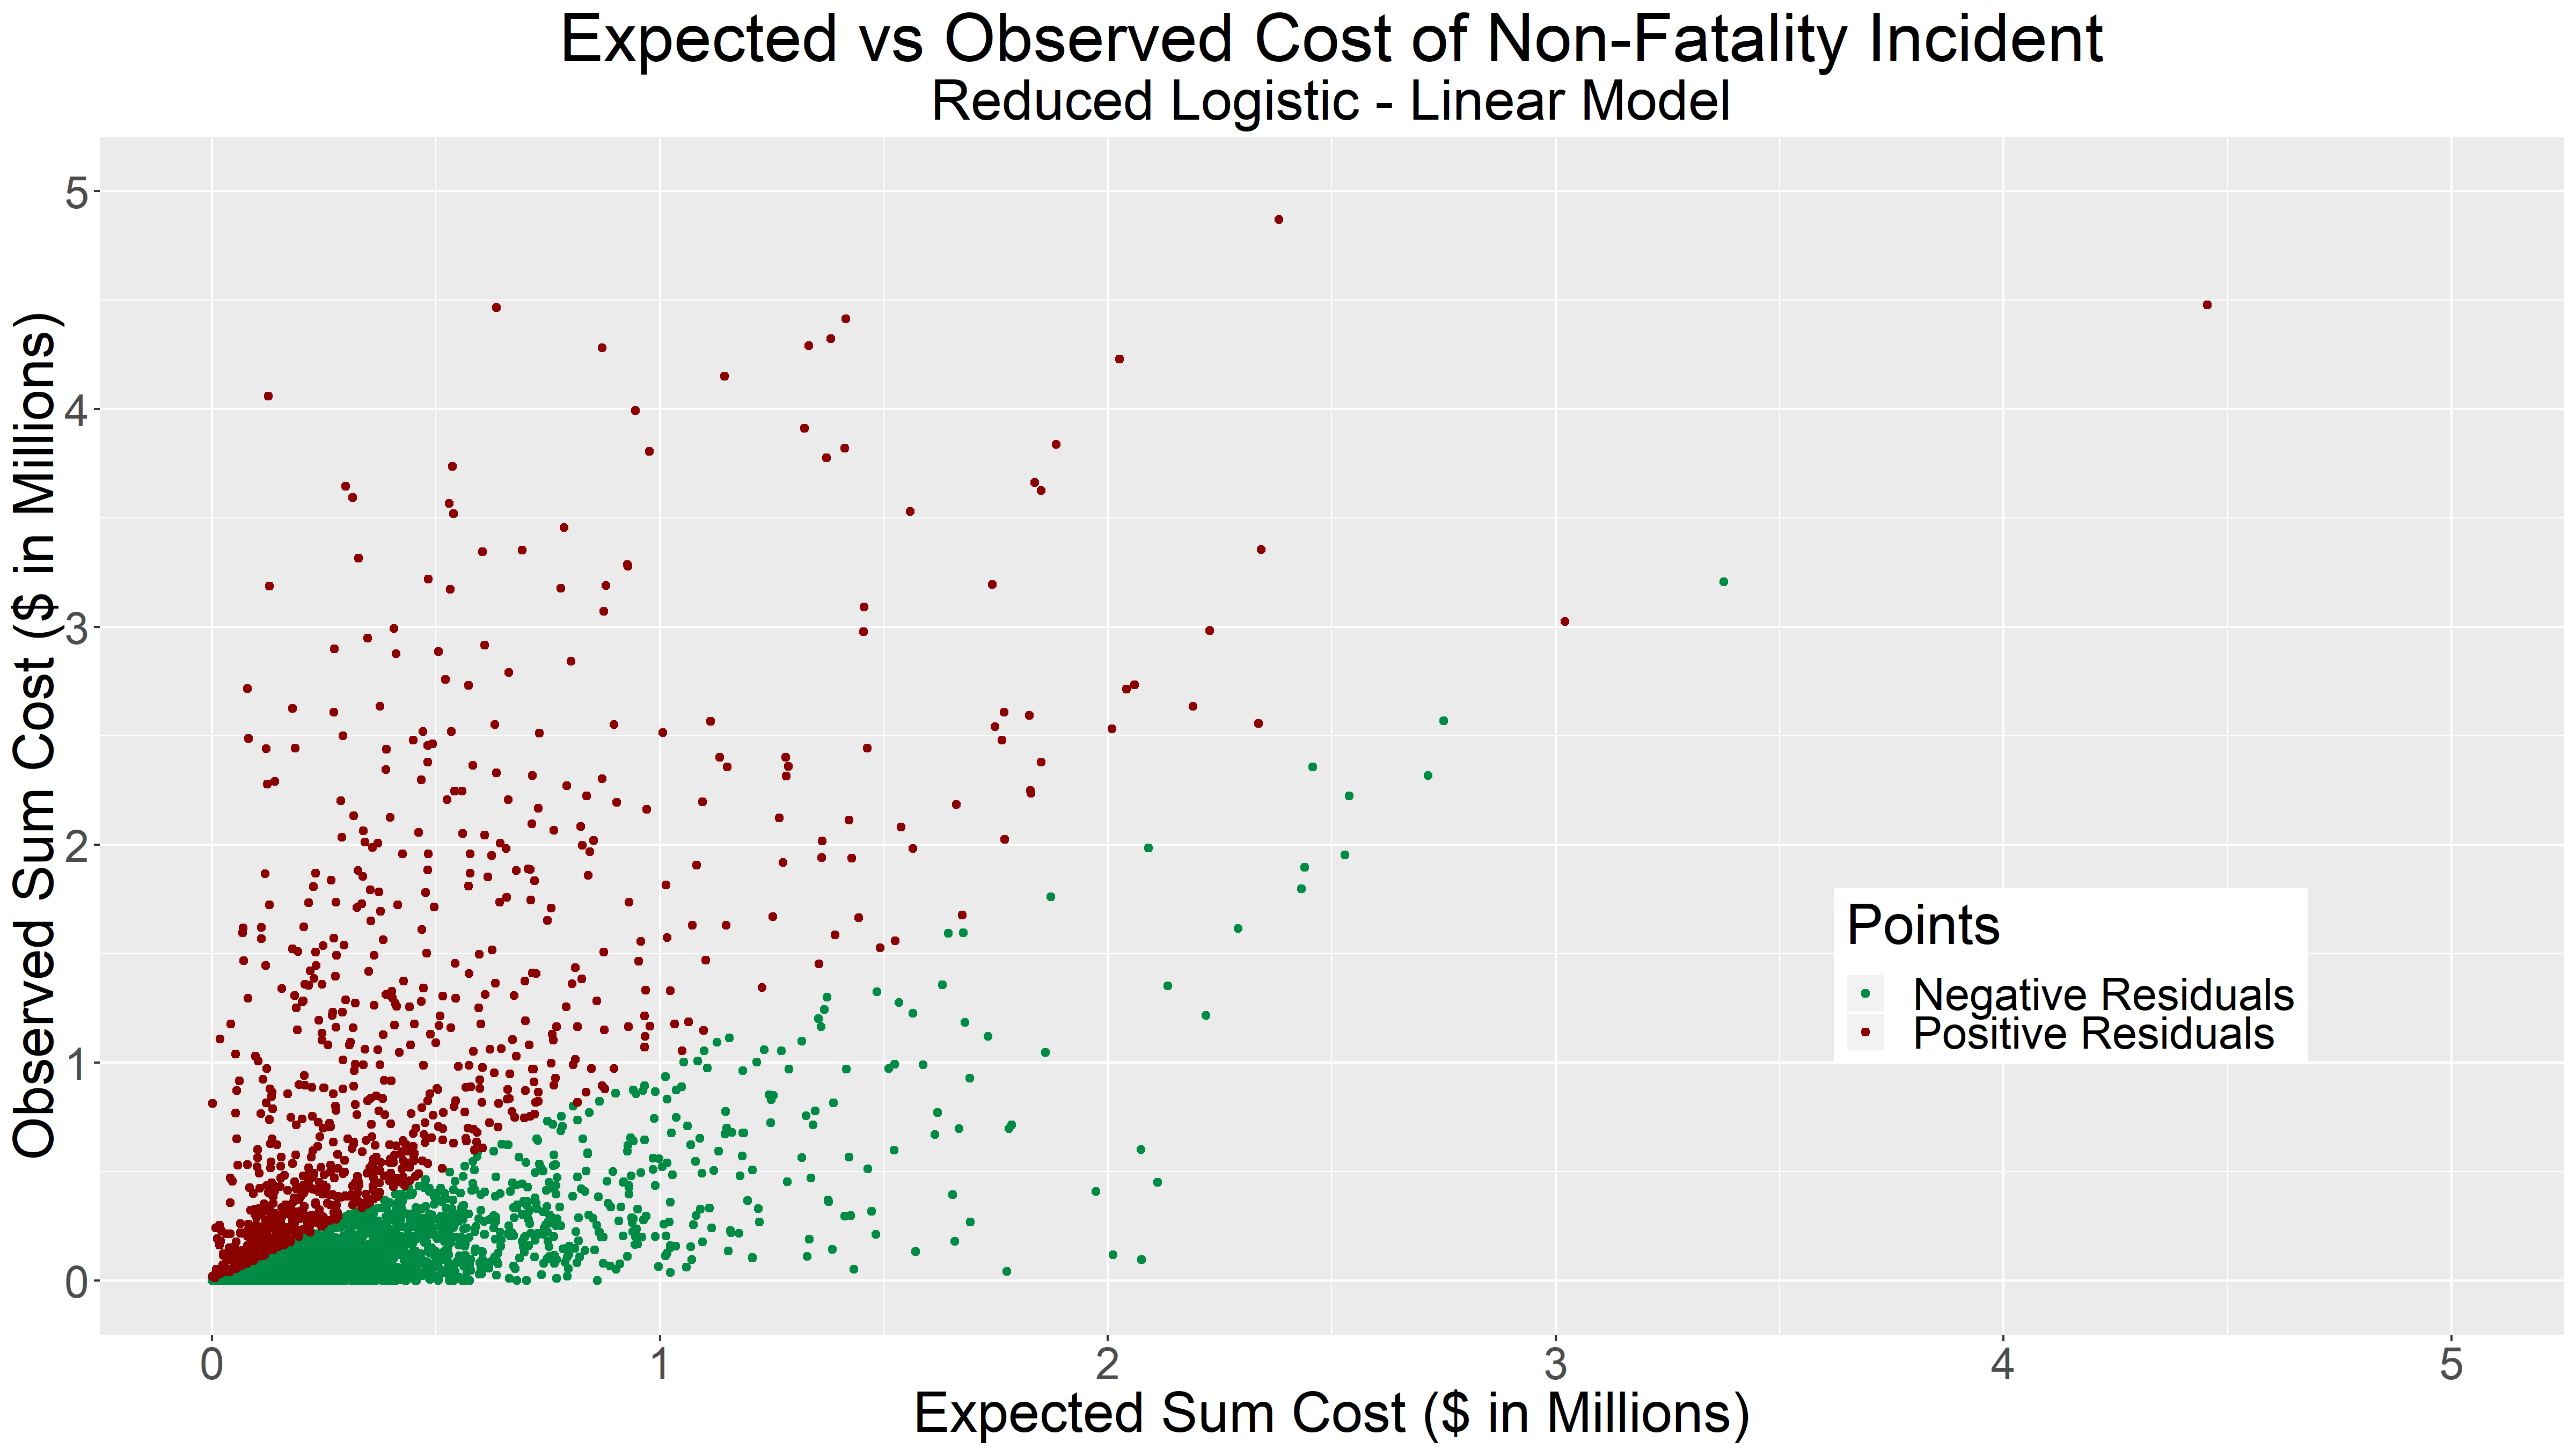
\includegraphics[width=\textwidth, height=\textheight, keepaspectratio]{000LinearModelReduced.png}
\caption{Comparison of expected and observed non-fatality pedestrian incident costs.}
\label{figure:LinearModelReduced}

\end{figure}
\FloatBarrier

Figure ~\ref{figure:LinearModelReduced} is a comparison between the observed and actual cost of a non-fatality incident in Cincinnati.

\FloatBarrier
\begin{figure}
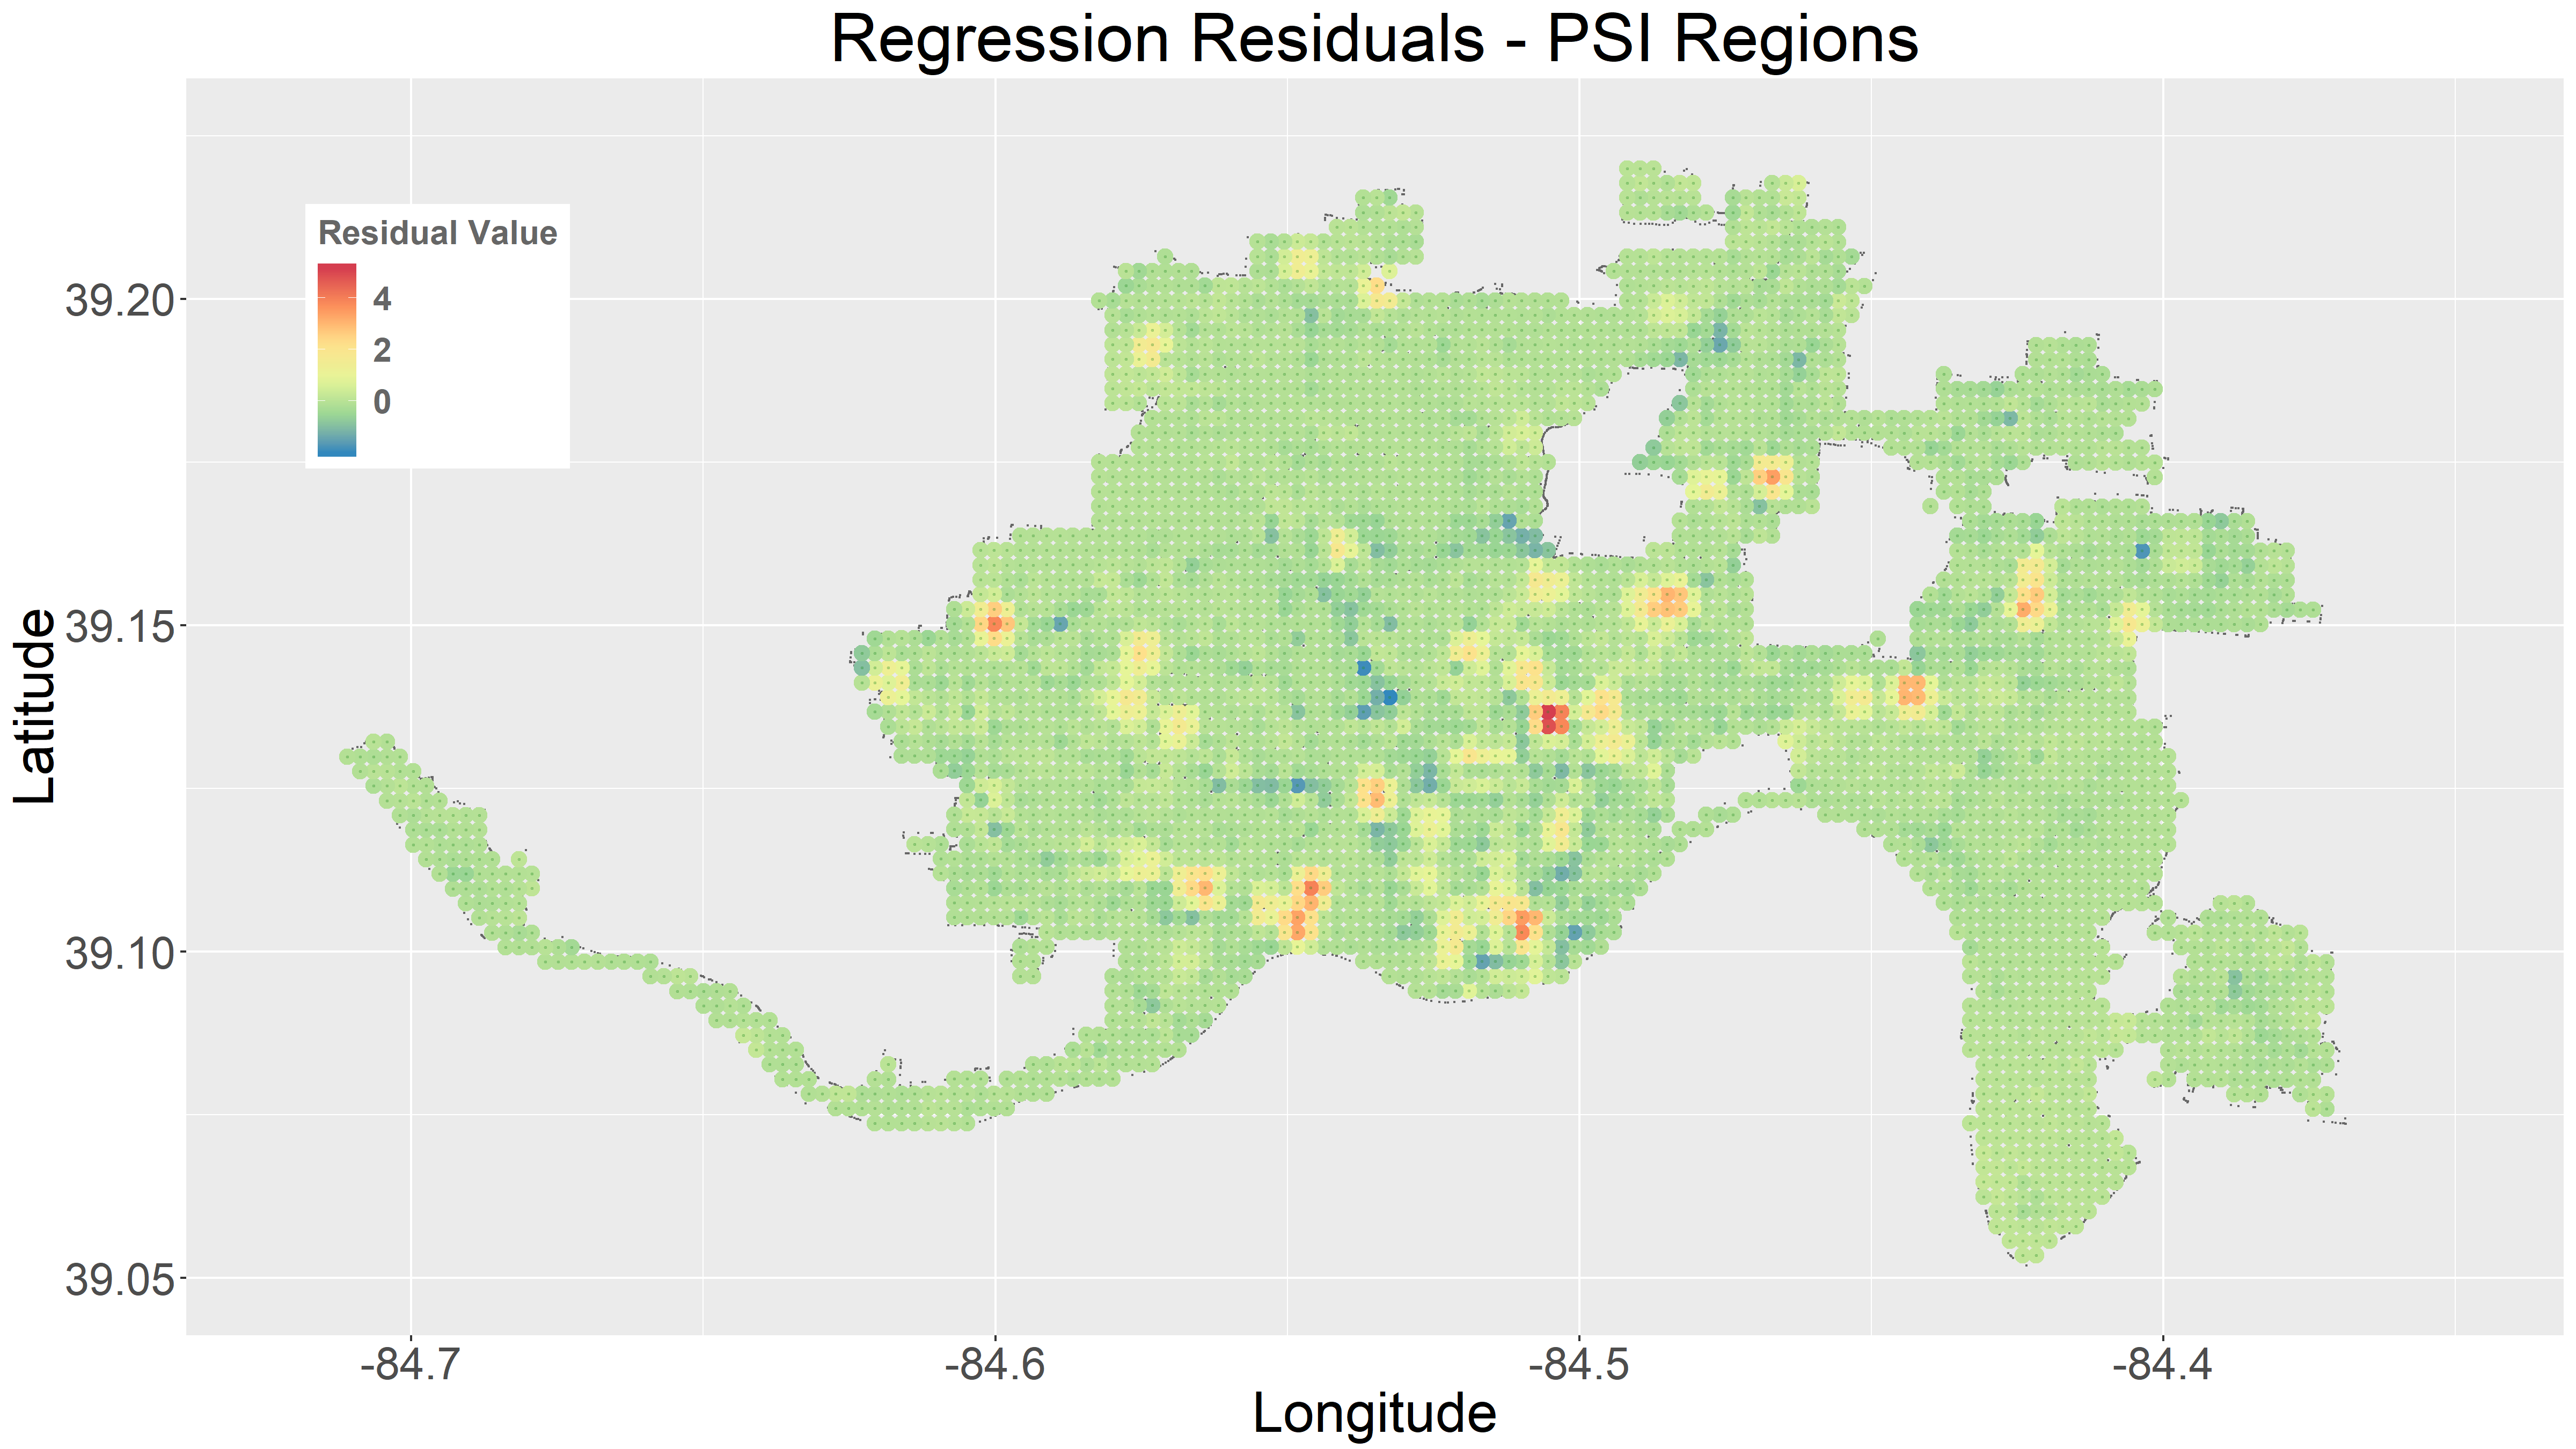
\includegraphics[width=\textwidth, height=\textheight, keepaspectratio]{000ResidualsPlot.png}
\caption{A map of Cincinnati identifying areas with PSI in the darkest red.}
\label{figure:ResidualsPlot}

\end{figure}
\FloatBarrier

Figure ~\ref{figure:ResidualsPlot} shows the residuals mapped back to the map of Cincinnati.

\subsection{Unsupervised learning - Neighborhood characterization}

For each attribute, distribution and scatter plots are generated to visualize the impact of it in the cluster. Attributes like property type commercial was heavily clustered in 1 or the green areas as in Figure ~\ref{figure:kmeansongrid}, while residential and industrial were lot more distributed. Issues like metal trash were more in industrial areas which was in the cluster 2 or red neighborhoods. Water leak was more an issue in cluster 0 or blue areas.

Combining attribute behavior and clusters on the map, pedestrian saftey issues in each cluster are identified. These issues are then mapped to the actual locality or neighborhood to draw conclusions.

\FloatBarrier
\begin{figure}
 	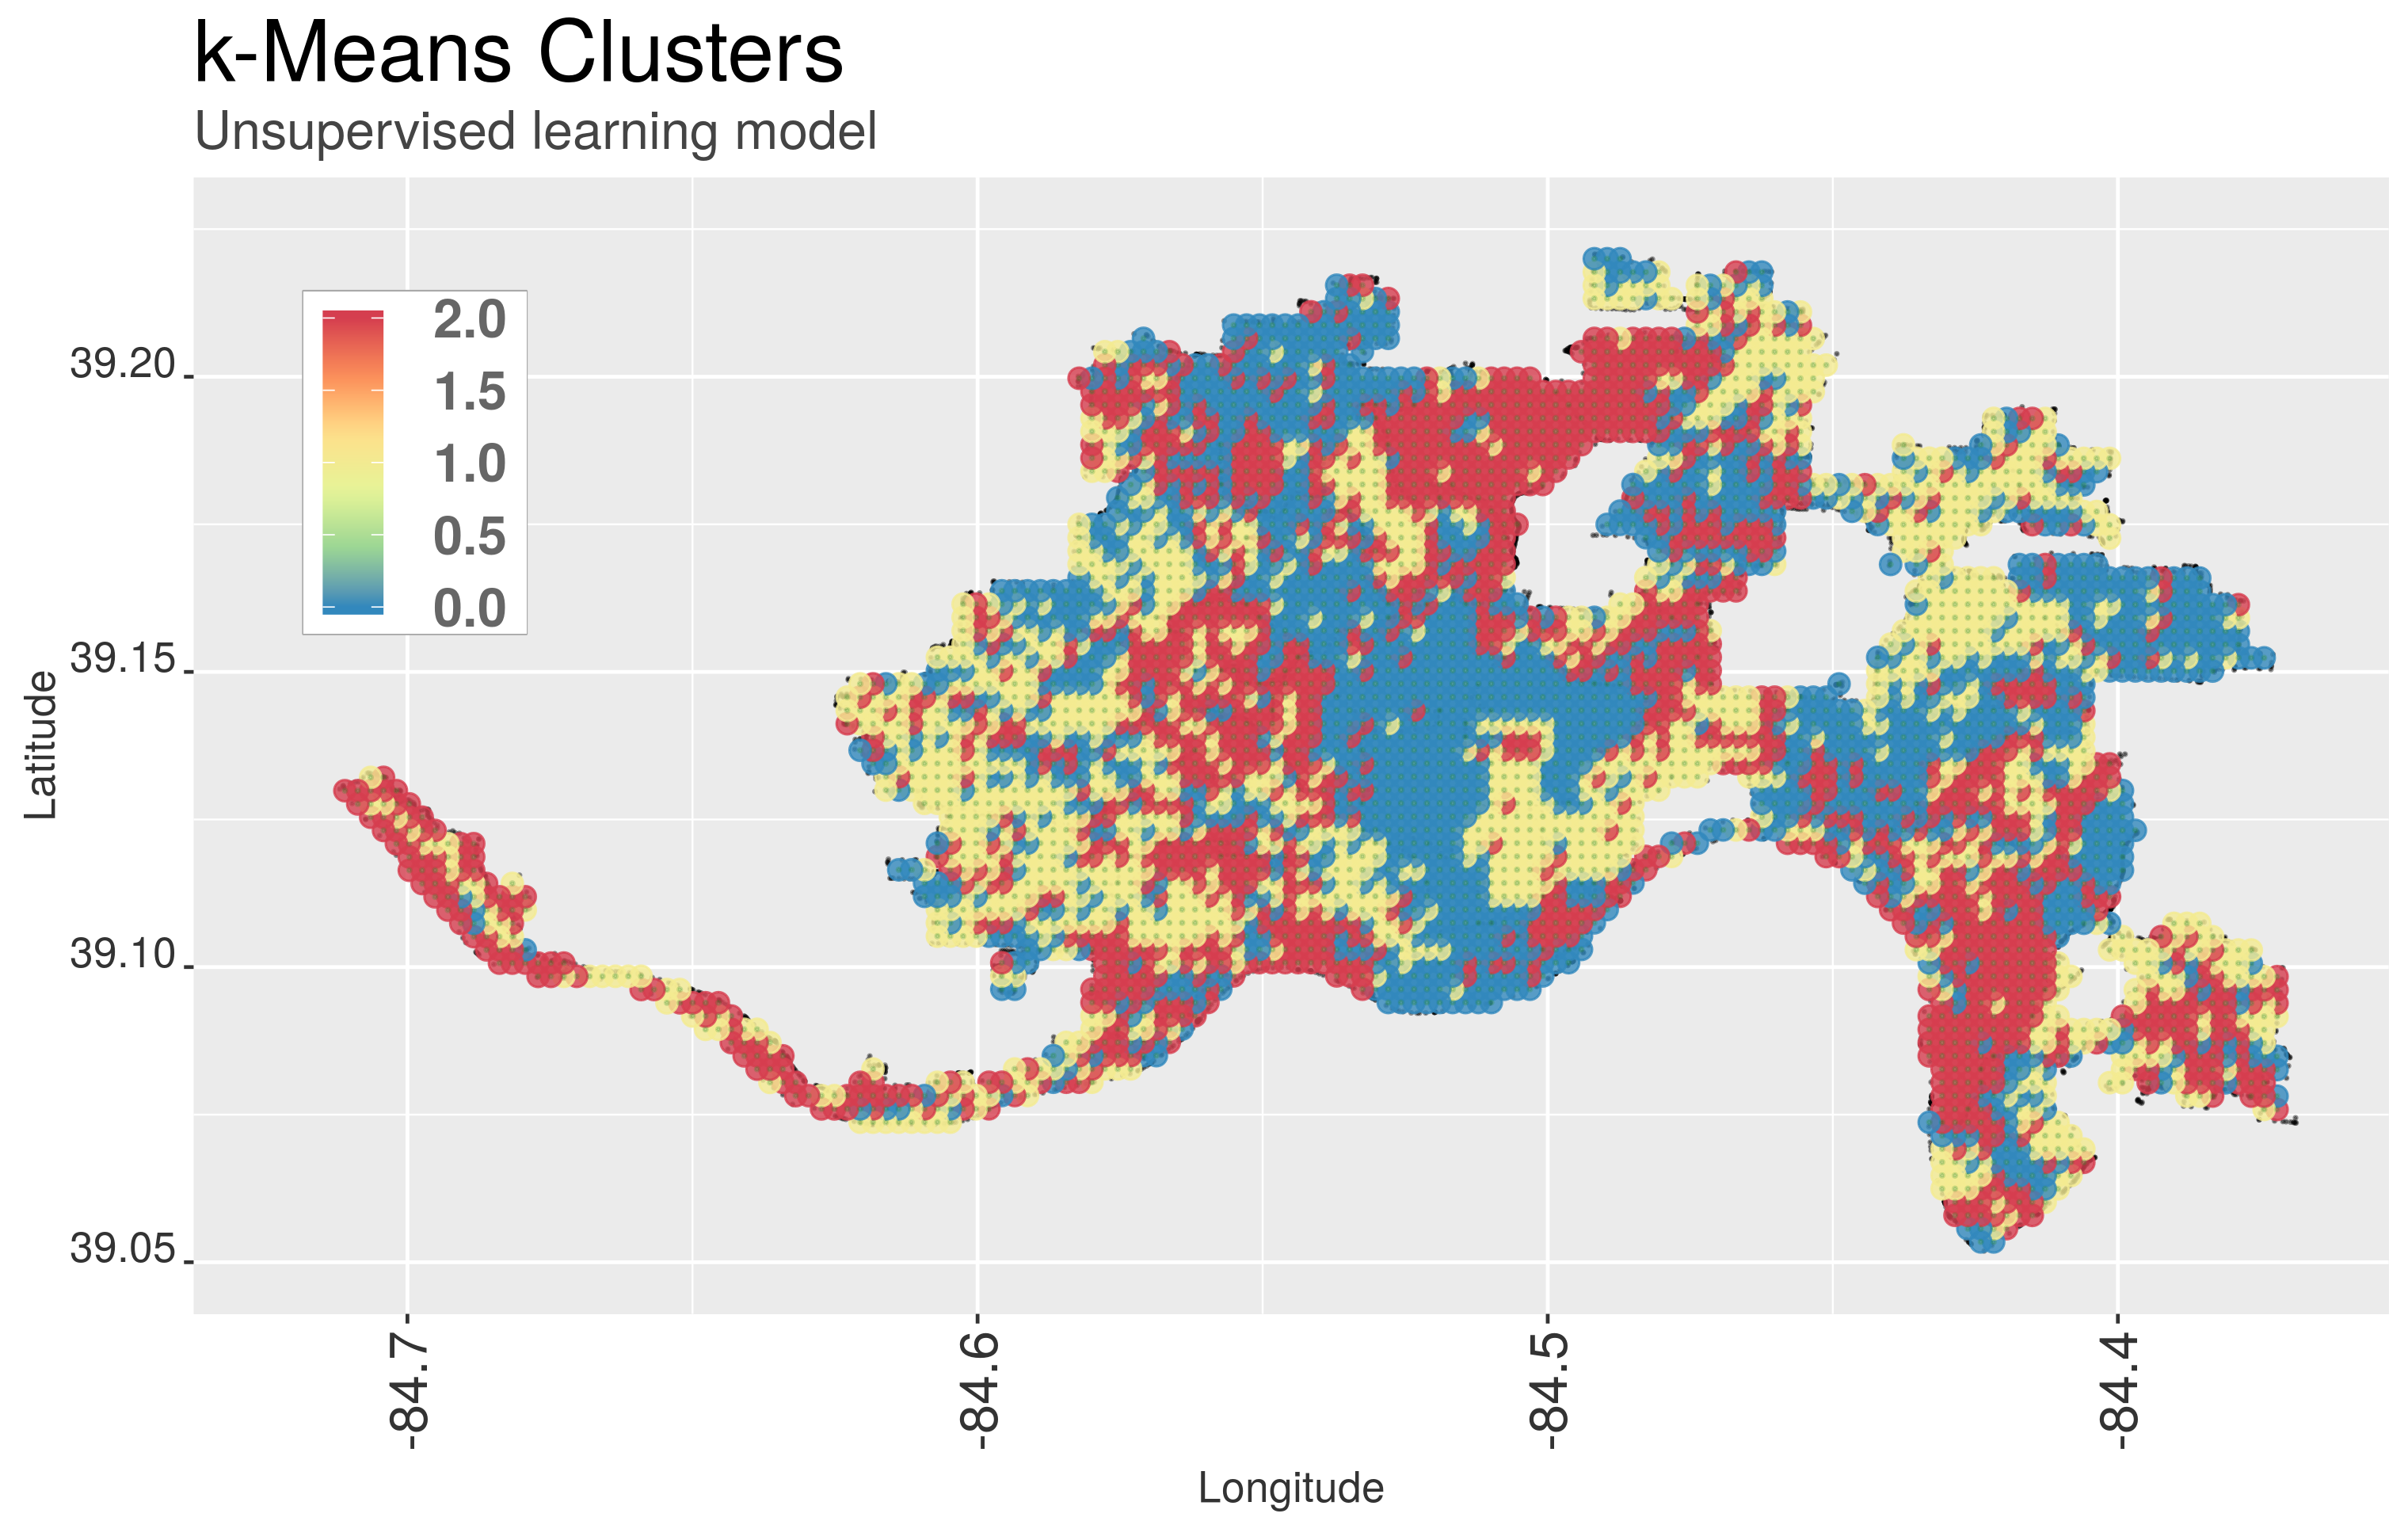
\includegraphics[width=\textwidth, height=\textheight, keepaspectratio]{kmeansongrid.png}
 	\caption{Cluster results on map of Cincinatti}
	\label{figure:kmeansongrid}
\end{figure}
\FloatBarrier


Initial results from part 1 of our methodology have produced graphs as shown in Figure ~\ref{figure:SumCrashPlot}. \newline
\FloatBarrier
\begin{figure}
 	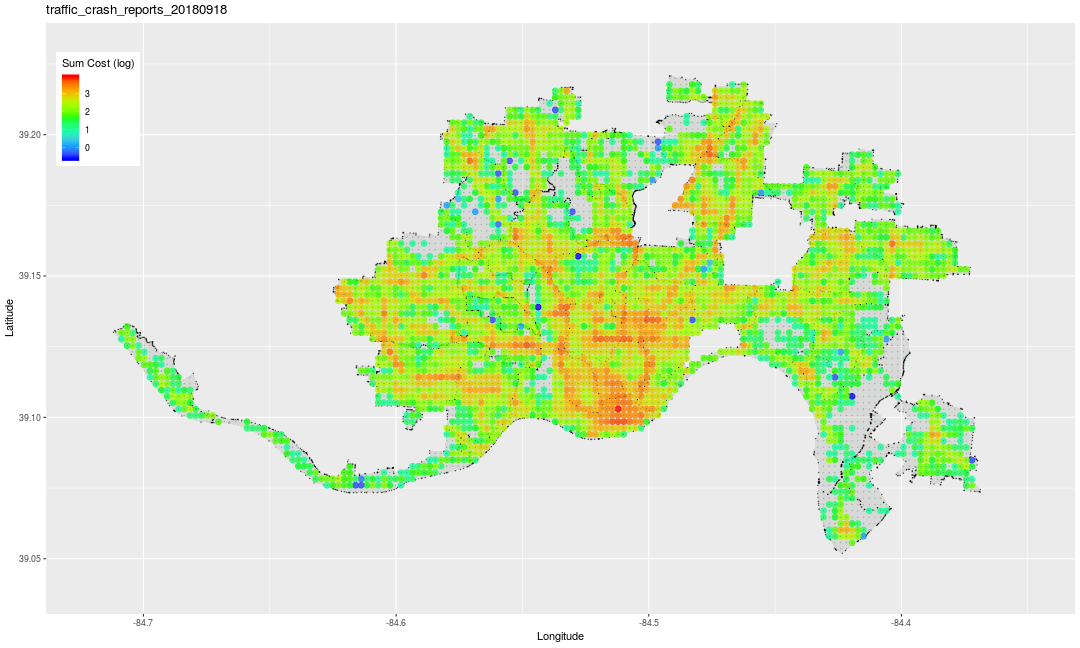
\includegraphics[width=\textwidth, height=\textheight, keepaspectratio]{TrafficCrashReports20180918SumCostMapped2Grid.png}
 	\caption{Sum cost of traffic crashes reported from 2012 to October 2018 involving pedestrians by grid cells.}
	\label{figure:SumCrashPlot}
\end{figure}
\FloatBarrier
%
\section{Analysis}
%
\subsection{Random Forest - Binary Model}

The focus of this effort is to identify locations within the city that indicate highest potential for safety improvement. Consistent with the concept as defined and implemented in other works, the model incidents for which the observed experience exceeds the expected (model output) response are the regions with potential for safety improvement. In the context of a binary model, as was completed here with the random forest model, the regions of PSI are the false negative points on the grid map, as presented in Figure ~\ref{figure : rfbinarymap}. For these grid cells, the model result was no expected pedestrian events, yet the observed experience exceeded this expected response. In this case, there are 31 grid cells identified with potential for safety improvement. In the next update to this draft, we will present what are the unique characteristics of these grid cells, where they are located geographically within the city (street and intersection identification) and what was the ac
%

\subsection{Multi-Variate Regression - Cost Model}
The results from the prior section provide a numerical and visual way to interpret the model. Because the regression model was subset based on the total cost of damage to the pedestrian excluding events resulting in \$5 million or more in damages, this results in the scope of the model being limited to non-fatality incidents. The regression model is able to explain 20\% of the variance in the cost of a non-fatality incident. This model consists of many significant variables, such as reports of crosswalks needed and reports of vehicles not obeying traffic signs, and some suggestively significant variables which make sense practically, but do not meet the p-value threshold of .05 such as speeding (p-value = .066), parking close to an intersection (p-value = .077), and parking on the sidewalk (p-value = .081). Most variables present within the model are reports to the non-emergency police telephone number, or the city’s online safety survey. For each incident of report within the grid-cell, the predicted total cost of non-fatality incident changes by the estimated amount. Other non-report variables include the number of police properties present within the grid-cell, the maximum Walk Score value of properties within the grid-cell, and the total cost of damage to people involved in non-pedestrian related (motor vehicle) accidents. 

Figure ~\ref{figure:LinearModelReduced} illustrates the model’s predictive capability as compared to the cost of incident in reality. Points which are colored in red have positive residuals, meaning the model has underestimated the cost. Green points have negative residuals, which mean the model has overestimated the cost. The further away a point is, the larger its absolute residual value is. These distances are displayed on Figure ~\ref{figure:ResidualsPlot}, where the red colored areas correspond to the distant red points. These areas within the city in which the model has underestimated the cost the most have the most potential for safety improvement, because all other factors being equal, there is something about that area which is causing a higher amount of damage to pedestrians.

\subsection{Unsupervised Learning - Neighborhood Characterization}
For each attribute, distribution and scatter plots are generated to visualize the impact of it within the cluster. Attributes like property type: commercial were heavily clustered in 1, or the green areas as in Figure ~\ref{figure:kmeansongrid}, while residential and industrial were lot more distributed. Issues like metal trash were more in industrial areas which was in the cluster 2 or red neighborhoods. Water leak was more an issue in cluster 0 or blue areas.

Combining attribute behavior and clusters on the map, pedestrian saftey issues in each cluster are identified. These issues are then mapped to the actual locality or neighborhood to draw conclusions.

\FloatBarrier
\begin{figure}
 	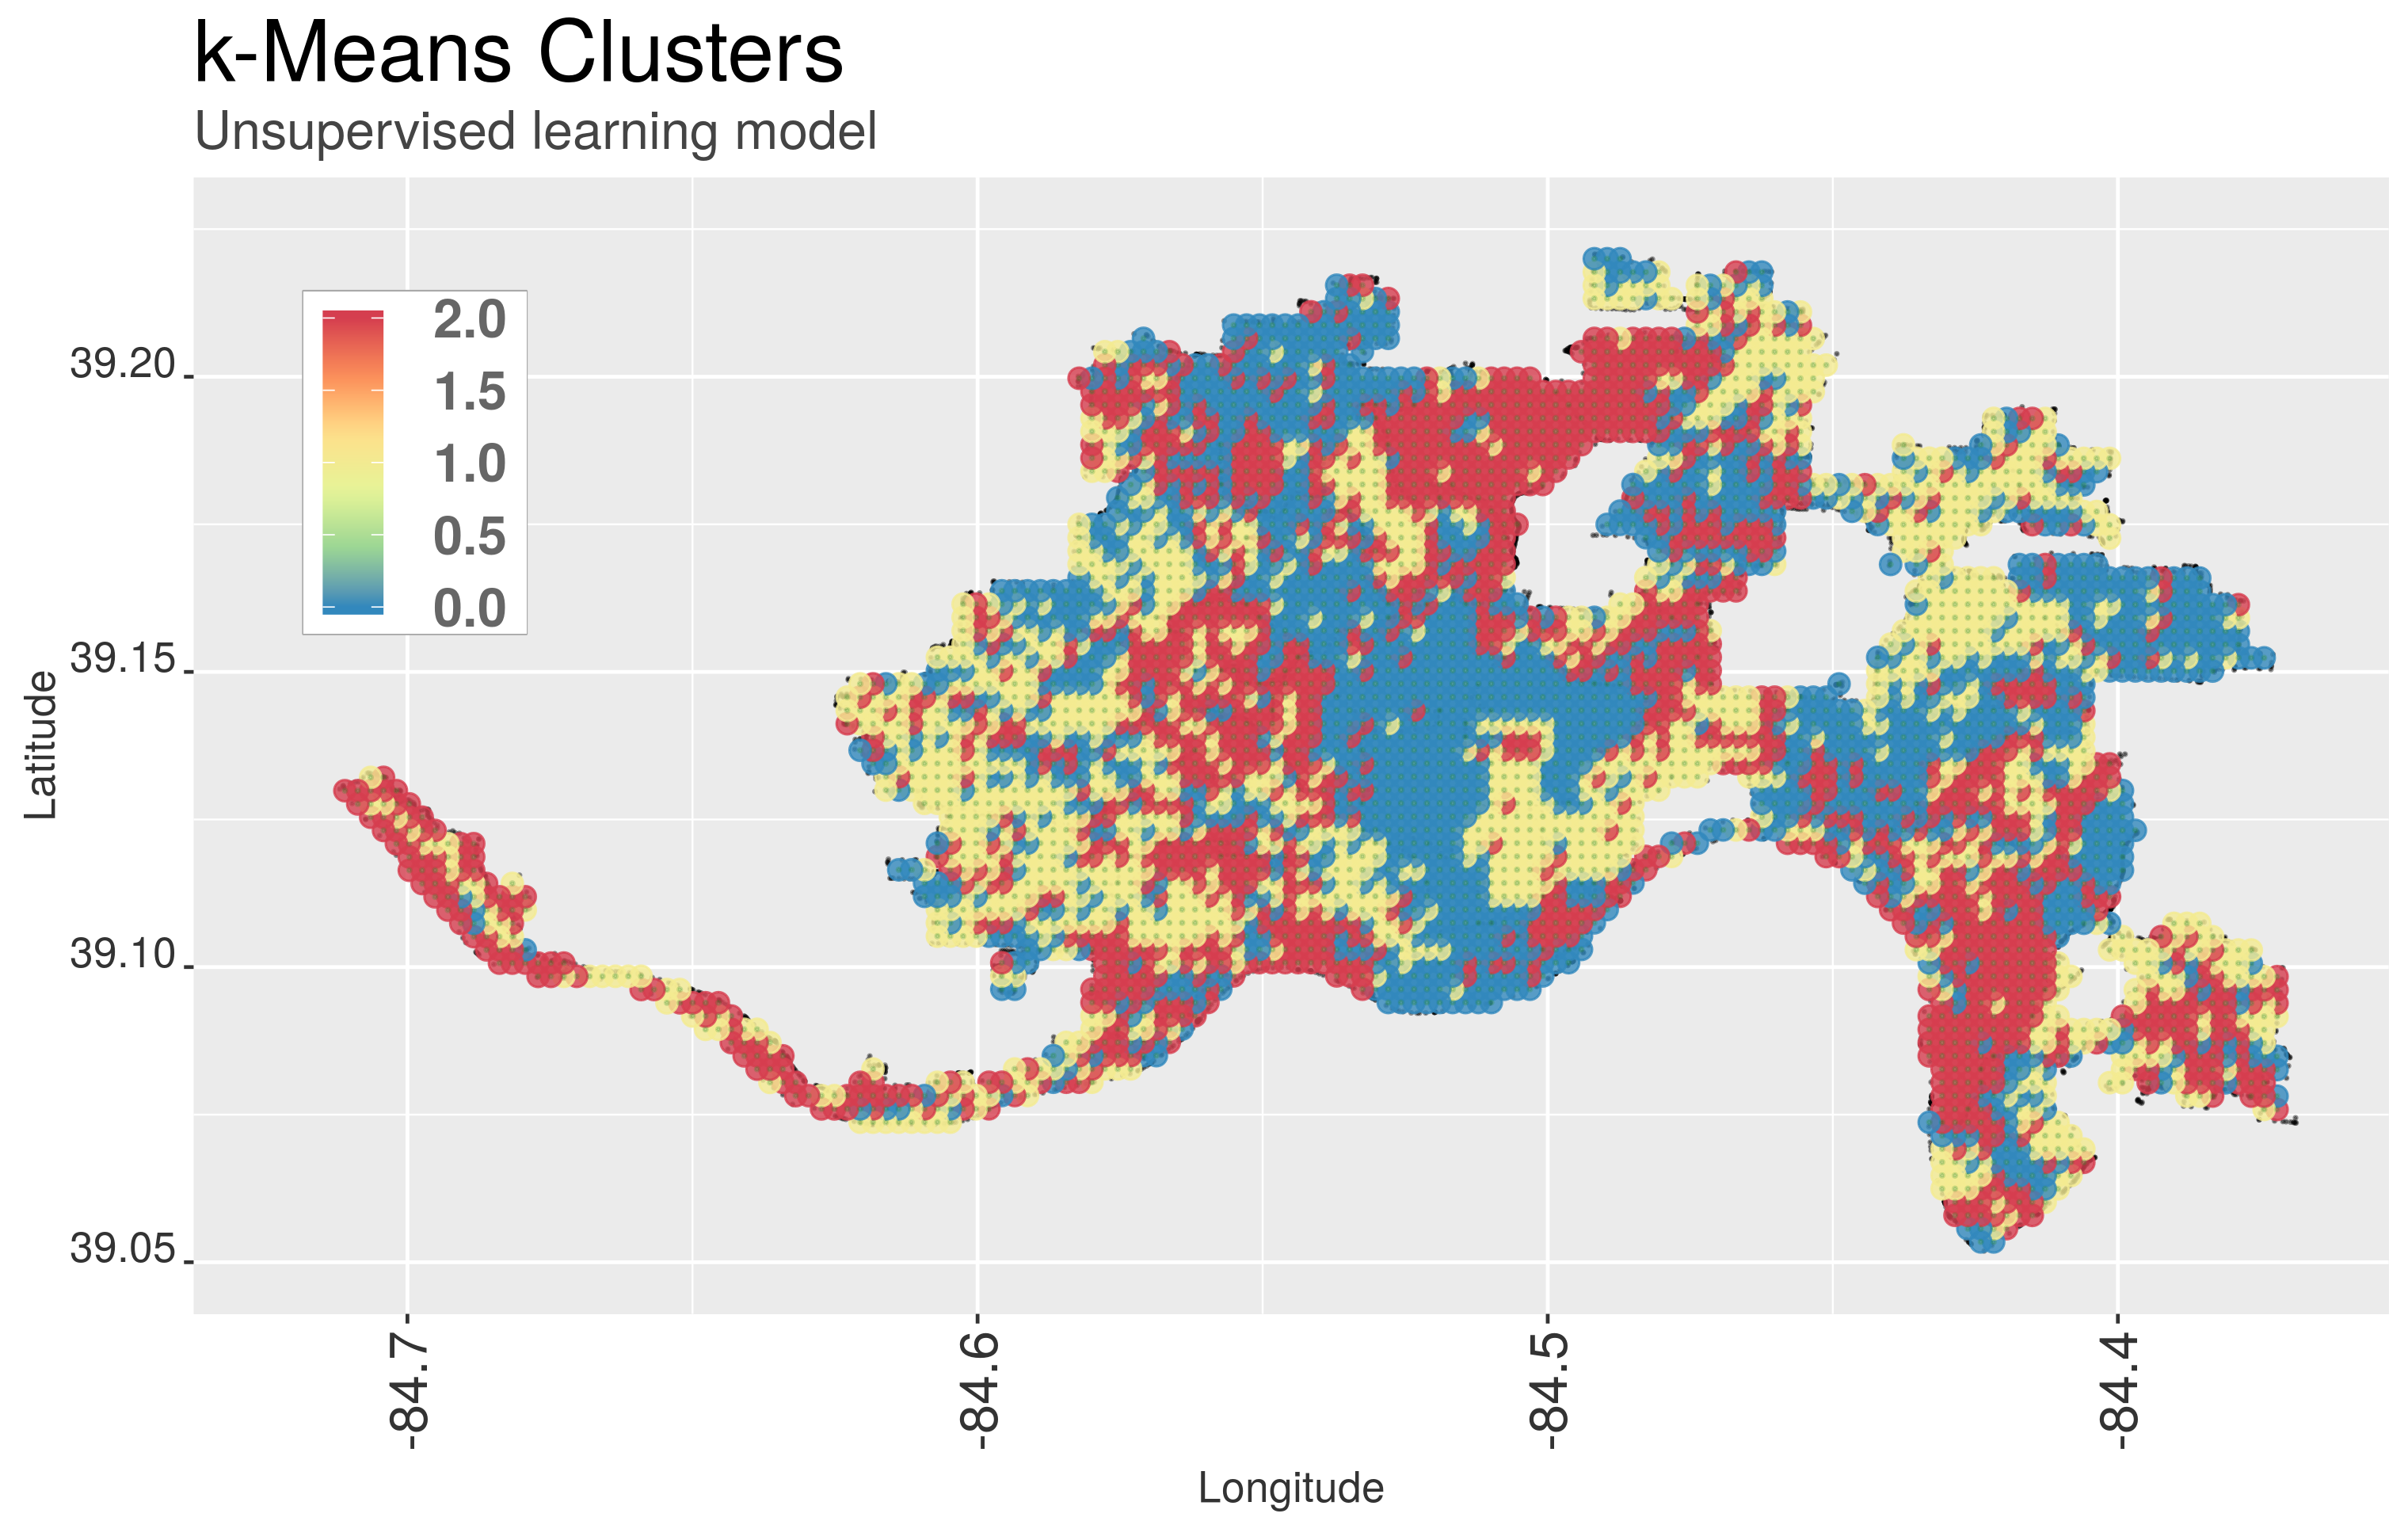
\includegraphics[width=\textwidth, height=\textheight, keepaspectratio]{kmeansongrid.png}
 	\caption{Cluster results on map of Cincinatti}
	\label{figure:kmeansongrid}
\end{figure}
\FloatBarrier

%
\section{Ethics}
%
As a means to evaluate compliance with ethical considerations, we use the model of the ACM Code of Ethics  (the Code). Within the Code, there are four primary sections, e.g., General Ethical Principles, Professional Leadership Principles, etc., with each primary section providing additional subsections for self-assessment compliance to the Code. For each sub-section, we self-scored categorically as either Y, n/a, or D, where Y indicates that the work completed for this project rather obviously complies with the Code, n/a indicates that that section of the Code is less obviously significant for this project, and D indicates that that section of the Code identifies a potential ethical dilemma that is worthy of additional discussion to demonstrate compliance or at least point out the potential ethical challenge identified from this self-assessment.
The most significant elements that we self-assess as D are : \S 1.2 - Avoid harm; \S 1.4 - Be fair and take action not to discriminate; and \S 3.7 - Recognize and take special care of systems that become integrated into the infrastructure of society.

From these three elements, we consider that the significant question to evaluate is: how may these research findings be interpreted and used ?

The result of this project provides a recommended prioritization for the allocation of municipal resources for the purpose of improving a pedestrian safety problem. Allocation of  public resources is often as much a political challenge as it is a scientific challenge. There is no global objective function that assigns absolute social value to any decision of resource allocation. That is, in fact, the work and challenge of public officials. Within the general framework of public decision making it is recognized that facts, reports, and recommendations which are or were essentially the result of objective research are frequently interpreted in a way that suits the interpreter for their own agenda – in some cases for personal gain – financially or politically. We have to admit for this case, then, that this evaluation is potentially subject to a personally motivated interpretation. The debate about using scientific research to guide public policy is long and continuing. With that recognition, the task falls to us to identify what steps are taken to reduce the risk of unintended uses of this report.

First, the report as written has limited scope for direct application to policy. The recommendations included are applicable to the specific time period and data evaluation associated to the City of Cincinnati. The methods presented here can be widely applied (and in fact, that is the goal of this research), but in current form it would be difficult to justify using these results for direct resource allocation in any other municipality. The model developed here used very specific local experiences – accidents, reported near accidents, local conditions survey, property valuations, social media, and all other elements that contributed to this model are local and specific to the City of Cincinnati and to the current time period. As such, the specific recommendations are not generalizable. The method is generalizable; the specific results may provide indications of what local elements in other municipalities may prove indicative or at least useful for a similar exercise, but in any rational discourse, it would be difficult to extend the specific recommendations from this study to municipalities beyond the extent of this study.

Secondly, this report is submitted to representatives of the Cincinnati City Council and the Department of Safety . By distributing the results to more than one department and to a reasonably broad audience reduces risk of information being used for narrowly scoped  or interests which are not generally aligned with good public discussion, debate, and utilization. Further, the data and methods deployed here were developed based on early and continuing input from representatives of these multiple departments within the City. Thus, early and often participation of multiple stakeholders provided the opportunity to have balanced input to the research, thus improving likelihood of balanced output and utilization. And, by respecting and incorporating the input from multiple perspectives from within the City provides higher likelihood of acceptance (and perhaps adoption) of the resulting recommendations.

Thirdly, within the City of Cincinnati, there are currently several on-going initiatives dedicated to improving pedestrian safety. The other initiatives are, in some cases, significantly funded, and are the work product of several departments within the City, predominantly the Department of Safety, that are the prime stakeholders in promoting public safety in the City. These other initiatives are an order of magnitude more significant, both from resource commitment, and for intended impact, than is this study. It is not our aim to minimize the potential impact of the recommendations from this study, but we are cognizant of the relative significance of this study within the larger context of the on-going programs within the City. In any decision making forum for the City, we consider the likelihood of these results having the capability to be used for unintended or inappropriate outcomes to be sufficiently unlikely.

The ethical considerations associated to this project are adequately assessed in the spirit of the ACM Code. The identified risks are appropriately mitigated.
%
\section{Conclusions (and Future Work)}
%

This study demonstrates a methodology to identify areas within the city of Cincinnati, Ohio with the largest potential for safety improvement, based on many open-source datasets made public by the city. Over twenty 250 meter by 250 meter plots of land within the city have been identified for further investigation to determine why the cost of incident within that area are abnormally high as compared to our models. These locations include several areas in the Westwood neighborhood, Clifton, Avondale, Walnut Hills, Bond Hill, and more. Our unsupervised learning techniques… Placeholder sentences about how our unsupervised learning techniques have outlined areas which have potential for safety improvement. These areas demonstrate these qualities which are related to pedestrian safety in the city of Cincinnati, Ohio.

For our unsupervised learning we look at the top pedestrian safety issues in each cluster. Vehicles running red lights or stop signs is a concern for the blue cluster neighborhoods, including: Westwood, Mt. Washington and East End. Heavy traffic is a prominent issue in the green cluster and affects Over-The-Rhine, Mt. Auburn and Central Business District neighborhoods. There is a need for increased number of sidewalks in Clifton, Madisonville, Walnut Hills and Mt. Washington. Over-the-Rhine, Downtown and Clifton need more bike friendly zones.

Future work to further this project could involve the use of other regression modelling techniques to improve accuracy, such as tobit models. Other improvements which could be made include Stuff goes here from Patrick and Preeti about ways to improve your techniques and models.

Aside from improving the models through the use of different techniques, the study itself can be improved by ingesting more data. This study is carried out using publicly available data, if private data exists which can improve the study, it can easily be adapted for use due to only requiring a street address or latitude longitude coordinates which would allow the data to be integrated into the grid-cell aggregation function. Examples of data which may be useful but are not publicly available would be the race, gender and age of the perpetrator and pedestrian victim, data which the city of Cincinnati may have, though the ethical implications of using this data must be weighed.


% ---- Bibliography ----
%
\bibliographystyle{splncs}
\bibliography{pedestrianreferences}

\end{document}